%%%-----------------------%%%
%%%--------PREAMBLE-------%%%
%%%-----------------------%%%

\documentclass[11pt, a4paper]{article}

% Define input coding to UTF8
\usepackage[utf8]{inputenc}

% Package to have abstract environment with correct format (i.e., centered, larger left/right margin, etc.)
\usepackage{abstract}

% Define 1.5pt line spacing
\usepackage{setspace}
\onehalfspacing

% Define the page margins
\usepackage[a4paper, total={6in,9in}]{geometry}

% Package for english language correction and hyphenation
\usepackage[english]{babel}

% Package for "correct" quotation marks
\usepackage{csquotes}

% Package for mathematics
\usepackage{amsmath}
\usepackage{amssymb}

% Define capitalized versions for table alignment -- this allows line breaks yet still positions centered/left/right
\usepackage{tabularx}
\newcolumntype{L}[1]{>{\raggedright\arraybackslash}p{#1}} % linksbündig mit Breitenangabe
\newcolumntype{C}[1]{>{\centering\arraybackslash}p{#1}} % zentriert mit Breitenangabe
\newcolumntype{R}[1]{>{\raggedleft\arraybackslash}p{#1}} % rechtsbündig mit Breitenangabe

% packages for rotating tables
\usepackage{adjustbox}
\usepackage{ctable}
\usepackage{rotating}
\usepackage{pbox}

% Define a colorbox for highlighting terms in math mode
\newcommand{\highlight}[1]{
  \colorbox{light_gray}{$\displaystyle#1$}}

% Package for mathematical macros
\usepackage{mathtools}

% Define the expected value and conditional expectation operators
\newcommand{\expect}{\operatorname{E}\expectarg}
\DeclarePairedDelimiterX{\expectarg}[1]{[}{]}{%
  \ifnum\currentgrouptype=16 \else\begingroup\fi
  \activatebar#1
  \ifnum\currentgrouptype=16 \else\endgroup\fi
}

\newcommand{\innermid}{\nonscript\;\delimsize\vert\nonscript\;}
\newcommand{\activatebar}{%
  \begingroup\lccode`\~=`\|
  \lowercase{\endgroup\let~}\innermid 
  \mathcode`|=\string"8000
}

% define numbering command for (last / specific) line of math arrays
\newcommand\numberthis{\addtocounter{equation}{1}\tag{\theequation}}

% Package to optimize the positioning / float of figures and tables
\usepackage{float}

% Package to have the possibility of modifying the appearance of numbered lists
\usepackage{enumerate}

% Package to define the style of footnotes - with option bottom we place them at the bottom of each page
\usepackage[bottom, hang]{footmisc}

%\restylefloat{table, figure}

% Package for graphs, especially for subfigures 
\usepackage{graphicx}
\usepackage{subfig}

% Package to insert "random" text a la "lorem ipsum"
%%\usepackage{blindtext}

% Package to "shadow" cols/rows of tables and create colored boxes
\usepackage{xcolor}

\newcommand{\cbox}[2][gray]{%
  \colorbox{#1}{\parbox{\dimexpr\linewidth-2\fboxsep}{\strut #2\strut}}%
}
\definecolor{light_gray}{gray}{0.85}

\setlength{\parindent}{0cm}
\setlength{\parskip}{3mm plus1mm minus1mm}

% Caption Package: define the caption of tables to be a bit further down and not "stick" to the table's last row
%%\usepackage{caption} 
%%\captionsetup[table, longtable]{skip = 6pt}

% long tables across multiple pages
\usepackage{longtable}

% format for captions: boldfaced, left-aligned
\captionsetup{labelfont = {bf}, justification = raggedright, singlelinecheck = false, format = hang}
\newcommand{\source}[1]{\caption*{\textbf{Source:} {#1}} }

% Define the paths were graphs and images will be loaded
\graphicspath{{./Images/}{./Results_Images/}{./Results_Tables/}}

% Define the header line
\usepackage{fancyhdr}
\pagestyle{fancy}
\fancyhf{}
%\cfoot{\thepage}
%\chead{{\small \textit{Using Text Sentiment of Company Filings to Forecast Volatility}}}
\chead{\thepage}
%\lhead{Forecasting Realized Equity Volatility From Text Sentiment Revealed by Company Filings}

% Define chapter-wise numbering of figures & tables
\usepackage{chngcntr}
%%\counterwithin{figure}{section}
%%\counterwithin{table}{section}
\counterwithin{equation}{section}

% Package for appendices
\usepackage[toc, page]{appendix}

\usepackage{pdflscape}


% BibLaTex: load package
\usepackage[style=authoryear, date=year, backend=biber, maxbibnames=10, backref=true, backrefstyle=two, doi=false, isbn=false, url=false, maxcitenames=2, dashed=false]{biblatex}
% Note that block = par prints each element (i.e., author name, paper name, journal name, etc.) of the bib entries in a separate line

% Let Biblatex ignore the abstract part of the entries
\DeclareSourcemap{
  \maps[datatype=bibtex]{
    \map{
      \step[fieldset=abstract, null]
    }
  }
}

% put some space between the entries in the bibliography 
\setlength\bibitemsep{0.5\baselineskip}

% Remove quotation marks around titles in the bibliogaphy and remove the italic font 
\DeclareFieldFormat[article, book, inbook, incollection, inproceedings, misc, thesis, unpublished]{title}{#1}

% Remove the "in" before the Journal Name
\renewbibmacro{in:}{}

% Package for hyperlinks and URLs
%\usepackage[colorlinks=true, allcolors=magenta]{hyperref} % for colored links
\usepackage{hyperref} % for uncolored = black links

% Set a high penalty for URLs outside the page margins so as to force a line break in the bibliography
\setcounter{biburllcpenalty}{7000}
\setcounter{biburlucpenalty}{8000}

% Avoid hyphenation in general
\tolerance=1
\emergencystretch=\maxdimen
\hyphenpenalty=7000
\hbadness=7000

% Place all tables and figures at the end of the paper
%%\usepackage[nolists, tabhead, fighead, tablesfirst, heads]{endfloat}
%%\DeclareDelayedFloatFlavor{sidewaystable}{table}

% Auto-generate a list of abbreviations
\usepackage[norefpage]{nomencl}
% Rename the title of the nomenclature to "list of abbrevations"
%%\renewcommand{\nomname}{List of Abbreviations}
% print the abbreviations in bold
%%\def\nomlabel#1{\textbf{#1}\hfil}

% Add .bib database containing all my literature
\addbibresource{./bibliography_database_raw.bib}

\begin{document}
% \newpage
\thispagestyle{empty}
\null
\newpage
\thispagestyle{empty}
\null
\newpage
\thispagestyle{empty}
\vspace*{4cm}
\begin{center}
\textit{{\Large To Mila.}}
\end{center}
\newpage
\thispagestyle{empty}
\null
\clearpage

%%%---------------------------%%%
%%%-------INTRO PART-------       %%%
%%%---------------------------%%%

% format page numbering (intro part with Roman letters, rest of thesis with Arabic letters)
\newpage
%\addchaptertocentry{Abstract} % Add the declaration to the table of contents
\thispagestyle{empty}
\begin{abstract}
In recent times, large scale textual analysis was started to be deployed in finance and accounting analysis. Among others, an established use case happens to be the application of natural language processing for volatility forecasting. In this thesis, I extend existing dictionary-based methodologies in the field of textual sentiment analysis by introducing a term-weighting scheme which is based on the impact of words on past volatility. Using a sample of 46,384 corporate 10-K filings, the learned term weights are aggregated to \enquote{sentiment scores} for out-of-sample 10-K reports. It is found that --  while negative and positive tone embedded in the 10-K do help in explaining post-filing volatility of equity returns -- other textual aspects such as assertiveness/uncertainty in the management's writing style, focus on financial topics, or document readability appear to have insignificant importance for volatility forecasting purposes or carry influential power only in certain years of the test period (2013 - 2017). This notion is confirmed in robustness checks which incorporate variance forecasts from powerful conventional time-series models: after including potent volatility forecasts from the GARCH model family, with the exception of positive and negative sentiment the textual contents embedded in 10-K filings fall short in providing value added for prediction of realized stock return volatility. 
\end{abstract}
\clearpage
\pagenumbering{Roman}
\setcounter{page}{1}
\tableofcontents
\clearpage
%%\listoffigures
%%\clearpage
%%\listoftables
%%\clearpage
%%\makenomenclature
%%\printnomenclature[1.4in]
%%\clearpage
\pagenumbering{arabic}
\setcounter{page}{1}

%%%-----------------------%%%
%%%-------PART TEXT-------%%%
%%%-----------------------%%%

\section{Introduction}
\label{sec: introduction}
Consider the following situation: investor I is offered a choice between two alternatives. In the first scenario, a dice will be rolled and - depending on the number of eyes displayed - a certain amount will be paid to the investor. In case only one pip appears, she receives 100 USD, if two pips appear she will get 200 USD, and so on. Assuming the dice is fair, her expected pay-off from this game will be 350 USD. If the second alternative would be a guaranteed payment of 350 USD, would the investor be willing to take the gamble and roll the dice?

\nomenclature{USD}{US-Dollar}

Most (behavioural) finance research would answer this question with \enquote{no}, with the main argument being similar to: the \textit{rational} investor does not only care about the average pay-off she will receive (which would be the same in both alternative choices of the game), she is also interested in the riskiness as to which this pay-off will occur. Assuming that the average investor will perceive the expected deviation from the mean payment as \enquote{riskiness} (or as it shall be called henceforth: \enquote{volatility}), the second option is clearly preferred; the monetary outcome is secured and is not connected to any uncertainty about the payment of the game whatsoever\footnote{In this game, the first alternative (gamble) exhibits a standard deviation of around 171 USD, while the second alternative (safe payment) has a standard deviation of zero.}. In other words, as \textcite[77]{Markowitz1952} pointed out in his pioneering paper about portfolio theory: \enquote{the investor does (or should) consider expected return a desirable thing and variance of return an undesirable thing.}

Being a variable clearly of interest to investors, the task of forecasting the volatility of financial time series experienced a true \enquote{boom} in the past few decades, in both theoretical as well as empirical research, especially after the publication of two seminal papers by \textcite{Engle1982} and \textcite{Bollerslev1986}, who introduced the (G)ARCH models and were the first ones to model conditional variance series as time series. And also practitioners acknowledge the importance of return variance in real-world financial applications, the most famous probably being derivatives pricing, portfolio selection, and risk management. The latter also increased awareness of regulators with regards to monitoring asset volatility.

Moreover, volatility has become to be considered an \enquote{asset} per se, in the sense that one can speculate on how it will develop in the future. The most famous means to invest in volatility as an asset is using index-tracking instruments which mimick the Chicago Board Options Exchange SPX Volatility Index (usually referred to as VIX). The VIX provides estimates about general market volatility by combining option-implied volatilities at different strikes for single stocks and aggregating them in a weighted-average method. A very recent real-world example demonstrates the importance in an accurate prediction of volatility for investment purposes: in early February 2018, the VIX increased by more than an unprecedented 100 per cent in a single day. Some exchange-traded products, such as the \enquote{Inverse VIX Short-Term exchange-traded note}, issued by Swiss bank Credit Suisse and accordingly named XIV, who bet on the “calmness” of markets, lost a substantial amount of value due to the spike in market volatility. The XIV, for instance, closed almost 80 percent down, leaving the issuer of the securities to experience a siginficant 8.5 percent drop in its share price the subsequent day \parencite{CNBC2018}.

\nomenclature{VIX}{Chicago Board Options Exchange SPX Volatility Index}
\nomenclature{XIV}{Inverse VIX Short-Term Exchange-Traded Note}

Such examples raise the question on what the drivers of an financial asset's volatility are. Focussing on public equity markets, many factors have been used in many models in the attempt to explain volatility. The most \enquote{powerful} proved to be past realizations of volatility; a fact that well describes the empirically observed auto-regressive nature of return variance. It is indeed a \enquote{stylized fact} that volatility tends to occur in so-called \emph{clusters}. This circumstance also strongly connects volatility modelling with time series analysis and forecasting, with the main workhorse being the usage of lagged observations of variance in order to explain it \enquote{today} (and in the future, as well). 
Besides past return series, other authors (such as \textcite{Paye_VolaMacro_2012}) have attempted to add further financial and macroeconomic factors in their predictions (e.g., GDP fluctuations or inflation as explanatory indicators); however, there is little consensus in the literature about the usefulness of such variables in volatility modelling \parencite[2]{MittnikRobinzonovSpindler_2015}. Another driver of volatility has shown to be the so-called (option-price-) implied volatility for single stocks, or, on an aggregate level, the VIX for market-level volatility (cf. \textcite{MittnikRobinzonovSpindler_2015} and referenced literature therein). 

More recently, some authors have also attempted to include what can be called \enquote{soft} or \enquote{qualitative} information in their (volatility) models; very often such variables are used in addition to quantitative data (such as historical time series in prices, returns, or volumes, financial statement and balance sheet metrics, etc.). The latter are \enquote{hard} inputs in the sense that they are observable and verifiable, while qualitative information by nature is more subjective and imprecise \parencite{LM-meta-2016}. The largest part of such soft information content is available in the form of text. However, as \textcite[146]{Das2014} points out, \enquote{until recently, financial analysis was just based on numbers. Usage of text required human coding of attributes into numerical form before yielding to analysis}. Having available computer machines with larger storage capacity, faster processing power and appropriate software to analyze textual inputs, the applications of text mining and processing in the domain of finance and accounting have increased tremendously since the 1990s \parencite{KumarRavi2016}. Representatively of this rising attention towards textual information, well-known economist Hal Varian, when reviewing the paper of \textcite{AntweilerFrank2004} in his New York Times column in 2004, stated: 
\SetBlockThreshold{1}  
\blockquote[\textcite{Varian-NYT-2004}]{In the 1970's we saw the rise of Wall Street quantitative analysts. Then came program trading. Perhaps computational linguistics and textual data mining will become the new hot technologies in financial economics.}

While the terminology of \enquote{text mining} is often used interchangeably with phrases such as computational linguistics, content analysis, natural or statistical language processing, text analytics, information retrireval, stylometrics, etc. \parencite{LM-meta-2016}, the basic concept for the purposes of this thesis can be defined as follows: 
\SetBlockThreshold{1} 
\blockquote[\textcite{Das2014}]{Text mining is the large-scale, automated processing of plain text language in digital form to extract data that is converted into useful quantitative or qualitative information.}

Referring to a meta-study by \textcite{KumarRavi2016}, the applications of text mining techniques within the field of research in the business and economics domain are broad; specifically, they categorize them very broadly into four buckets: \enquote{FOREX rate prediction, stock market prediction, customer relationship management (CRM) and cyber security} \parencite[128]{KumarRavi2016}. However, text mining in the business domain is no longer a purely academic undergoing; real-world applications, for instance, can include the measurement of customer satisfaction and churn likelihood by mining unstructured reviews of clients, the development of early-warning systems for banks that incorporate sentiment information in estimation of default probabilities \parencite{McKinsey_2013}, or the establishment of an internal communication and monitoring tool for companies so to measure employee mood, motivation, or satisfaction \parencite{RMM_2015}. Moreover, the range of applications is very likely to increase in the future, as \enquote{it's not hard to see how almost any business could eventually reap rewards from the ability to comb through the writings of millions of people to identify coming desires and/or needs in entertainment, food, travel, retail -- pretty much anything, in both the consumer and B2B space} \parencite{TIME_2012}. 

Furthermore, irrespective of the actual application framework, the universe of textual sources which can be tapped is very large; a non-exhaustive list might range from brokerage/analyst reports, minutes of board or committee meetings, \textbf{10-K reports} or other filings and prospectuses with the SEC, corporate announcements, customer reviews and forum posts, news articles, social media and blog posts, e-mails, conference call logs, and many more. 10-K* filings of US-companies with the United States Securities and Exchange Commission (henceforth abbreviated using the common acronym SEC), highlighted in bold face, will be the textual corpus under consideration in this thesis\footnote{\label{fn: 10K-def}I will henceforth use the *-notation to denote all variants of 10-K filings. The filing types occurring in the sample of this thesis encompass the following: 10-K, 10-K-A, 10-K405, 10-K405-A, 10-KSB, 10-KSB-A, 10-KT, 10-KT-A, 10KSB, 10KSB-A, 10KSB40, 10KSB40-A, 10KT405 and 10KT405-A. The filing variants 10-K405, 10-K405-A, 10KSB40, 10KSB40-A, 10KT405 and 10KT405-A reports were only allowed up till 2003 and indicate a check-the-box rule (regarding the so-called Regulation S-K or S-B Item 405). KSB reports were eligible for small businesses up till 2009. The interjectional letter \texttt{T} indicates transition reports, while addendum \texttt{-A} indicates amendments to previously filed reports. For details regarding 10-K types, refer to \url{https://help.edgar-online.com/edgar/formtypes.asp} (accessed on 07/30/2018).}, with the final sample containing a rich collection of 46,483 filings from the time period 1999-2017. However, having at hand such a large amount of textual input might bring up problems and obstacles on its own. In this context, \textcite{McKinsey_2013} point out from a practitioner's point of view:
\blockquote{Enormous quantities of textual information are available \textelp{} and it is notoriously difficult to use. \textelp{} The challenges of mining this information and separating the signal from the noise are substantial. \textelp{} A database with news articles on about 1,000 companies easily exceeds 20 GB, orders of magnitude more than a financial database on these companies. Storing this much data is not difficult, but any kind of statistical analysis becomes an \enquote{overnight job}, even with optimized algorithms and systems. \textelp{} Second, textual data are unstructured. While it is relatively easy to analyze financial data in a statistical way — figures become meaningful at a certain size and in relation to sample averages — texts are a priori meaningless to a computer. There are no standard or statistical procedures for a machine to analyze and interpret texts. \textelp{} Third, texts are often ambiguous. \textelp{} In fact, almost all the semantic difficulties of written language pose immense problems for machines.} 

\nomenclature{SEC}{(United States) Securities and Exchange Commission}

When it comes to the techniques available for analyzing textual contents for financial purposes, a lot of methodologies are available, while the most common stream of activity in this domain can be subsumed under the umbrella of \enquote{sentiment analysis}. \textcite{RMM_2015} defines it as follows:
\SetBlockThreshold{1}   
\blockquote{Sentiment analysis studies the mood, opinions and attitudes expressed in written text. It aims to discover the emotions behind words in order to determine whether a communication suggests a positive, negative or neutral sentiment.}

It is the goal of this thesis to combine volatility forecasting with large-scale textual analysis; more specifically, the textual sentiment embedded in 10-K* filings will be extracted in an innovative fashion (sentiment term weighting on the basis of past volatility impact) and then used as an additional explanatory factor in the attempt to predict realized variance after the filing of annual reports. This work thereby contributes to existing literature in two dimensions: research connected to the field of volatility prediction and forecasting as well as textual analysis in finance and accounting. With respect to the first stream of literature, a cross-sectional analysis of 46,483 corporate 10-K filings brings to light that positive and negative sentiment embedded in the reports add incremental value in predicting post-filing realized volatility above a simple past predictor (pre-filing realized volatility) as well as conventional time-series models from the GARCH family. Conversely, more granulated linguistic aspects such as assertiveness, uncertainty, litigiousness, readability, or usage of financial keywords, provide little value added in explaining post-filing realized volatility. The second contribution of this thesis concerns language analysis in the empirical finance domain. In this aspect, a new term-weighting method was introduced: instead of using raw term frequencies or established corpus-related weighting schemes, I applied a market-based methodology, smoothing term counts based on their contribution in explaining volatility after past 10-K filings. Most findings revealed in this work are robust across multiple dimensions, such as choice of training/test sample split, alternative volatility proxies, or selection of term-weighting scheme. One special side-note that was discovered in robustness checks further sets this work in contrast to research results related to equity returns: as was revealed in an extensive analysis, volatility models from the GARCH-family seem to do an accurate job in forecasting, while such precision is not present in models for return series. Thus, textual analysis on return series is leaving \enquote{more room for incremental improvement} coming from qualitative and potentially noisy input features such as text tonality and sentiment.

The remainder of this thesis is structured as follows: section \ref{sec: lit_rev} provides an overview about existing literature and theoretical foundations of volatility forecasting and textual analysis in the finance and accounting domain. Section \ref{sec: sentiment_calcs} provides an overview of how 10-K* filings can be mined in a vector-space framework and in this context also presents the first block of my research framework, the methodology of volatility-impact-based term weighting. Section \ref{sec: volamodel} introduces the second pillar of the research design, i.e., presents the hypotheses which connect the document sentiment scores (and other control variables) with post-filing volatility and describes the econometric model used. Section \ref{sec: data_sample} gives insights about the data collection and cleaning procedures as well as statistical descriptions about the final sample. Section \ref{sec: results} provides the uni- and multivariate estimations and a discussion of the results. Section \ref{sec: robustness} offers some thoughts and examinations regarding result robustness. Section \ref{sec: conclusion} draws final conclusions and offers impulses for future research, especially with regards to alternative research design specifications.
\clearpage
%\label{sec: introduction}
\section{Literature Review and Theoretical Background}
\label{sec: lit_rev}

In this section I will provide an overview about influential literature in the field of textual analysis in finance and accounting, with a particular focus on contributions focussing on sentiment analysis. Moreover, I will elaborate on publications related to the readability of financial documents. Finally, a short summary about literature that uses corporate filings for text analysis purposes is provided. 

% ----------------------------------------------------------- %

\subsection{Text Mining and Natural Language Processing in Finance and Accounting}
\label{ssec: lit_rev_TM_NLP}

As \textcite{YukselturkTucker2015} evidence, research based on content analysis in the areas of accounting and finance has gained significant importance recently, with growing literature available in the fields of corporate disclosure and financial reporting as well as analyst reports; in the same context they also report a \enquote{growing body of research on the impact of tone or sentiment on asset prices and returns} \parencite[871]{YukselturkTucker2015}. 
Excellent meta-studies on the use of textual analysis within finance and accounting are given in \textcite{KearneyLiu2014}\footnote{Especially their Table 1 and Table 3 provide a good overview of influential contributions, grouped by the source of textual inputs used, and the main findings, respectively \parencite[3, 12]{KearneyLiu2014}.}, \textcite{GuoShiTu2017} as well as \textcite{LM-meta-2016}. As the latter point out, the idea of mining textual contents to search for patterns and information has a long tradition and reaches far back into history, ranging from biblical keyword analysis to the dissection of the rhetorical content in political speeches. In more recent times, both large increases in computing power as well as availability of textual material have also encouraged researchers from the finance and accounting disciplines to apply textual analysis in these domains. \textcite[1188]{LM-meta-2016}, with regard to this trend,  trenchantly point out that \enquote{the online availability of news articles, earnings conference calls, Securities and Exchange Commission (SEC) filings, and text from social media provide ample fodder for applying the technology.}  

A generic research design of finance and accounting studies which encompass textual analysis is schematically depicted in Figure \ref{fig: process_schema}: starting with the textual \enquote{underlying}, one usually seeks to extract some output from a collection of documents (often referred to as \textit{corpus}). The desired outputs are various (such as sentiment scores, readability measures, similarity metrics, topic categories, document rankings, and many more); likewise, the methods to extract such variables from text are manifold and can include counting the appearance of certain keywords or chain of words (so called \textit{n-grams}), semantic decompositions, the classification of sentences, paragraphs, or documents, or more sophisticated machine learning algorithms such as support vector methods or neural networks. These text-related outputs are then usually connected with quantitative information, whereas tools range from established statistical and econometric procedures (mostly linear or logistic regression) to more advanced fusion methods that involve algorithms from machine learning.

In general, however, natural language processing in the financial domain brings up several obstacles and difficulties for the researcher. A fundamental question is related to an essential trade-off between signal and noise when choosing the research design; in other words, although analyses sometimes use simplifying assumptions\footnote{Most often this assumption reflects the idea that documents can be represented as so-called bags of words which allow the researcher to conduct an analysis on token-level, while at the same time this approach assumes that the ordering of words within a documents is irrelevant. I will further elaborate on this assumption in section \ref{ssec: senti_counts}, when I introduce the vector space model that will be the starting point for the analysis in this thesis.}, the attempt to better capture meaning and context also from a syntactic and semantic point of view can in some cases do more harm than good, because one simply adds more noise to the model that shall not be mistaken for signal \parencite{LM-meta-2016}. 

Further issues, which affect a lot of studies, are data availability, retrieval issues such as downloadability, document structure, and the subsequent parsing process. For some corpora, no collections or databases are available and require download by hand. Moreover, the downloaded files are often not available in the required format or are not machine-readable\footnote{In most cases, the property of being machine-readable is a minimum requirement for any corpus, so this is a rather theoretical side-note.}, or require at least a minimum amount of parsing. This imposes large practical problems, as \enquote{document parsing relies on consistency in the structure of the text and any related markup language} \parencite[1192]{LM-meta-2016}. This requirement is not always given in real-life applications, where data is often unstructured or inconsistent (over time)\footnote{One such issue will be further explained in the description of the corpus of 10-K* filings used in this thesis (see section \ref{sec: data_sample} about data collection and, specifically, footnote \ref{fn: parsing_LM})}. Other problems connected to the parsing procedure arise at the stage of tokenization or sentence-/paragraph-level segmentation. In this context, \textcite[1215]{LM-meta-2016} provide a good introductory overview of challenges and tripwires when applying natural language processing in the financial domain. In particular, the authors highlight issues which arise from what might sound like an obvious statement, namely that\enquote{all textual methods are based on first identifying words}. However, the undergoing of identifying \textit{words} is more subtle than it appears at first sight. One needs to clarify what happens, for instance, with compound words that are connected via hyphens (e.g., \textsf{well-known} or \textsf{up-to-date}), proper nouns (e.g., the \textsf{Fama} and \textsf{French} from the Fama-French-Model), and abbreviations (e.g., \textsf{FC} for football club or \textsf{Mr.} for Mister). Moreover, the example chosen for proper nouns reveals yet another problem: how can one deal with polysemy, i.e., the fact that the surname \textsf{French} (of famous economist Kenneth French) looks fully equivalent to the description of nationality (\enquote{to be of \textsf{French} origin/nationality}), yet the two words have very different meanings? This would require the researcher or the machine to learn from context, which in turn calls for usage of constructs that go above the granularity of a word-based analysis. For instance, this could be learned using n-grams (recognizing that the name \textsf{French} will likely tend to co-occur with words like \textsf{Mr.}, \textsf{Fama}, \textsf{Model}, etc.; whereas the nation-based version will rather co-occur with \textsf{British}, \textsf{German}, and so on). Furthermore, conjugations and declinations can impose problems: words like \textsf{calculate, calculates, calculated, calculating}, etc. all refer to the same word stem, yet are treated differently just because of their suffix. As will described in section \ref{ssec: senti_counts}, lemmatization and stemming deal with that exact problem -- in most cases by chopping off the endings and summing up those four instances as one single token (\textsf{calculat}). 

Similarly, also an apparently trivial task like splitting a document into sentences can prove to be tricky in practice. Generally, the parsing algorithm needs to be instructed on how to treat common sentence delimiters such as periods (\textsf{.}), colons (\textsf{;}), question marks (\textsf{?}), or exclamation marks (\textsf{!}). As \textcite[1216]{LM-meta-2016} evidence, the usage of \enquote{extensive lists, technical terminology, and other formatting complexities, makes sentence disambiguation especially challenging in accounting disclosures}. An illustrative example of this challenge would be the treatment of section headers such as \textsf{2.1. Financial Statements} or decimal separators as in \textsf{199.99 USD}. An inaccurate parser will -- based on the presence of the period sign -- mistakenly split the document at these points; and \enquote{the parsing errors in this case can be extraordinary}, implying that \enquote{Generic sentence parsing algorithms do not work well on financial documents} \parencite[1216, 1217]{LM-meta-2016}. This imprecision has crucial impact on the variable construction, implying the latter are therefore inherently measured with noise. For instance, most document readability measures are constructed using the number of sentences in a document; and thus critically depend on how accurately sentences can be identified.

\subsubsection{Readability}
\label{sssec: lit_rev_mining_readability}
Pioneering contributions in the stream of literature connected to readability of finance- and accounting corpora are \textcite{Li2008}, who evidenced that firms with lower current earnings (or earnings decreases) on average tend to produce less readable as well as longer 10-K filings\footnote{The argument provided suggests that management has an inclination to produce longer and more complex 10-K filings so as to diffuse or dilute bad news to investors. \textcite[221]{Li2008} labels this phenomenon \enquote{management obfuscation hypothesis}.}, and \textcite{DeFranco2015}. While the former \enquote{suggests a clear correlation between the linguistic features of annual reports and firm performance} \parencite[222]{Li2008}, \textcite{DeFranco2015} investigate the readability of security analysts' research reports. They find report readability to positively influence stock trading volume\footnote{A potential explanation for this reads as follows: if a report, ceteris paribus, classifies as \enquote{more readable}, the information conveyed in the document will be perceived as more precise information and thus trigger stronger trading signals for investors \parencite{DeFranco2015}.}, with the latter being a commonly used predictor for stock return volatility and thus relating to this thesis indirectly.

In a similar setting, \textcite{HsiehHuiZhang2016} relate stock price reactions to the degree of readability upon publication of analyst reports. They find that the cumulative abnormal return (CAR) in a $[-1,1]$-day window around the report issuance date increases by 58 basis points if the readability of the report increases by one standard deviation. A particularly important side note for this thesis is the statistical significance that \textcite{HsiehHuiZhang2016} as well as \textcite{DeFranco2015} find for one of their control variables, namely the narrative tone that analysts use -- thus indicating that not only readability but also textual sentiment matters for the market in determining price and volume for equity instruments\footnote{\textcite{DeFranco2015} additionally include an interaction term between readability and tone, which they find to be positive and significant. This suggests that these two variables reinforce each other.}.

% COULD INCLUDE THIS INTERACTION VARIABLE AS WELL .....

\nomenclature{CAR}{Cumulative Abnormal Return}

In the area of volatility prediction based on readability of financial documents, the most relevant paper for this thesis is \textcite{Loughran2014}. They evidence that volatility significantly decreases with the degree of readability of 10-K reports. Suggesting another, more indirect, channel of cause and effect in this context, \textcite{LehavyLiMerkley2011} have shown that less readable 10-K filings tend to be connected with increased analyst coverage\footnote{The authors provide a potential explanation for that phenomenon: a 10-K that is relatively difficult to read has too high processing costs for a single analyst to cover them. Thus, naturally, in order to meet investor's information demand, more analysts will start to track the stock and exert collective effort.}. Referring to the findings of \textcite{Schutte2007}, who evidence that analyst coverage initiation helps investors to better distinguish \enquote{true} firm-specific information from pure noise signals, it can be inferred that the fact that an analyst tracks the company \textit{per se} has a negative impact on firm-specific volatility. This interpretation undermines the findings of \textcite{Loughran2014}, namely that more readability in 10-K's (be it directly or via increased analyst coverage) reduces the stock price volatility of the companies submitting the filings.

Regarding the \textbf{measurement} of readability, different metrics have evolved in the literature, with the most commonly used being the Gunning-Fog-Index as well as the Flesch-Kincaid-Grade-Level-Formula and the Flesch Reading-Ease Score (FRES)\footnote{All of these measures effectively are a linear combination of two components, namely the average length of sentences as well as proportion of \enquote{complex} words used, while complexity of words is determined by syllabication. A more detailed definition of these metrics is provided in appendix \ref{sec: annex_fogflesch}.}; nevertheless, \textcite[1649]{Loughran2014} argue that these measures, because of their strong focus on sentence length and word complexity, are not suitable in the context of business-related text. Moreover, they do not adequately account for differences in background knowledge between the targeted audiences. In fact, based on the Fog measure, very common words like \textsf{company}, \textsf{management}, or \textsf{financial} would be considered to be \enquote{complex} words -- yet they are still very likely to be understood by the average investor. Furthermore, all of the common readability measures require some form of text parsing and are thus exposed to typical inaccuracies and subjectivities connected to such procedures. In the work of \textcite{Loughran2014}, the \enquote{underlying} textual source were 10-K filings with the SEC. For these documents the authors suggest an alternative that is a much simpler, less error-prone and more reproducible metric, yet is still correlated to \enquote{conventional} measures like the Fog Index and equally able to capture readability: the natural logarithm of gross file size (measured in megabytes) of the 10-K filing\footnote{One should note at this stage that this approach requires the researcher to account for firm complexity (most likely using a proxy like firm size), as longer reports could be simply due to the complexity of the fundamental business \parencite{LM-meta-2016}. }.

\nomenclature{FRES}{Flesch Reading-Ease Score}

\subsubsection{Sentiment Analysis}
\label{sssec: lit_rev_mining_senti}

As \textcite{LM-meta-2016} indicate, the most simple approach to a textual analysis with financial corpora is to search the documents for appearance of certain keywords (or keyword phrases) of interest (for instance, they cite phrases like \textsf{ethic} or \textsf{corporate social responsibility}, whose frequency can be used when one attempts to quantify corporate governance metrics or the probability of lawsuits). A natural extension of this methodology involves to not look for specific phrases only, but rather use a dictionary of words\footnote{Throughout this thesis the words lexicon, dictionary, or (sentiment) word list will be used interchangeably; although from a linguistic and literary point of view they are not equivalent.}, all of which carry similar characteristics. In the large majority of cases these word lists are chosen so as to share common sentiment and thus relate directly to the technique of sentiment analysis. 

The frequency of sentiment words is then often aggregated into a scalar, constructing what is often referred to as \enquote{sentiment index} or \enquote{sentiment score}\footnote{Note that the strong focus on keyword counting in sentiment analysis has lead the discipline to be dominated by vector space models (or, equivalently, term-document-matrices) within the bag-of-words framework (see section \ref{ssec: senti_counts} where these concepts will be expanded in the process of introducing the research design applied in this thesis.}. Apart from the usability as a variable in many research applications, sentiment indices are common also in practice, as the following quote undermines:
\blockquote[\textcite{McKinsey_2013}]{Gauging sentiment with an index makes it possible for machines to analyse the information; it can be converted, aggregated, and compared. And the index can be used with statistical analysis to build prediction models. Obviously, the difficulties come in the details of assigning the sentiment index. At the core of the process is a lexicon that lists words or phrases that represent a certain kind of sentiment and, importantly, reflect the specific context in which the text appears.}

The last part of the definition highlights a critical fact that distinguishes sentiment analysis in finance and accounting from other disciplines: while early studies used \enquote{generic} lexica\footnote{The most prominent choice for word classification among the heap of lexica available was the Harvard General Inquirer (GI) (in particular, the Harvard IV-4 dictionary, see \url{http://www.wjh.harvard.edu/~inquirer/homecat.htm}).} that were developed from (and thus suitable for) texts in psychology and sociology, \textcite{Loughran2011} were the first to recognize that those lists are not applicable to documents in the business domain. In fact, using 10-K filings, the authors find that almost three quarters of allegedly negative words in the Harvard IV-4 list do not appear to be negative in business context\footnote{For instance, such words are \textsf{tax, cost, capital, board, liability, foreign}, and \textsf{vice}, which appear very often in 10-K filings, yet are very likely not negatively connoted \parencite[36]{Loughran2011}.}. Therefore, \textcite{Loughran2011} created finance-specific sentiment word lists in the following categories: negative, positive, uncertainty, constraining, litigious, strong/modest/weak modal. These lists (especially the negative lexicon) have become the \enquote{gold standard} in financial sentiment analysis and are also the backbone of this thesis. Henceforth, I will label these word lists using the acronym LM dictionary (or lexicon/word list). 

\nomenclature{LM (Dictionaries)}{Sentiment Dictionaries developed in \textcite{Loughran2011}}

Turning from this methodological introduction to relevant literature contributions, a good starting point for dictionary-based sentiment extraction is the paper of \textcite{YukselturkTucker2015}. They calculate thematic net sentiment scores for a UK-based sample of analyst research reports by classifying (80 to 180) keywords contained in six theme-buckets\footnote{The six themes are the following: macroeconomic and regulatory environment, industry and market environment, growth, management and strategy, financial performance, financial position.} into positive and negative keywords, while the classification task was performed using both Harvard IV-4 and LM dictionaries. The main finding was that theme-related (net) sentiment affects the two key outputs (recommendations and target prices) of the research analyst. \textcite{HuangZangZheng14} extended this stream of research regarding textual contents of analyst reports. They quantified sentiment of sentences contained in analyst reports using a Naive Bayes machine-learning algorithm. After controlling for a simultaneous change in the quantitative summary metrics (i.e., price target, stock recommendation and EPS forecast), they show that the textual opinion embedded in the respective analyst report helps to explain abnormal stock returns subsequent to the release of the report. Moreover, they evidence that the narrative content of analyst reports also carries \enquote {predictive value for future earnings growth in the subsequent five years} \parencite[2151]{HuangZangZheng14}. 

In the same category of research falls also an important paper of \textcite{Tetlock2007}. He mined a popular column in the \textit{Wall Street Journal} in order to gauge market sentiment; in particular, he constructed a pessimism index using the Harvard GI lexicon, which was shown to be predictive for lower subsequent returns and higher volatility.

Another pioneering paper in this area of research, which due to its nexus to volatility prediction is also relevant for this work, is \textcite{AntweilerFrank2004}. They analyzed more than 1.5 million messages from message boards about 45 companies; using the Naive Bayes approach to classify messages to either buy, hold, or sell category. The single classified messages were then aggregated into a bullishness as well as an agreement index, which proved to be successful in predicting both trading volume and volatility, but unsuccessful in explaining stock returns. Regarding volatility, only the bullishness seems to carry explanatory power while the correlation is positive (i.e., more bullish messages today imply greater volatility tomorrow), while agreement between message posters does not help to predict realized volatility. 

Most importantly, however, this thesis builds upon the work in \textcite{Kogan2009_1}, which was extended in \textcite{TsaiWang2012, TsaiWang2013, TsaiWang2014, TsaiWangChien2016, WangTsaiLiuChang2013} and \textcite{TsaiWang2016}; all of which essentially show that textual sentiment of 10-K's helps to explain stock return volatility in the quarter/year after the filing (either in a ranking or regression framework). These results were yet further refined in \textcite{Rekabsaz2017}, who used a more elaborate word weighting scheme on the LM sentiment lists and also investigated on potential industry-specific patterns. 

\subsubsection{Text Analysis Using 10-K Filings Corpora}
\label{sssec: lit_rev_mining_10K}

As it is evident from the literature review up to this point, corporate filings as a mandatorily disclosed document provide a rich source of potential research questions in the textual analytics field and are very popular within the finance and accounting domain. In this context, \textcite[223]{Das2014} points out\footnote{In that regard, \textcite[3]{KearneyLiu2014} highlight that while corporate disclosures provide \enquote{a natural source of textual sentiment for researchers insofar as they are official releases}, their main disadvantage \enquote{is the low frequency of the data, because firms usually make these disclosures on a quarterly or annual basis.}}: 
\blockquote{Whereas much of financial text analysis uses messages posted to finance boards like Yahoo!, Motley Fool, or to blogs such as Twitter, Facebook, etc., other textual analysis has been applied to company reports and filings. In the former case, analysis is usually of a time series nature, whereas in the latter, text analysis is undertaken across companies in a cross-section.}

Regarding the heap of corporate filings available, \textcite[227]{Das2014} further highlights that most of the literature is focussing on 10-K filings because these are considered to be the most informative document for (potential) investors\footnote{I follow this stream of literature and use a broad corpus of 10-K*s (refer to footnote \ref{fn: 10K-def} for a description of variants of the \enquote{standard} 10-K). Moreover, to avoid permanent repetition I will use the terms 10-K, filing, or (annual) report synonymously, although the SEC highlights that \enquote{10-K typically includes more detailed information than the annual report to shareholders.} (see \url{https://www.sec.gov/fast-answers/answersreada10khtm.html}, visited on 05/27/2018)}. 10-K reports are mandatory disclosure documents that are to be filed annually with the SEC. As it is outlined on their web-page\footnote{See \url{https://www.sec.gov/fast-answers/answersreada10khtm.html}, accessed on 07/31/2018.}, the report's contents contain an important source of information and decision-making material for investors: \enquote{Among other things, the 10-K offers a detailed picture of a company's business, the risks it faces, and the operating and financial results for the fiscal year. Company management also discusses its perspective on the business results and what is driving them.} As \textcite{Pulliza2015} points out and what is of direct importance for all language analytics studies using this corpus, 10-K filings shall be conform with the SEC Plain English Rule, which was established with the target that communication from the management towards the investor community is written in plain and understandable terms without an overload of complexity.

One should note that this part of the literature review reflects only \enquote{related} contributions, i.e., publications with a focus on natural language processing and, more specifically, sentiment analysis. The (much broader) stream of literature that deals with the \enquote{quantitative} outputs of (mandatory) corporate disclosure and the information content as well as the market reactions of such disclosures, is not part of this review. This, for instance, encompasses a large range of publications in the field of accounting policies (accounting standards, international comparisons, etc.) and manipulation methods (with contributions related to (abnormal) accruals mainly) as well as mergers and acquisitions including the subsequent purchase price allocations (with contributions related to intangible assets, goodwill, etc.) that are disclosed in annual filings. In fact, I view the combination of such \enquote{hard} information content with the textual tone as a much desired extension for further research; a fact on which I will further elaborate in the conclusions of this thesis (cf. section \ref{sec: conclusion}). 

One of the first questions to ask when analyzing 10-K filings is whether to text mine the whole document or rather target a specific section in it. The most famous of them, which is often said to be the most informative part and carry the most forward-looking statements, is Item 7 of the 10-K filing, which is referred to as \textit{Management Discussion and Analysis} (MD\&A). For instance, this section is the subject of study in widely cited papers like \textcite{Kogan2009_1, Li2010, Feldman_et_al_2010, TsaiWang2012, WangTsaiLiuChang2013, TsaiWang2013, TsaiWangChien2016, TsaiWang2016}. 

Another common choice is \textit{Item 1A - Risk Factors}, \enquote{which contains information about the most significant risks for the company} \parencite[1712]{Rekabsaz2017}, which is used, among others, in \textcite{HuangLi2011} and \textcite{Rekabsaz2017}. A good overview of all sections within a 10-K filing is provided on the SEC web-page\footnote{See \url{https://www.sec.gov/fast-answers/answersreada10khtm.html}, accessed on 7/31/2018}.  

However, also section-based analysis comes with obstacles: as \textcite{LM-meta-2016} evidence, parsing algorithms struggle with the fact that some 10-K submissions are unstructured (especially before 2002), some sections are mislabelled (e.g., MD\&A is falsely tagged as Item 6 instead of 7), or that companies place content across different parts of the document and cross-reference across the filing using footnotes. Regarding the latter, \textcite{HeidariFelden_Footnotes_2015} presented a promising idea, that might be an interesting extension to 10-K corpus based research: they tried to categorize income tax footnotes within 10-K and 10-Q's into pre-defined buckets and proved that machine-based classifiers can achieve the same task with relatively high accuracy, allowing the researcher to extract content from an \enquote{unstructured} part of the filing without the necessity of reading the footnotes manually. This was extended upon by \textcite{Amel-Zadeh_Faasse_2016} and \textcite{ThinggaardJeppersenMadsen2016}, who compared MD\&A content with footnote disclosure, the latter doing so for the Danish market and therefore belonging to the absolute minority of publications which use non-US based data.

The most influential papers who focus on the 10-K as single, homogeneous document are \textcite{KothariLiShort_2009, LehavyLiMerkley2011, Loughran2011, Loughran2014, LM-meta-2016}, while good introductory overviews about 10-K language processing (and, more generally, textual analysis in finance and accounting) are provided by \textcite{Qiu07, Pulliza2015, LM-meta-2016}. 

\nomenclature{MD\&A}{Management Discussion and Analysis (Section within a 10-K Filing)}

\clearpage
%\label{sec: lit_rev}
\section{Term Weighting and Calculation of Sentiment Scores}
\label{sec: sentiment_calcs}
This section outlines the first part of my research framework, namely the sentiment extraction process from the 10-K* filings. Starting with simple term counts and conventional weighting schemes, in the course of this section, I will also introduce the \enquote{volatility-impact-based} term weighting building on \textcite{Jegadeesh2013}; in this context, the volatility measure applied in this thesis will be explained. Moreover, the section also describes the aggregation of (weighted) sentiment frequencies into sentiment scores.

% ----------------------------------------------------------- %

\subsection{Term Counts, Document-Term-Matrix, and Vector Space Model}
\label{ssec: senti_counts}
\nomenclature{TDM}{Term-Document-Matrix}
\nomenclature{DTM}{Document-Term-Matrix}
\nomenclature{BoW}{Bag of Words}
% Circumvent the problem of Latex to not put % sign in an URL in a footnote by declaring "myurl"
\urldef\myurl\url{https://sraf.nd.edu/textual-analysis/resources/#Master%20Dictionary}

When considering sentiment analysis, a common starting point is the representation of the textual corpus $\mathcal{D}$ in a so-called document-term-matrix, commonly abbreviated by DTM\footnote{One can, alternatively, also transpose the matrix and represent the corpus as a term-document-matrix, TDM.}. As indicated, a corpus, denoted by $\mathcal{D}$, is simply a collection of $N$ different documents which the researcher seeks to analyze, i.e., $\mathcal{D}  = \{d_1, d_2, \dots, d_N \}$. Thus, in a DTM each of the rows of the DTM is representing one document $d_i$, $i = 1, \dots, N$, from corpus $\mathcal{D}$. In the case of this thesis, this corresponds to one 10-K* filing per row. Similarly, each column stands for one word \textit{type} in the available vocabulary\footnote{Althoug henceforth the term \enquote{word} will be used synonymously to the phrase \enquote{word type}, it is at this stage useful to briefly present an important concept in text analysis: the distinction of word \textbf{type} and \textbf{token}. While types represent the number of \textit{distinct} words within a corpus, tokens are the total number of all words \parencite{Jurafsky_Draft_2017}. Very common phrases like \textsf{and}, which appear very often in the corpus, imply that there are many tokens for this word but in fact only one type. This also highlights the usefulness of a matrix representation, in which one can take account for multiple occurrences of a word type by displaying its \textit{count}.}. The vocabulary in turn can be either formed in a \enquote{naive} way, i.e., include all terms that appear in the full corpus at least once (in other words, in at least one document) or, alternatively, contain only pre-selected words from a given lexicon. In this thesis, I will use eight different lexica produced by \textcite{Loughran2011}. The main reasons for this are indicated in the enumerated list in the subsequent section \ref{ssec: DTM_dimensionality}, in which I discuss crucial elements in determining the size of the vocabulary. Henceforth I will indicate the corresponding LM-lexicon to which a word belongs by using sub- and superscript $k$, with $k \in \{N, P, U, L, C, SM, MM, WM\}$, which stand for negative, positive, uncertainty, litigious, constraining, strong modal, modest modal, and weak modal, respectively\footnote{All dictionaries are provided by \textcite{Loughran2011} (\myurl). The constraining as well as weak and modest modal word lists are used in the linguistic analysis only, but are unrelated to the research hypotheses presented in this thesis (see chapter \ref{sec: volamodel}).}. Details on the LM word lists and their composition can be found in Appendix \ref{sec: annex_lm-lists}. The dictionary of category $k$, denoted by $\mathcal{J}_k$, has length $J_k$, i.e., consists of $J_k$ different words labelled $v_{1,k}, v_{2,k}, \dots, v_{J_{k},k}$. Thus, one can write the resulting eight DTM's in the following general notation:
\begin{equation}
DTM_k = 
\bordermatrix{
  & v_{1,k}	& v_{2,k}   & \dots   & v_{J_{k},k} \cr
d_1 & tf_{1,1}^{k} & tf_{1,2}^{k} & \dots & tf_{1,J_{k}}^{k} \cr
d_2 & tf_{2,1}^{k} & tf_{2,2}^{k} & \dots & tf_{2,J_{k}}^{k} \cr
\vdots & \vdots & \vdots & \ddots & \vdots \cr
d_N & tf_{N,1}^{k} & tf_{N,2}^{k} & \dots & tf_{N,J_{k}}^{k} \cr
}
\end{equation}

As said, $DTM_k$ has dimension $N \times J_k$, where the row dimension, $N$, represents the number of documents (i.e., 10-K* filings) in the corpus. The number of columns, $J_k$, denotes the number of sentiment words $v_{j,k}$, $j = 1, 2, \dots, J_{k}$, available in the LM dictionary of category $k$\footnote{One further remark can be made regarding the lexicon size: if one were to create one \enquote{global} DTM with all $J$ (stemmed) word types (coming from all eight available LM dictionaries), the dimensionality would not simply add up: Thus, $J = 1,574 < J_N + J_P + J_U + J_L + J_C + J_{SM} + J_{MM} + J_{WM} = 1,714$. The inequality comes from the fact that the sets $\mathcal{J}_k$ are not disjoint (i.e., several words occur in more than one list). For instance, the uncertainty and litigious sub-lexicon share some common words with the negative word list. Details regarding the LM lexica as well as their overlap are outlined in Appendix \ref{sec: annex_lm-lists}.}. Finally, and most importantly, each coefficient of the DTM, $tf_{i,j}^{k}$, with $i = 1, \dots, N$ and $j = 1, \dots, J_k$, denotes the number of occurrences of word type $j$ from LM-list $k$ in document $i$ (so-called raw \enquote{term frequency} (TF))\footnote{\label{fn: td_incidence_mat}There are also \enquote{simpler} variants of the DTM in which the coefficients do not represent the absolute term frequencies, but rather an indicator variable, i.e., a Boolean equalling one if the term appears (at least once) in the document, and zero else. This is often referred to as term-document \textbf{incidence} matrix \parencite[4]{ManningSchutze_IR_2008}.}. 

\nomenclature{TF}{Term Frequency}

Inspecting the rows of the DTM, one can see that each of the $N$ documents can be represented as an $J_k$-dimensional vector of word counts. Thus, this formulation is often referred to as \enquote{Vector Space Model} and is especially common in information retrieval applications, as it intuitively formalizes the idea that two similar documents will tend to contain comparable sets of words. Hence, their word count vectors should also be similar\footnote{The general task in information retrieval would be the detection of a set of documents, each represented by a $J_k$-dimensional document vector $\mathbf{D}$, that are most similar to a given set of search-/keywords, represented by a $J_k$-dimensional query vector $\mathbf{q}$. The similarity between two vectors in most applications is measured by so-called \textbf{cosine similarity}, i.e., the cosine of the angle that is spanned between the two vectors. Mathematically, one takes use of the notion of dot product and defines: 
\begin{equation*}
\cos(\theta) = \dfrac{\mathbf{D} \cdot \mathbf{q}}{\lVert \mathbf{D} \rVert \cdot \lVert \mathbf{q} \rVert} = \dfrac{\sum_{j=1}^{J_k} D_j q_j}{\sqrt{\sum_{j=1}^{J_k} D_j^2} \sqrt{\sum_{j=1}^{J_k} q_j^2}},
\end{equation*}
where $\lVert \mathbf{z} \rVert$ is called the \textbf{Euclidian norm} (commonly referred to as \enquote{length}) of the vector $\mathbf{z}$ and is used \enquote{normalize} vectors of differing lengths. Generally, $\cos(\theta) = -1$ for vectors pointing in opposite directions, $\cos(\theta) = 0$ for orthogonal vectors, and $\cos(\theta) = 1$ for vectors pointing in the same direction. However, as word counts are always non-negative ($tf_{i,j}^{k} \geq 0$), cosine similarity in text classification problems always lies between zero and unity \parencite[280]{Jurafsky_Draft_2017}.}. However, it is of crucial importance to note an underlying assumption that is implicitly made, if one seeks to represent the corpus in a DTM: if all documents can be displayed as vectors of term counts, the ordering of the words within the document is lost. This is commonly referred to as \textbf{bag-of-words} assumption; specifically, one represents each document as \enquote{an unordered set of words with their position ignored, keeping only their frequency in the document} \parencite[76]{Jurafsky_Draft_2017}. Therefore, the two sentences \textsf{Martin is faster than Tom} and \textsf{Tom is faster than Martin} have two equivalent bag-of-words vector representations, although their meaning is oppositional. 

Besides the implicit bag-of-word assumption, another common feature of vector spaces, also due to the often very high dimensionality of the DTM, is the so-called \emph{sparsity}, which refers to the fact that most of the elements within the vectors will be zero \parencite[252]{Jurafsky_Draft_2017}. This circumstance stems from the following observation: for a word $j$ to be included in the DTM, it is sufficient that the $j$-th column sum of the DTM is strictly greater than zero; however, this condition does not prevent many row sums to be zero. Thus, it is enough for the word to appear in only one of the documents to be part of the DTM, thereby creating a lot of zero entries for all other documents where it does \textbf{not} appear in. Especially (but not exclusively) in text \textit{classification} tasks the sparsity of the DTM can be problematic\footnote{The problem with sparsity arises most often in cases where the training (in-sample) data contains a zero count for a particular word \textit{and} class, whereas the term occurs in the test set (out-of-sample) for the first time in that specific class. Many (probabilistic) classifiers will at least in some form be based on the prior (conditional) probability (i.e., observed frequency) of the class given the term, which will be zero; thus underestimating the probability of occurrence. Note that this is not to be confused with the case where terms are non-existent in either class (so-called \enquote{unknown} or \enquote{out-of-vocabulary} (OOV) words), which in most cases are either fully omitted from the analysis or, alternatively, are added to the word list with an additional suffix tag like \texttt{UNK} (for unknown) \parencite[46, 79]{Jurafsky_Draft_2017}.}. Due to this reason, researchers often apply so-called \emph{smoothing} (or discounting) algorithms to the DTM. The most common choices are Laplace and \enquote{add-k} smoothing. The former simply replaces $tf_{i,j}^{k}$ in the DTM by $tf_{i,j}^{k} + 1$, i.e., increases all term counts by one. Similarly, the \enquote{add-k} smoother fills the cells of the TDM with $tf_{i,j}^{k} + k$ with $k \in (0,1)$ \parencite[47\psqq]{Jurafsky_Draft_2017}.

\nomenclature{OOV}{Out-Of-Vocabulary (Word)}

% ----------------------------------------------------------- %

\subsection{Dimensionality of the Document-Term-Matrix}
\label{ssec: DTM_dimensionality}

In discussing the DTM in general (and also with respect to the research specification in this thesis), a few other aspects are crucial, as they significantly affect the row dimension ($J_k$) of the matrix:
\begin{enumerate}[(1)]
\item \textbf{Choice of the vocabulary.} As already indicated, in this thesis the row dimension of $DTM_k$ will be equal to the number of all unique, stemmed words in sentiment list $k$. The other common choice is to let the row dimension be equal to \textbf{all} words that are available in the entire (training) corpus. This number will, in virtually all practical cases, massively exceed the number of LM-sentiment words\footnote{\textcite[274]{Jurafsky_Draft_2017} report that this number usually is somewhere between 10,000 and 50,000 words and thus much larger than the length of any meaningful sentiment lexicon.}. Consequently, reducing the analysis to a small subset of words in the corpus that one deems to carry \enquote{sentiment influence} might seem like a severe restriction. However, \textcite{TsaiWang2016} have extensively compared vector spaces using \enquote{original} versus \enquote{sentiment-limited} dimension and have shown that the latter perform (at least) equally good\footnote{It shall be highlighted that this methodology remains tested solely under the bag of words assumption. Moreover, many papers in existent literature do choose the same approach; however, many expand the LM-dictionary by also including the top-related terms in the total corpus-wordlist (determined by the usage of cosine similarity of such words to those in the respective LM list). Examples of this technique include \textcite{TsaiWang2014} and \textcite{Rekabsaz2017}.}. Regarding the choice of full versus pre-selected word list, also \textcite[1215]{LM-meta-2016} speak in favour of using pre-defined lexica by pointing out that using the full list of corpus words \enquote{can produce a relatively long list that is substantially and meaningfully shortened by selecting only those tokens that map into a list of words.} This is mainly due to the fact that many words in the original, full word-list are \enquote{meaningless} for sentiment analysis purposes. At the same time, this dimensionality reduction critically eases computational effort and is therefore also chosen for the project in hand. %Moreover, using word lists which can be agreed to carry pre-defined sentiment, allows us to use the volatility-based weighting scheme, which I will develop on in chapter \ref{sssec: senti_sscores}, on term counts. 

\item \textbf{Stop words.} Stop words are very frequent words like \textsf{the, a, of, or, in, that, to, and, with} or \textsf{for}, which have very high word counts, yet are semantically \enquote{meaningless} \parencite{Gries_2009, Jurafsky_Draft_2017}. Very often one would therefore exclude such words from the DTM. The question of stop word exclusion partly relates to vocabulary choice described above: calculating sentiment scores based on pre-defined sentiment lists instead of the original full-corpus vocabulary, does eliminate the necessity of defining and removing stop words from the corpus, as most common stop words do \textbf{not} appear in either of the LM sentiment lists\footnote{In this context, \textcite[1206]{LM-meta-2016} state: \enquote{Given that most business applications of textual analysis focus on using word counts from sentiment categories, the elimination or special treatment of stop words is typically not necessary.}}. However, the choice whether to in- or exclude them in the DTM might be very important for \textit{other} purposes. For instance, measuring document length by some function of the number of types or tokens, will produce very different results depending on whether stop words are considered or not. Moreover, many measures of document readability are based on syllabification. Since stop words are often monosyllabic, the in-/exclusion of such words will drastically influence the readability measure. As a final example, one might also think of a potential overlooking of negation, as words like \textsf{not} or \textsf{no} are included in some stop word lists.

\item \textbf{Lemmatization and stemming.} The process of lemmatization refers to \enquote{the task of determining that two words have the same root, despite their surface differences}, whereas stemming \enquote{refers to a simpler version of lemmatization in which we mainly just strip the suffixes from the end of the word} \parencite[11, 25]{Jurafsky_Draft_2017}. An example for lemmatization is to replace words like \textsf{am}, \textsf{are}, \textsf{is}, \textsf{were}, or \textsf{was} with their common root (to) \textsf{be}. The impact on the DTM is evident; in this case the dimension is heavily affected (instead of five words, only a single lemma would be left appearing in the DTM). Similarly, an example for stemming replaces words such as \textsf{computer, compute, computed, computational}, or \textsf{computationally} with their shared stem \textsf{comput} and thereby reduces word-dimensionality in the DTM as well\footnote{\textcite{Jegadeesh2013} manually inflected the LM dictionaries and thereby reduced the number of sentiment words by around one third, namely from 353 (2337) to 122 (716) for positive (negative) words.}. The choice of an appropriate lemmatizer or stemming algorithm is of crucial importance, as both procedures can be error-prone: for example, a stemming algorithm might stem the word \textsf{presentation} to \textsf{present}, thereby mingling it with the noun \textsf{present} (like gift), which then in turn itself might be confused with a form of \textsf{present} tense/time. The most widely used stemming algorithm, which is also applied to the LM word lists used in this thesis project, is the \emph{Porter Stemmer}, which is very simple and efficient; yet one should note that, as \textcite[25, 26]{Jurafsky_Draft_2017} illustrate, it is still exposed to make mistakes in terms of both over- and under-generalization.

\item \textbf{Negation tagging.} Negation tagging refers to the process of identifying semantical negations by adding pre- or suffixes to words in case that they co-occur with typical negation phrases like \textsf{no, not} or \textsf{never}. For illustration purposes, one can consider the following two sentences: \textsf{The company did \textbf{not} report a loss for three consecutive years} versus \textsf{The company did report a loss for three consecutive years}. The inclusion of the bold-faced word \textsf{not} completely reverses the sentiment extracted from two otherwise identical sentences. Negation tagging would transform the first sentence to either \textsf{The company did\_not report a loss for three consecutive years}, \textsf{The company did report\_not a loss for three consecutive years} or even \textsf{The company did report\_not a\_not loss\_not for\_not three\_not consecutive\_not years\_not}, where in the last version the negation tag is suffixed to each word until the next punctuation mark appears \parencite[81]{Jurafsky_Draft_2017}. 

% FROM DAS 2014, page 173: "Das and Chen [2007] (...) introduced the notion of “negation tagging” into the literature."

In the context of negation tagging, the most critical issue that needs to be addressed is the choice of the \enquote{negation window} around the word under consideration, i.e., the size of the n-gram\footnote{The notation of a \textbf{n-gram} simply refers to a sequence of $n$ words. Similarly, the notation of unigram (\enquote{single word}), bigram (\enquote{word pairs}), or trigram (\enquote{word triplets}) refers to the most common choices of $n=1$, $n=2$, and $n=3$, respectively.} around the current word in which one looks for negation phrases. For example, in the sentence \textsf{The weather today was not rainy but rather sunny} applying a negation tag also to the word \textsf{sunny} would alter the meaning of the sentence twice. However, when inspecting the word \textsf{sunny}, the choice of the n-gram obviously determines \enquote{how far around} this specific word one would search for negation phrases. In this case the critical question is whether $n$ is large enough so as to capture the fourth word preceding \textsf{sunny} (which would be the negator, \textsf{not}). Additional complexity arises due to the fact that this n-gram can be designed in three ways, i.e., considering preceding and/or subsequent words. 

Yet even this trivial example shows that there is no generally acceptable optimal solution regarding the choice of the appropriate n-gram, as the \enquote{searching-for-negation-window} shifts along as one continues to read. Particularly, in this example one would likely be interested to tag the word \textsf{rainy} transforming it to \textsf{rainy\_not}. This implies that $n \geq 1$ and inclusion of preceding words is required. In order to keep unchanged the words \textsf{but} and \textsf{rather} -- assuming they were not classified as stop words in the first place and therefore removed -- one must set $n = 1$ or $n=2$, respectively. The word \textsf{sunny} would remain untagged even if one considers a trigram of preceding (!) words\footnote{Note that in this case it is pointed out that the trigram covers only leading and no lagging words, as it is not clear what follows \textit{after} the word \textsf{sunny}. For instance, if the next sentence reads \textsf{On \textbf{no} other days it was sunny anymore}, and the trigram is symmetrically around \textsf{sunny}, then the word would be again falsely tagged due to the lagging negator in the next sentence.}.

\item \textbf{Numerical characters.} It is also important to clarify how to deal with figures that occur in the text body of the document. Some researchers and practitioners exclusively focus their analysis on the textual contents within the corpus and thus decide to delete sequences of numerical characters. Others, however, choose to replace them by a common representative symbol, like the hash sign (\texttt{\#}). Yet, even those apparently simple parsing procedures have their caveats. One might consider, for instance, a price tag of \mbox{\textsf{99.99 USD}} appearing in one of the documents. If the parsing algorithm mistakes the decimal separator (\texttt{.}) to be a sentence separator, this string would be replaced by \mbox{\texttt{\#}.\texttt{\#} \textsf{USD}}, failing to recognize that it is in fact a single number. Therefore, the \enquote{word} \texttt{\#} would falsely appear twice (instead of once) in the DTM. Similarly, contingent on how the parser deals with the \texttt{/} sign, a date string like \textsf{05/23/2009} might be transformed into three hashes, although it really refers to one single date. Common solutions to such problems include the usage of so-called \emph{regular expressions} (RegEx), which allow to search for detailed patterns in strings\footnote{In this case, in order to correctly classify a date, one would look for strings with the following pattern: one or two digits, followed by \texttt{/}, followed by one or two digits, followed by \texttt{/}, followed by four digits. It is easy to verify how such a RegEx would expose the researcher to the risk that dates might as well be formatted as \texttt{YYYY/MM/DD} or could, alternatively, be separated by the symbols \texttt{.} or \texttt{-} instead.}. Moreover, another problem in replacing numbers with the hash sign includes that the numerical count might be upward biased simply due to the presence of page numbers in the footer, consecutively numbered section headers, or the usage of enumerated instead of bullet-pointed lists. 
\end{enumerate}

\nomenclature{RegEx}{Regular Expression}

To address these issues, I will apply the following parsing procedure to the 10-K* sample used in this thesis:
\begin{enumerate}[(1)]
\item As indicated, I will extract one $DTM_k$ for each LM-lexicon $k$, thereby capturing 1,562 words out of the full (stemmed) LM word list with 1,574 unique terms (see Appendix \ref{sec: annex_lm-lists} for details). 
\item Using only words in the respective LM-category $k$, only six stop words appear in any of the DTM's: \textsf{against, could, further, ought, should, would}\footnote{The small overlap of the stop word list and the eight LM dictionaries is based on the stop word list provided by the \texttt{tm} package available for the programming language \texttt{R}, in which this research project was conducted. However, using other common stop word lists delivers highly similar results.}.
\item The words in the LM lists were stemmed using the Porter stemmer embedded in the \texttt{tm} package in \texttt{R}. The full lexicon of stemmed words is provided in Appendix \ref{sec: annex_lm-lists}. 
\item Due to the complexity attached to negation tagging, missing evidence from the literature regarding the size of the n-gram window as well as non-existence of negation word lists for financial corpora, no negation tagging was applied in this thesis. As \textcite[1217]{LM-meta-2016} point out, negation typically occurs with positive words, as the management of the filing company seeks to disguise bad messages using positive language; conversely, the authors state that \enquote{negative words seem unambiguous -- rarely does management negate a negative word to make a positive statement}, thereby inducing enhanced caution when interpreting results based on positive sentiment. 
% --> in LM2016 p.31 meta he even says leave your fingers from pos. list (except for JW nobody has shown them to be predictive anyways) --> mention that vibtw could outweigh potential positive words that tend to co-occur with negators
\item As the focus of this work is to investigate the impact of textual contents within corporate filings, numerical strings are removed from the corpus. Moreover, any variable constructed using counts of numeric characters would likely be subject to measurement error, as parsing can prove difficult for finance corpora. However, partly acknowledging the importance of messages conveyed by numbers, ratios, and statistics, I will capture the degree of \enquote{numerical information} by the number of occurrence of frequent companions as \textsf{percent}, \textsf{dollar}, or \textsf{Euro} (for details see section \ref{ssec: volamodel_vola+senti} on variable construction). 
\end{enumerate}

% ----------------------------------------------------------- %

\subsection{Transforming Term Counts to Term Weights}
\label{ssec: senti_termweighting}
Sentiment analysis literature, again borrowing from concepts in information retrieval, quickly realized that \textit{raw} term counts in the DTM suffer from significant drawbacks.

Firstly, term frequencies scale with document length. This implies that longer documents will in most cases also have higher term counts\footnote{\textcite[127]{ManningSchutze_IR_2008} provide an intuitive example for this fact, namely when a document $d_i$ is simply cloned and combined with itself. Raw term frequencies in this case double, although the \enquote{informational content} of the document after this manipulation is the same as before.}. Therefore, it is common to opt for the use of \textbf{relative} term frequencies instead of absolute term frequencies, implying that each count is scaled by document length ($L_{i,k} = \sum_{j=1}^{J_{k}} tf_{i,j}^k$)\footnote{One could, alternatively, also define document length in many other ways: For instance, one could simply count all number of tokens or types in the document. Similarly, one could also use the count of \textbf{all} sentiment words ($L_{i}$) instead of using category $k$-specific lengths. However, I find this approach more suitable for various reasons: Firstly, it assures that each row in each $DTM_k$ sums to unity. Secondly, using $L_{i,k}$ expresses the relative frequency within a group of similar words and thereby mitigates a potential dilution of the relative frequency in category $k_1$ due to high occurrences of words from category $k_2$. Thirdly, as I will compute sentiment-category specific scores as well, I prefer to operate with a category-specific length measure.}, thereby obtaining $rf_{i,j}^k = tf_{i,j}^k / L_{i,k} = tf_{i,j}^k / \sum_{j=1}^{J_{k}} tf_{i,j}^k$. This approach was, for instance, used in \textcite{TsaiWang2014} and \textcite{TsaiWang2016}. In some occasions, also a simple Boolean indicating occurrence versus non-occurrence of the term -- without considering the \enquote{degree} of occurrence -- might mitigate the length-scaling problem of raw term counts (see footnote \ref{fn: td_incidence_mat} on term-incidence-matrices).

Secondly, a comparison that is based solely on raw frequency implies that a word $v_{j_1,k}$ with $tf_{i,j_1}^k = 10$ is \textit{ten times} more important than a word $v_{j_2,k}$ with $tf_{i,j_2}^k= 1$. In fact, it is often argued that actually the more seldom / unique words are \enquote{more important}, as they help the reader to distinguish one specific document, in which they appear, from the other files in the corpus. For this reason, many studies apply a smoothing correction to raw term frequencies and use logarithms as transformation. The modified counts are often called \enquote{weighted} frequencies:
\begin{equation} \label{eq: wf}
wf_{i,j}^k = \begin{cases}
1 + \ln (tf_{i,j}^k) & \text{if } tf_{i,j}^k > 0 \\
0 & \, \text{else}
\end{cases}
\end{equation}
Sometimes, also $wf_{i,j}^k = \ln (1 + tf_{i,j}^k)$ is used so as to smooth the positive term counts (e.g., in \textcite{Rekabsaz2017}). I will refer to these weighting schemes as \texttt{WF\_1PLOG} and \texttt{WF\_LOG1P},  respectively, and I will use them as benchmark weighting schemes in robustness checks. 

Yet another alternative and commonly used weighting scheme is to  normalize all term counts by the count of the most common word in the respective document, i.e., the largest term frequency observed in the respective document $d_i$. Denoting the latter by $tf_{i, j_{max}}^k$, one can scale as follows:
 \begin{equation}
 maxtf_{v;d} = a + (1-a) \dfrac{ tf_{i,j}^k }{  tf_{i, j_{max}}^k   },
\end{equation}
where $a$ is a smoothing parameter that is usually set to .4 by convention \parencite[127]{ManningSchutze_IR_2008}. In other words, normalized term frequencies are obtained by scaling all elements in the DTM with the maximum term frequency of each respective row of the DTM in which they appear \parencite[126-127]{ManningSchutze_IR_2008}. In robustness checks, I will label this weighting approach \texttt{TFMAX}. 

%The last alternative that will be considered in this work is a slight modification of \texttt{TFMAX}; it can be specified by using the respective \textit{average} word count per row instead of the maximum word count (e.g., in \textcite[1208]{LM-meta-2016}). Hence, the weighting scheme is defined as:
% \begin{equation}
% avgtf_{v;d} = \dfrac{ tf_{i,j}^k }{  tf_{i, j_{avg}}^k   },
%\end{equation}
%where $tf_{i, j_{avg}}^k = 1/J_k \sum_{j=1}^{J_{k}} tf_{i,j}^k$ is the average term frequency in document $i$. This weighting scheme will henceforth be labelled \texttt{TFAVG}.

The third and most critical issue of applying raw/relative/weighted term frequencies stems from the following fact: as they are based on term counts \textit{within} a single document $i$, two sentiment words with equal frequency are considered equally important, regardless of how often they appear in \textbf{other} documents. This notion is critical, as one can illustrate with a brief example: the two negative LM words \textsf{defer} and \textsf{cyberattack} might have term counts of, say, 20 each in a given document $d_m$. However, assume that \textsf{defer} appears in \textit{all} other documents $d_i$ (with $i = 1, 2, \dots, N$)  of the corpus as well (for instance, due to usage of common phrases like \textsf{deferred tax asset/liability}); while \textsf{cyberattack} appears exclusively in $d_m$. It is obvious that the term \textsf{cyberattack} will have much more \enquote{explanatory power} in expressing a sentiment in that specific document $d_m$, although it has the exact same term frequency as \textsf{defer}. In contrast, the latter offers no \enquote{discriminatory} power whatsoever in order to distinguish document $d_m$ from all the others in the corpus. This example undermines why this issue was first addressed in information retrieval tasks, where distinction of documents is crucial. However, also sentiment analysis commonly borrows from the solution that was proposed to solve this issue, which is presented in the following subsection. 

\subsubsection{Term Weighting Schemes Using Inverse Document Frequency}
\label{sssec: senti_termweighting_old}

The most common choice to account for the differing occurrence of words within the whole corpus is to scale (raw or weighted) term counts with a measure called \textbf{inverse document frequency} (IDF) and create a combined measure called TF-IDF. Inverse document frequency attaches high weights to words that appear in few documents in the corpus, and low weights for words that are very common across documents in the collection. Formally,
\begin{equation} \label{eq: idf}
idf_{j,k} = \ln \left(\dfrac{N}{df_{j,k}} \right),
\end{equation}

where $N$, as usual, stands for the number of documents in the corpus and ${df_{j,k}}$ denotes the number of documents in which term $v_{j,k}$ appears at least once. In other words, ${df_{j,k}}$ corresponds to the number of non-zero entries for each \textbf{column} of the DTM. Note how, therefore, $idf_{j,k}$ has no document subscript $i$: being based on the columns of the DTM only, it is not a document-specific but rather a word-to-corpus-based measure. Moreover, and from a practical perspective, there is no consensus about which base of the logarithm is most appropriate (in both equations \eqref{eq: wf} and \eqref{eq: idf}), while most applications opt for either natural base, $\log_2$ or $\log_{10}$\footnote{In all subsequent applications in this thesis, natural logarithm will be used, while notations $\log$ and $\ln$ will be used interchangeably.}.

Using inverse document frequencies computed by equation \eqref{eq: idf}, the \enquote{combined} TF-IDF weight for term $v_{j,k}$ in document $i$ then becomes:
\begin{equation} \label{eq: tfidf}
tfidf_{i,j}^k = tf_{i,j}^k idf_{j,k}
\end{equation}
This weighting scheme will accordingly be named \texttt{TFIDF}.

If one instead opts to choose either form of the log-normalized variants for the term frequencies,  $wf_{i,j}^k$, the IDF-method accordingly defines:
\begin{equation} \label{eq: wfidf}
wfidf_{i,j}^k = wf_{i,j}^k idf_{j,k}
\end{equation}
Depending on the definition of $wf_{i,j}^k$ (using either $(1+\ln(x))$ or $\ln(1+x)$), this results in weighting schemes \texttt{WFIDF\_1PLOG} and \texttt{WFIDF\_LOG1P}, respectively. Similarly, one obtains \texttt{RFIDF} by:
\begin{equation} \label{eq: rfidf}
rfidf_{i,j}^k = rf_{i,j}^k idf_{j,k}
\end{equation}

As one can see from equations \eqref{eq: tfidf}, \eqref{eq: wfidf}, and \eqref{eq: rfidf}, the IDF-based weighting schemes favour those words that are frequent in one document $i$ but at the same time are rare in all other documents of the corpus. Hence, such weighting methods solve the problem described in the introductory example in section \ref{ssec: senti_termweighting}: by attributing to the \enquote{common word} \textsf{defer} a lower IDF value than to the \enquote{one-document-only} term \textsf{cyberattack}, the latter will, for equal term counts, have a higher IDF weight. For this reason, these weighting schemes are also a suitable method to detect and \enquote{filter out} stop words: it can be easily verified that for terms (such as \textsf{and} or \textsf{a}), which appear in \textit{all} documents, one obtains $df_{j,k}= N$ and therefore $tfidf_{i,j}^k= wfidf_{i,j}^k = rfidf_{i,j}^k = 0$. Thus, even if one fails to exclude the very common and \enquote{meaningless} words, an IDF-based scheme would weight those terms close to zero and \enquote{counterbalance} their high term counts. 

Generally, with respect to the distribution of words in a corpus, i.e., across documents, the most influential characterization comes from a model called \textbf{Zipf's law}, which states that each term's frequency is inversely related to its rank in the frequency table. In other words, the most common word appears twice as often as the second-most common, three times as often as the third-most common, and so on -- which implies that term frequencies within corpora exhibit a power law \parencite[89]{ManningSchutze_IR_2008}. 

\nomenclature{IDF}{Inverse Document Frequency}
\nomenclature{TF-IDF}{Term Frequency - Inverse Document Frequency}

Finally, to conclude this subsection, it is worth to reference the interested reader to \textcite{ZobelMoffat_termweights_1998}, who present other common weighting schemes (for instance, the Okapi BM25 function, which is very popular amongst practitioners).

\subsubsection{Weight Aggregation, Sentiment Scores, and Volatility-Impact-Based Term Weighting}
\label{sssec: senti_sscores}
\nomenclature{VIBTW}{Volatility-Impact-Based Term Weighting}
\nomenclature{PFRV}{Post-Filing Realized Volatility}

Having obtained weighted term frequencies, the next step is to aggregate the separate term counts/weights into a single document-wide score for each 10-K* filing. Following the approach described in \textcite{ManningSchutze_IR_2008} and adopted in a slightly modified fashion in \textcite{Jegadeesh2013}, the $k$-th LM-category score for document $i$ is calculated as a simple sum of the (weighted) term frequencies. For instance, using \texttt{TFIDF} results in the following score construction:
%\footnote{Recall that $k \in \{N, P, U, L, C, SM, MM, WM\}$.}
\begin{equation}
S_i^k(\texttt{TFIDF}) = \dfrac{1}{L_{i,k}} \sum_{j=1}^{J_{k}} tfidf_{i,j}^k, 
\end{equation}
where the first term scales the score by document length (denoted by $L_{i,k}$ and measured as element-wise sum of the $i$-th row in the $k$-th DTM). Replacing $tfidf_{i,j}^k$ with relative, log-transformed, or maximum-scaled counts, one can similarly obtain $S_i^k(\texttt{RF\_IDF})$, $S_i^k(\texttt{WF\_1PLOG})$, $S_i^k(\texttt{WF\_LOG1P})$, $S_i^k(\texttt{WFIDF\_1PLOG})$, $S_i^k(\texttt{WFIDF\_LOG1P})$, and $S_i^k(\texttt{TFMAX})$, respectively.

However, as \textcite[7]{Jegadeesh2013} point out, \enquote{although idf weights have an appeal in other contexts, there is no particular reason that the frequency of occurrence of a word in documents should be related to market's perception of its impact}. Therefore, they propose to estimate the score using a different, market-based adjustment of term frequencies. To illustrate this idea, it is helpful to recall the definition of \texttt{TFIDF}: $tfidf_{i,j}^k = tf_{i,j}^k idf_{j,k}$. This can be read as a simple two-component product of the term frequency and the IDF-weight for the corresponding term $j$. The idea of \textcite{Jegadeesh2013} basically seeks to replace the second part of this product: instead of using a corpus-based weight, one could alternatively find a market-based weight, that might prove more suitable in modelling market reactions to textual contents. As \textcite{Jegadeesh2013} modelled CAR subsequent to 10-K submissions, \enquote{market-based} weighting in their setting seeks to assign a higher weight to those words in the vocabulary, whose appearance in past 10-K documents led to higher post-filing CAR. \textcite{Jegadeesh2013} call these \textit{word power weights}. In a similar framework, in this thesis I will apply such a market-based term weighting scheme on the basis of the impact that words from sentiment \enquote{category} $k$ had on realized volatility \enquote{1-week} after submission\footnote{The definition of post-filing realized volatility, denoted by $\sigma_{t,i}^{PF}$ and henceforth abbreviated by \texttt{PFRV}, is described in detail in the subsequent section \ref{ssec: senti_LHS}.}. 

The next step is to estimate these market-based weights (henceforth labelled by $w_j$) in a linear regression framework based on a large number of in-sample, \enquote{training} 10-K* filings from the past. As such, it is useful to firstly define a sentiment score calculated on the basis of volatility-impact-based term weighting (\texttt{VIBTW}) in a similar fashion as it was achieved in section \ref{sssec: senti_termweighting_old}:
\begin{equation} \label{eq: vibtw_score}
S_i^k(\texttt{VIBTW}) = \dfrac{1}{L_{i,k}} \sum_{j=1}^{J_{k}} tf_{i,j}^k w_j
\end{equation}
Under the assumption that \texttt{VIBTW} scores linearly relate to post-filing realized volatility (denoted by \texttt{PFRV} or $\sigma_{t,i}^{PF}$), one can write and expand as follows:

\begin{align*}
\sigma_{t,i}^{PF} &= a + b S_i^k(\texttt{VIBTW}) + u_{t,i} \\
                             & = a + b  \left(      \dfrac{1}{L_{i,k}} \sum_{j=1}^{J_{k}} tf_{i,j}^k w_j              \right) + u_{t,i} \\ 
                             & = a + \left(  \sum_{j=1}^{J_{k}} rf_{i,j}^k   b  w_j \right) + u_{t,i} \\
 \numberthis  \label{eq: vib-regression}      & = a + \left(  \sum_{j=1}^{J_{k}} rf_{i,j}^k   B_j \right) + u_{t,i}
\end{align*}

where the notation indicates that document $i$ was filed at time $t$. The crucial element in \eqref{eq: vib-regression} is coefficient $B_j \equiv b \cdot w_j$. If this equation is estimated with OLS\footnote{Note that the summation index encompasses all words $j$ that are element of the respective LM dictionary $k$. For instance, for the negative word lexicon, this implies that equation \eqref{eq: vib-regression} will be a model with $J^N = 882$ regressors.}, one obtains estimates $\hat{B}_{j}$ instead of the weight estimates $\hat{w}_{j}$ which are seeked for, as the latter are scaled by the constant $b$. In order to attenuate potential distributional distortions arising from this, and following \textcite{Jegadeesh2013}, I will standardize (\enquote{z-transform}) the estimated coefficients so as to obtain estimated word weights:
\begin{equation} \label{eq: wv_estimates}
\hat{w}_{j} = \dfrac{\hat{B}_{j} - \bar{B}_{j}}{\text{Std.Dev.}(\hat{B}_{j})}, 
\end{equation}
with $\bar{B}_{j}$ being the mean estimate across all $J_k$ words and the denominator denoting the standard deviation of the $\hat{B}_{j}$'s around that mean. 

As indicated, the estimated $\hat{w}_{j}$ in equation \eqref{eq: wv_estimates} will be based on a subset of the available data, which is used to \enquote{learn} the volatility-based weighting scheme (i.e., a \textit{training} set). The obtained estimates will then be used in combination with out-of-sample term counts (which come from \enquote{upcoming} 10-K*s) so as to get scores $S_i^k(\texttt{VIBTW})$ for the 10-K* filings in this so-called \enquote{test} set. Mathematically, index $i$ in equation \eqref{eq: vib-regression} will \textbf{not} range from $1$ to $N$ but rather to $N_{1} < N$, where $N_1$ indicates the size of the training set. Similarly, the learned weights will be applied to out-of-sample 10-K* documents with $i = N_1+1, N_1+2, \dots, N$. For the ease of notation, I will denote the size of the test set as $N_2 = N-N_1$. 

In this context it is necessary to highlight that, due to the fact that estimated $\hat{w}_{j}$ instead of \enquote{true} weights ${w}_{j}$ are used, the score of newly examined filings, $S_i^k(\texttt{VIBTW})$, will be measured with error. However, as \textcite{Jegadeesh2013} describe, because of the high number of regressors embedded in the estimation of equation \eqref{eq: vib-regression} and \eqref{eq: wv_estimates}, the calculation of scores is not likely to be highly affected by this measurement error. In particular, individual miscalculations per word are likely to offset each other on an aggregated score-level, especially when estimation is performed on long(er) sample periods (i.e., large $N_1$)\footnote{In fact, \textcite[14, 15, 39]{Jegadeesh2013} examine the \enquote{stability} of scores using two/three non-overlapping sub-periods. Indeed, correlation between the scores is significant, implying they are \enquote{stable} over time. This indicates that variation in scores is likely to come from variation in the \enquote{true} scores rather than from measurement error.}.

\nomenclature{OLS}{Ordinary Least Squares}

\subsection{Measuring Post-Filing Volatility}
\label{ssec: senti_LHS}
\nomenclature{OHLC}{Open-High-Low-Close}
Using the impact on post-filing volatility to train the term weights in equation \eqref{eq: vib-regression}, one needs to define how this variable is measured. As volatility per se is latent, it is not an observable quantity; thus, one needs a suitable ex-post proxy variable \parencite{BrownleesEngleKelly2011}. The most common choices are realized volatility measures (for \textit{daily} data this imposes the additional requirement of availability of intra-day data but it is more tractable on a weekly time frame), squared returns (which have to be shown to be rather noisy, see \textcite{PattonSheppard2009}), or the (intra-day) range of log prices (loosely spoken, the difference between highest and lowest price). 

In this thesis, I will opt for a measure of weekly realized volatility in an event-study-like fashion, where the event window starts with the submission of the filing and ends within a single business week (i.e., four days) after the publication\footnote{Note that squared returns and absolute returns will be considered as alternative volatility proxies in robustness checks (section \ref{ssec: robust_alternative-vola-proxies}).}. In other words \texttt{PFRV} is measured as the (natural logarithm of) sample standard deviation of daily returns within the first $\tau$ days after the publication of the 10-K*. Analytically one can formulate as follows: 
\begin{equation} \label{eq: pfrv-definition}
\sigma_{t,i}^{PF}= \ln \left( \sqrt{\dfrac{1}{|\tau | - 1}   \sum_{s = t}^{\tau} \left(   R_{s,g} - \overline{R}_{[t,\tau],g}        \right)^2 } \right),
\end{equation}

where the notation suggests that report $i$ was filed by submitter $g$ at date $t$, $|\tau |$ is the size of the event window in days (here: $\tau = t + 4$ implying $|\tau | = 5$\footnote{The choice of the estimation window is motivated by two reasons: firstly, measuring daily volatility requires -- unless intra-day or tick data is available -- the use of a much noisier proxy of true volatility, such as squared returns. In this context \textcite[240]{EnglePatton_2001} highlight that longer sampling frequencies can (partly) circumvent this problem by using more reliable realized volatility measures. The second argument in favour of a slightly longer post-filing window is the fact that 10-K* reports are usually quite comprehensive and long. As it will be indicated in the data description (section \ref{sec: data_sample}) the median 10-K* has 49,117 words, implying that even institutional investors need some time to process the information contained in the filings properly. \textcite{Loughran2011} experimented in shrinking their event window for absolute excess returns and experienced the results becoming insignificant when the event window was narrowed to one or two days post-filing, respectively; leading them to conclude that \enquote{The document length would require the average investor some period of time to absorb the information} \parencite[53]{Loughran2011}. However, the choice of the post-filing window needs to be a balanced one; a too long post-filing window leaves larger room for other important events to occur, which could have substantial volatility impact and hence bias the relative importance of the (textual part of the) 10-K*.}), $R_{s,g}$ is the log-return of company $g$’s stock closing price on day $s$ (i.e., $R_{s,g} = \ln (P_s) - \ln (P_{s-1})$) and $\overline{R}_{[t,\tau],g} = 1/|\tau | \sum_{s = t}^{\tau} R_{s,g}$ is the average log return of the stock price of company $g$ in the time window $[t,\tau]$.

For the sake of completeness, it is worth mentioning that more sophisticated volatility proxies exist. For instance, \textcite{Raviv_online} presents three alternative volatility measures (usually thought to take use of intra-day data), that can also be employed for a weekly volatility measure if suitable data is available. They are \enquote{range-based} measures, that mainly use open-high-low-close (OHLC) data so as to capture the dispersion of price movement instead of solely relying on close-to-close (log-) returns\footnote{Interested readers are referred to \textcite{PattonSheppard2009} for a profound analysis of how imperfect volatility proxies affect the forecasting task and subsequent statistical and accuracy testing procedures.}. 

\clearpage
%\label{sec: sentiment_calcs}
\section{Research Framework: Cross-Sectional Volatility Model}
\label{sec: volamodel}

In this section I will present the second pillar of the research design of this work. It deals with the usage of the sentiment scores calculated in the previous section \ref{sec: sentiment_calcs} for out-of-sample volatility prediction purposes, embedded in a set of seven research hypotheses. Moreover, one key model input is introduced: resembling the idea of volatility clustering and persistence, pre-filing realized volatility will be used as a predictive variable. In addition, control variables and their construction are presented. Finally, the model specification is explained in further detail.

% ----------------------------------------------------------- %

\subsection{Pre-Filing Realized Volatility as Predictive Variable}
\label{ssec: volamodel_timeseries}
Before relating \texttt{PFRV} to the qualitative variables extracted from 10-K* text, it is important to highlight the most \enquote{influential} right-hand side variable that will be used in the models. It is known from empirical literature that return volatility (or more generally, squared or absolute returns) is highly persistent, especially if sampled from longer frequencies. Following \textcite{Kogan2009_1, TsaiWang2016, Rekabsaz2017}, who all used past volatility as a baseline predictor for post-10-K-filing volatility, I will use pre-filing realized volatility as a predictor in all models. \textcite[275]{Kogan2009_1} in that context highlight that \enquote{Volatility is, generally speaking, not constant, yet prior volatility \textelp{} is a very good predictor of future volatility}. This resembles a very basic \enquote{auto-regressive} model in realized volatility; obviously, however, with an abuse of terminology, as the analysis is performed on the cross-section of 10-K* filings. Pre-filing realized volatility will be measured in the same manner as its ex-post counterpart (i.e., using the natural logarithm of the in-sample standard deviation as in equation \eqref{eq: pfrv-definition}), with the modification of $s = t-5$ and $\tau = t-1$ so as to capture volatility in the week \textit{before} the filing. In tabulations and the result analysis further on, pre-filing realized volatility will accordingly abbreviated with the variable name \texttt{PreFRV}. 

%Therefore, exploring the power of time-series models that embed auto-regressive nature, I will include as main explanatory variable for \texttt{PFRV} the one-week ahead forecast produced by two conventional models for conditional variance: the models of choice are the GARCH(1,1) and the GJR-GARCH(1,1), whereas coefficients were estimated on weekly return data from one year prior to the filing date (or, alternatively, the maximum number of weekly data available, if this number is smaller than 52)\footnote{The main motivation for the choice of these two models is to have both one symmetric and one asymmetric model; GARCH(1,1) and GJR-GARCH(1,1) have proven to be parsimonious yet effective and hard-to-beat benchmarks (e.g., also considered in \textcite{AntweilerFrank2004} and \textcite{HansenLunde}).}. I will call the corresponding variable \enquote{time-series forecast} and accordingly I will abbreviate it as \texttt{TS\_FC}\footnote{It shall be highlighted that in robustness checks (cf. section \ref{sec: robustness}) I will use the \texttt{TS\_FC} notation for an additional model specification, which replaces (GJR-) GARCH by the \textit{pre}-filing realized volatility.}.

With respect to the motivation of including a quantitative \enquote{time-series}-like forecast into a predictive model, \textcite{Rekabsaz2017} show that volatility models which incorporate both quantitative and qualitative information from 10-K* reports carry the most explanatory power (compared to benchmark models that use either of the two sources separately). Indeed, the main research interest of this thesis is not exclusively focussed on the question whether text embedded in corporate filings provides value for volatility prediction purposes; rather, I seek to investigate whether textual sentiment provides value \textit{added}, i.e., offers incremental value when used in addition to a historical quantitative predictor. 
%In this context, I want to explore whether textual contents contained in annual reports can provide marginal power in explaining the performance as well as forecast error of widely-used time-series models in a cross-sectional setting. 

\subsection{Hypotheses Development: Connecting 10-K* Text to Realized Volatility}
\label{ssec: volamodel_vola+senti}
As indicated in section \ref{sec: sentiment_calcs}, the main approach of incorporating 10-K* sentiment into volatility prediction is to learn term weights on the basis of past volatility impact from a training set of 10-K*s, and apply those weights to term frequencies of words contained in a LM-dictionary that is intended to measure sentiment in a particular category. The combination of term frequencies of words from sentiment \enquote{class} $k$ in an out-of-sample filing with their corresponding class-$k$ weights learned from the training sample $N_1$ will lead to the creation of a $k$-related sentiment measure, which is designed to extract a specific aspect in the management's writing style and potentially be connected to \texttt{PFRV}. Therefore, with respect to the textual analysis, I present the following seven hypotheses about how textual information embedded in annual reports is related to post-filing volatility.

\cbox[light_gray]{H1: Negative sentiment (\texttt{NEG\_SENT}) embedded in 10-K*s, reflected by higher $S_i^N(\texttt{VIBTW})$, is associated with higher \texttt{PFRV}.}

This hypothesis relates to \textcite{KothariLiShort_2009}, who were among the first to test textual impact on volatility. In a similar manner, I hypothesize that negative tone in corporate filings will lead market participants to perceive the filing company as more risky, implying, ceteris paribus, an increase in the post-filing volatility of stock returns. 

\cbox[light_gray]{H2: Positive sentiment (\texttt{POS\_SENT}) embedded in 10-K*s, and measured by $S_i^P(\texttt{VIBTW})$, is associated with \texttt{PFRV}.}

Following the findings of \textcite{KothariLiShort_2009}, who find that positive tonality in news disclosure by management, analysts, and business press decrease quarterly volatility after the release of such information, I hypothesize that a similar relationship holds for weekly post-filing volatility and sentiment contained in 10-K* filings. However, as indicated in section \ref{ssec: DTM_dimensionality}, the interpretation of coefficients assigned to \texttt{POS\_SENT} requires increased awareness and carefulness: as potential negation of positive phrases is neglected, \texttt{POS\_SENT} in fact might be negative sentiment which is formulated using negated positive terminology\footnote{In their meta study on textual analysis in finance, \textcite{LM-meta-2016} even suggest that \enquote{Unless a study can convincingly resolve the problems of negation, positive sentiment is best left untested} \parencite[1217]{LM-meta-2016} and, therefore included them in their 2011 study \enquote{more in the interest of symmetry} \parencite[45]{Loughran2011}.}. This would imply that \texttt{PFRV} would, ceteris paribus, increase for filings with larger degree of positive sentiment, thereby potentially resembling results in \textcite{AntweilerFrank2004}, who evidenced bullishness in message boards to lead to larger volatility after the message was posted. Therefore, no prediction will be made on the sign of the relation between positive sentiment and post-filing volatility. 

\cbox[light_gray]{H3: Assertiveness (\texttt{ASSERT}) in the management's writing style, reflected by higher $S_i^{SM}(\texttt{VIBTW})$, is associated with lower \texttt{PFRV}.}

This hypothesis relates to \textcite{HuangZangZheng14}, who tested how the assertiveness in the textual part of analyst reports affected abnormal returns in the equity markets. As they document with reference to psychology literature, investors perceive assertive and confident communicators as \enquote{more accurate, competent, and credible} and thus assume that they \enquote{convey information signals with greater precision} \parencite[2157]{HuangZangZheng14}. Therefore, I hypothesize that market participants will perceive the filing company as less risky, if the management applies a higher degree of conviction and assertiveness in writing the annual report.

Regarding the measurement of assertive tone, I will follow \textcite{HuangZangZheng14} and use the strong modal sentiment list from LM as an indicator for assertive and persuasive language. 

\cbox[light_gray]{H4: Usage of language related to uncertainty (\texttt{UNCERT}) in the 10-K* filing, reflected by higher $S_i^{U}(\texttt{VIBTW})$, is associated with higher \texttt{PFRV}.}

In contrast to H3, I hypothesize that if tone in 10-K* documents indicates uncertainty, investors will be more alert and interpret the information conveyed in the filing more cautiously. This increased incertitude about the future performance of the company will affect their valuation, and thereby increase the risk perceived -- leading to larger \texttt{PFRV}. When creating their dictionaries, \textcite{Loughran2011} tested this relationship on data starting five days after the filing and covering the whole subsequent year. Indeed, they found a positive association between volatility and frequency of words from the uncertainty list. In this context, it remains to be tested whether this association is also evident in a shorter post-filing window as well as under usage of \texttt{VIBTW}-weighting schemes.

\cbox[light_gray]{H5: Litigious language (\texttt{LITI}) embedded in corporate filings, reflected by higher $S_i^{L}(\texttt{VIBTW})$, is associated with higher \texttt{PFRV}.}

Under the assumption that the management of the filing company uses the 10-K* filing to be precautionary and inform (or forewarn) investors about potential future lawsuits or required legal action, this increased uncertainty about future cash-flows related to such juridical incidents will negatively influence stock valuation and perception about risk/volatility (i.e., increase \texttt{PFRV}). As for the uncertainty word list, \textcite{Loughran2011} evidence this relationship for the post-filing year, excluding the first five days after the filing, leaving room to test the robustness of their findings in a shorter post-filing window and in combination with an alternative term-weighting scheme. 

\cbox[light_gray]{H6: Longer, and consequently less readable annual reports (measured by the natural logarithm of gross file size, \texttt{GFS}), are associated with higher \texttt{PFRV}.}

This hypothesis is motivated by deliberations in \textcite[1644]{Loughran2014} who state that \enquote{better written documents produce less ambiguity in valuation, as reflected by the lower price volatility of the stock in the period immediately following the filing.} Thereby, more readable filings are associated with greater certainty and hence can be viewed as logical opposite to H4 (uncertainty). 

\textcite[2157]{HuangZangZheng14} in their study using post-filing CAR, from a signal-versus-noise perspective, additionally highlight that \enquote{Longer annual reports are less readable and harder to process. Therefore, it is reasonable to assume that a more concise report is easier to process and likely to receive more attention than a longer report, resulting in a greater price reaction.} As the authors focus on returns rather than return volatility, it is unclear whether this idea can be extended to the latter. One could assume that a similar relation might hold  at least for trading volume, which in turn is often positively related to volatility, making the channel of cause and effect an indirect one. By this line of thought, short (and thus readable) 10-K*s would lead to enhanced trading activity and thereby \textit{higher} post-filing volatility. Vice versa, longer and less readable 10-K*s would imply lower trading activity and lower \texttt{PFRV}. 

Supporting this conjecture, and relating to the obfuscation theory provided in \textcite[221]{Li2008} and briefly described in section \ref{sssec: lit_rev_mining_readability}, one could also hypothesize that management tends to produce longer reports so as to dilute and hide bad news in the filing. If this attempt succeeds (i.e., the filing is indeed longer and less readable) the usage of inflated language could disguise negative news, thereby inducing lower \texttt{PFRV}. This explanation, however, lacks to cover cases in which report size does not coincide with the presence of bad news (e.g., a report might be longer simply due to the complexity of the business the firm operates in, as indicated in \textcite{LM-meta-2016}); in this context, there would be no incentive to disguise information by verbose language, thereby breaking the significance of the obfuscation theory. Therefore, I hypothesize that the first effect dominates and more (less) readable 10-K*s will induce lower (higher) \texttt{PFRV}.

In terms of measurement of length and readability, I follow \textcite{Loughran2014}, who suggest the (logarithm of) gross file size of the filing document as a potent proxy for readability, which at the same time allows to easily circumvent the issues arising from measures that are influenced by the parsing procedure applied by the researcher. 

\cbox[light_gray]{H7: The management's focus on financial topics (denoted by \texttt{FIN}) is associated with lower \texttt{PFRV}.}

This hypothesis is motivated by \textcite[1-2]{Amel-Zadeh_Faasse_2016} who state that \enquote{if information is abstract and heavily loaded with statistical and quantitative data, people tend to underweight it in their decision making}. Following this notion, embedding qualitative information in a glut of financial figures, ratios, and percentages will engender that market participants perceive this content as less informative, thereby reducing the relevance of the textual part and leading to lower \texttt{PFRV}.

Similarly to \textcite{HuangZangZheng14}, I will measure \texttt{FIN} as a function of the number of appearances of financial symbols. In fact, in the cleaning process of the corpus, I convert symbols to their corresponding word equivalents (e.g., \textsf{\%} becomes \textsf{percent}, \textsf{\$} becomes \textsf{dollar}, and so on). I then construct the \texttt{FIN} variable as the log of one plus the sum of the term frequencies for the following words: \textsf{percent}, \textsf{dollar}, \textsf{euro}, \textsf{yen}, \textsf{pound}, and \textsf{franc} (thereby covering occurrences of most commonly used currencies that could potentially arise within a filing). 

% ----------------------------------------------------------- %

\subsection{Control Variables}
\label{ssec: volamodel_controls}
In order to control for other potential factors that influence \texttt{PFRV}, I consider some additional independent variables that have been shown to be successful predictors of volatility: 

\begin{enumerate}[(1)]

\item \texttt{SIZE}: natural logarithm of total assets at the fiscal year-end preceding the 10-K* filing year. Smaller firms are considered more risky due to the fact that their assets and projects are relatively undiversified \parencite{KothariLiShort_2009}. 

\item\texttt{BTM}: natural logarithm of the book-to-market ratio at the fiscal year-end preceding the 10-K* filing year. Firms with higher book-to-market ratios are on average expected to be more risky, as market participants assign lower market valuation (denominator) to companies if they perceive their future cash flows to be rather uncertain \parencite{KothariLiShort_2009}. 

\item \texttt{TRVOL}: natural logarithm of the median stock trading volume (number of shares that have been traded) in the business week (i.e., five days) preceding the 10-K* filing date. This is motivated by model specifications in \textcite{AntweilerFrank2004} as well as \textcite{Tetlock2007}, who on the basis of findings in \textcite{JonesKaulLipson_1994} include trading volume as predictor for stock volatility. The latter evidence that the positive relationship between volume and volatility is driven by the sheer frequency of transactions (i.e., the number of shares traded generates volatility, regardless of the \textit{size} of the transaction). 

\item \texttt{VIX}: median level of the CBOE VIX in the business week (i.e., five days) preceding the 10-K* filing date. This variable is included as a measure for market-wide volatility and serves to better isolate the \enquote{idiosyncratic} part of firm-level volatility. 

\item \texttt{LEVER}: financial leverage (i.e., total liabilities divided by total assets) at the fiscal year-end preceding the 10-K* filing year. More levered companies are perceived as more risky by market participants, therefore being related to higher stock return volatility \parencite{KothariLiShort_2009}.

\item \texttt{YRDUMMY}: 18 dummy variables indicating the year in which the 10-K* was filed. This variable is included to control for annual trends.

\item \texttt{MTHDUMMY}: eleven dummy variables indicating the month in which the 10-K* was filed. This variable is included to control for seasonality and/or other market anomalies within a calendar year (e.g., turn-of-the-year / \enquote{January} effect).

\item \texttt{WEEKDAYDUMMY}: four dummy variables indicating the weekday on which the 10-K* was filed. This variable is included to control for weekday effects as well as to account for potential disruptions of business weeks due to weekends. 

\item \texttt{MONTHDAYDUMMY}: 30 dummy variables indicating the day of the month on which the 10-K* was filed. This variable is included to control for \enquote{turn of the month} effect. 

\item \texttt{SECTORDUMMY}: 65 dummy variables indicating the first two digits of the SIC code of the filing company. This variable is included as a measure for industry differences.

\item \texttt{10KDUMMY}: 12 dummy variables indicating the 10-K filing type. This variable is included so as to account for potential different volatility responses due to the nature and type of the filing; for instance, the explanatory power of text in an amended 10-K might be different from a \enquote{regular} 10-K. 

\end{enumerate}

% ----------------------------------------------------------- %

\subsection{Bringing Everything Together: Model Specification}
\label{ssec: volamodel_models}
Using the definition of \texttt{PFRV} from section \ref{ssec: senti_LHS} (equation \eqref{eq: pfrv-definition}) and combining it with the sentiment scores calculated using equation \eqref{eq: vib-regression} presented in section \ref{ssec: senti_termweighting} as well as the control variables (section \ref{ssec: volamodel_controls}), I aim to test the hypotheses expressed in section \ref{ssec: volamodel_vola+senti} with a linear model specification, which will be explained in this subsection. 

For illustrative purposes, Figure \ref{fig: res_design} additionally describes the research design in graphical manner. As is indicated in the legend, the orange area with diagonal pattern represents three years of rolling training data which is used to estimate the regression in equation \eqref{eq: vib-regression}. The green dots represent the filing dates; the green area with horizontal pattern represents the post-filing time horizon - it is set equal to $[t, t+4]$ days for filings submitted in $t$ so as to measure weekly volatility. The blue area with vertical pattern represents a varying time window that is used to construct independent variables, where applicable (for instance, for \texttt{PreFRV}, \texttt{TRVOL} and \texttt{VIX} it will be five days).

\subsubsection{Linear Regression Model}
\label{sssec: volamodel_models_linreg}
\nomenclature{MZ Regression}{Mincer-Zarnowitz Regression}
The multivariate model attempts to describe post-filing realized volatility as a linear combination of different explanatory variables in a classical regression framework. As all independent variables are known at the respective filing date, this model can actually be interpreted as a forecasting exercise. Moreover, as \texttt{PFRV} was modelled using a fixed post-filing time window, the linear model described below applies to the \textit{cross section} of out-of-sample annual filings.

Analytically, the linear model can be described as follows:
\begin{align*} \label{eq: linear_reg}
\texttt{PFRV}  = & \beta_0 + \beta_1 \texttt{PreFRV} + \beta_2 \texttt{NEG\_SENT} + \beta_3 \texttt{POS\_SENT}  + \beta_4 \texttt{ASSERT} + \beta_5 \texttt{UNCERT} + \beta_6 \texttt{LITI} + \\ & 
\beta_7 \texttt{GFS} + \beta_8 \texttt{FIN} + \beta_9 \texttt{SIZE} + \beta_{10} \texttt{BTM} + \beta_{11} \texttt{TRVOL} + \beta_{12} \texttt{VIX} + \beta_{13} \texttt{LEVER} + \\ & 
\sum_{l = 14}^{31} \beta_{l} \texttt{YRDUMMY}_l + \sum_{l = 32}^{42} \beta_{l} \texttt{MTHDUMMY}_l + \sum_{l = 43}^{46} \beta_{l} \texttt{WEEKDAYDUMMY}_l + \\ &  
\sum_{l = 47}^{76} \beta_{l} \texttt{MONTHDAYDUMMY}_l + \sum_{l = 77}^{141} \beta_{l} \texttt{SECTORDUMMY}_l + \sum_{l = 142}^{153} \beta_{l} \texttt{10KDUMMY}_l + e \numberthis
\end{align*}
For the sake of readability, document ($i$) and date ($t$) indices are suppressed. Equation \eqref{eq: linear_reg} will be estimated via OLS for all out-of-sample 10-K*s. The sample split into training and test set will cover three variants: a static, rolling, and extending training window. Details regarding the size of training and test set will be outlined in the next section, \ref{sssec: volamodel_N1_N2}. Moreover, applying common hat notation to denote sample estimates for the coefficients in equation \eqref{eq: linear_reg}, with respect to the hypotheses presented above, I expect $\hat{\beta_2}$, $\hat{\beta_5}$, $\hat{\beta_6}$, and $\hat{\beta_7}$ to be positive and $\hat{\beta_4}$, and $\hat{\beta_8}$ to be negative. $\hat{\beta_3}$ is expected to be different from zero, with no prediction on the sign. 

Referring to time-series practice, regressing \enquote{actual} values of volatility (proxied by realized volatility) against forecasted values of volatility is a common method to evaluate forecasting accuracy and is referred to as Mincer-Zarnowitz-Regression (henceforth MZ-regression). In the framework of this thesis, the univariate MZ-regression reads $\texttt{PFRV}  = \beta_0 + \beta_1 \mathtt{PreFRV} + e$. The \enquote{suitability} of the basic \enquote{auto-regressive} model in volatility would then be evaluated by a joint test of $\text{H0: } \beta_0 = 0 \land \beta_1 = 1$ versus $\text{H1: } \beta_0 \neq 0 \lor \beta_1 \neq 1$ \parencite[337]{Diebold_Book_2017}. Of course, the MZ testing procedure can be applied for any sort of forecast and is not restricted to the basic case of using pre-filing volatility to explain post-filing volatility; in fact, in more sophisticated predictors from the GARCH-model family will be considered in robustness checks to the specification just presented (cf. section \ref{ssec: robust_prefiling}). 

Extending the concept of the MZ-regression, equation \eqref{eq: linear_reg} can be seen as an \enquote{augmented MZ-regression}, whose main function is to provide evidence on whether textual variables extracted from corporate 10-K* filings can explain post-filing realized volatility for a given firm in the cross section, after controlling for other common factors that have shown to influence stock return volatility. In terms of forecast evaluation, a \textbf{fully} capable quantitative model would imply that all beta coefficients in equation \eqref{eq: linear_reg}, with the exception of $\beta_1$, are zero \parencite{PattonSheppard2009, ViolanteLaurent2012}, whereas in this work I will be moreover interested in the significance of the other non-zero coefficients, and especially coefficients of those variables that relate to the textual part of the 10-K* filing. 

\subsubsection{Choice of Training and Test Set}
\label{sssec: volamodel_N1_N2}
Summarizing briefly,  the research framework of this thesis bases upon \texttt{VIBTW}, which in turn grounds on three basic steps:

\begin{enumerate}
\item Estimating \texttt{VIBTW}-weights $\hat{w}_{j}$ for each word $j$ in LM lexicon $k$ using equations \eqref{eq: vib-regression} and \eqref{eq: wv_estimates}. This linear regression is estimated by OLS using the \textit{training} sample, $N1$.
\item Applying the learned term weights $\hat{w}_{j}$ to term frequencies that are \textbf{outside} of the training sample, which involves multiplying them with relative term frequencies from 10-K*s in the testing sample ($N_2$). After this transformation, \texttt{VIBTW}-weighted term frequencies are aggregated into a sentiment score for category $k$ (using equation \eqref{eq: vibtw_score}). 
\item Using sentiment scores from out-of-sample 10-K*s to fit an augmented MZ-regression (equation \eqref{eq: linear_reg}), which attempts to explain \texttt{PFRV}. This regression is estimated using the test set, $N_2$. 
\end{enumerate}

Thus, one needs to split the sample in such manner that a fraction $N_1$ is used for weight estimation and the remaining fraction ($N_2$) is used for score calculation and MZ-regressions\footnote{Note that the sample split is not exclusive to \texttt{VIBTW}; it also required for calculating inverse-document-frequencies.}.
Regarding the choice of $N_1$ and $N_2$, three alternative specifications will be tested in this thesis: 

\begin{enumerate}
\item Static Window: the training window will be the same for each of the five out-of-sample years ranging from 2013-2017, implying that $N_1$ will encompass all 10-K*s from 1999 up to (including) 2012\footnote{The choice to set the training window to 14 years, i.e., about 75 percent of the whole sample, is motivated by two reasons: firstly, although the choice is still arbitrary, many applications adopt a full sample split of 70 versus 30 or 80 versus 20 percent; secondly, the 14-year subset is large enough to avoid singularity and collinearity problems in estimating equation \eqref{eq: vib-regression} and yet leave a large enough test sample to be able to fit the regressor-rich model in equation \eqref{eq: linear_reg}.}.
\item Rolling Window: the natural extension to a static 14-year in-sample period is to make that subset roll along for each year in the test set. For instance, \texttt{VIBTW}-sentiment scores in equation \eqref{eq: linear_reg} for out-of-sample year 2013 will be based on weights derived from all filings from 1999 to 2012; whereas for 2014 they will be derived from 2000-2013; for 2015 they will be derived from 2001-2014; and so on. 
\item Extending Window: another alternative is to fix the starting point of the training set but let the ending point roll along, thereby making the in-sample window grow. As a consequence, for each year in the test set, all available information prior to the filing year is used to estimate \texttt{VIBTW}-weights. Thus, for 2013 the training window will (equivalently to methods 1 and 2 above) be 1999-2012, while for 2014 it will be 1999-2013, for 2015 it will be 1999-2014, etc. 
\end{enumerate}

\clearpage
%\label{sec: volamodel}
\section{Data and Sample Description}
\label{sec: data_sample}
\nomenclature{CIK}{Central Index Key}

This section will initially outline the data collection and sample creation process. Then it will provide insights regarding the composition of the final corpus containing 46,483 annual filings as well as descriptive statistics about those filings. Finally, general textual features about the 10-K* corpus as well as descriptive statistics about the variables used, will be depicted. 

% ----------------------------------------------------------- %

\subsection{Data Collection, Sample Formation and Matching}
\label{ssec: data_sample_collection-matching}

The aim of this section is to outline the data collection and sampling procedure. Firstly, all 10-K* filings filed with the SEC between 1994 and 2017 were downloaded from \url{https://sraf.nd.edu/}, a software repository maintained by \citeauthor{Loughran2014} at the University of Notre Dame, which was developed during their works on 10-K* filings \parencite{Loughran2011, Loughran2014}. They provide a collection of what they refer to as \enquote{stage one parse files}, i.e., filings that were already parsed and cleaned from mark-up language tags such as HTML or XBRL as well as \enquote{non-textual} information embedded in the filings (e.g., encoded graphics, tables, files, pdf-documents, etc.)\footnote{\label{fn: parsing_LM}All parsing details are provided at \url{https://sraf.nd.edu/data/stage-one-10-x-parse-data/}. One important note regarding tables in the filings: some companies (for formatting purposes) apply tables to demarcate separate sections of the filing. Thus, by simply stripping out all text that occurs between mark-up tags \texttt{<TABLE>} and \texttt{</TABLE>}, one might actually lose relevant paragraphs containing textual contents. Thus, \citeauthor{Loughran2014} only eliminate those tables where the ratio of numeric characters to total (i.e., numeric plus alphabetic) characters is larger than ten percent.}. Thereby, \citeauthor{Loughran2014} make available a much more structured corpus of 10-K* filings, as they ease the researcher's burden of dealing with \enquote{raw} downloads from the SEC EDGAR web-page.

The initial, full sample contains 295,746 10-K* filings, submitted by 40,264 firms in the time period between 01/01/1994 and 12/31/2017. However, due to the necessity of collecting time series of prices for volatility calculation as well as other control variables (as pointed out in the description of the research design in sections \ref{sec: sentiment_calcs} and \ref{sec: volamodel}), the sample of usable 10-K*s reduces in the data matching procedure. Table \ref{tab: sample-cleaning} describes the sample construction process in greater detail. As one can see, for roughly sixty percent of observations there are stock tickers available, based on which the price series can be downloaded\footnote{The matching of CIK (\textit{central index key}), the identifier used by the SEC, and stock tickers is based on the following list as of 06/11/2018: \url{http://rankandfiled.com/\#/data/tickers}.}. The time series of stock prices and trading volumes were obtained from the Yahoo! Finance database in the time period between 06/05/2018 and 06/10/2018 and was available for roughly 42 percent of the identified tickers. In addition, the sample diminishes further when matching the 10K* corpus with data for the corresponding control variables, which were collected from the Compustat database, available via WRDS\footnote{\url{https://wrds-web.wharton.upenn.edu/wrds/}, accessed on 06/13/2018.}. The final sample of 10-K*s after matching the filings with Yahoo! Finance prices and Compustat WRDS data contains 46,483 filings from 3,736 companies for the time period from 01/06/1999 till 12/29/2017. 

\subsection{Sample Composition: Filing Types and Timing}
\label{ssec: data_sample_timingtypes}

Some distributional properties of the 46,483 available filings are displayed in Figure \ref{fig: no_reports_ymd_typestacked}, where the bars represent the number of filings in the respective year, month, day of the month, or weekday; the coloured stacks \textit{within} bars indicate the filing type\footnote{The stacked bars are hardly distinguishable due to the fact that the large majority of reports are of \enquote{standard} type 10-K, as indicated by the darkest-blue stacks, which dominate across years, months as well as days of month and week. In fact, 42,762 of the 46,483 reports (i.e., 91.99 percent) are either \enquote{vanilla} 10-K or amendments thereof (10-K-A). The detailed decomposition of filing types is provided in Table \ref{tab: type-composition}, and potential differences in post-filing volatility that are attributable to different filing types will be accounted for by adding filing type dummy variables in the regression tests.}. As one can observe in the upper-left panel (A), the number of filings follows an upward trend over the inspected time period, with the count of 10-K* submissions increasing by about 47 percent (comparing 2017 with 1999). On average, there are 2,446 filings available for each year in the sample (median: 2,515). Further, the upper-right panel (B) indicates that the vast majority (namely more than 41 percent) of 10-K*s are submitted in March. This is mainly due to the combination of most companies having a fiscal year deadline that coincides with the calendar year and the requirement of the SEC to submit the filing within 60-90 days after fiscal year end\footnote{See \url{https://www.sec.gov/fast-answers/answers-form10khtm.html} for details regarding filing deadlines.}. The lower-left graph (panel (C)) displays the distribution over days of the month; the two humps give rise to the conjecture that firms with fiscal years ending on either the 15th or the 30th (31st) day of the month will tend to submit filings just a few days before (or on) the deadline day. The lower-right panel (D) in Figure \ref{fig: no_reports_ymd_typestacked} shows the distribution of filings across weekdays, with Fridays leading ahead as submission weekday\footnote{Note: No 10-K* were filed on Saturdays or Sundays.}. These observations provide support for the choice to include year and month dummy variables to control for trends and seasonality as well as weekday- and day of month indicators to account for potential \enquote{weekend} or \enquote{turn of month} effects (or, phrased more generally, to control for so-called \enquote{calendar effects} in the filing behaviour). 

\subsection{Descriptive Statistics About the Corpus}
\label{ssec: data_sample_desc-stats-corpus}

This subsection provides descriptive statistics about the textual aspects of the 10-K* corpus used in this thesis. The corpus composition over years is displayed in Table \ref{tab: corpus-composition-p.a.}; in addition, the total, mean, and median number for both tokens and types (i.e., unique tokens)  is presented. As can be observed, both average and median word count increased in the past 19 years -- as was already evidenced in \textcite{Kogan2009_1} and \textcite{Rekabsaz2017}. The former especially investigated upon the jump in word counts occurring in 2002-03: this increase  in verboseness can potentially be attributed to the enactment of the Sarbanes-Oxley Act in 2002.

Moreover, Table \ref{tab: top5_each_LM}, presents the top-5 words for each LM-lexicon over the whole sample period (1999-2017) as well as three sub-groups. It appears that this tail of the distribution of word counts is stable over time, as most of the five top-words appear in each of the three sub-groups (very often even in the same ranking). This gives rise to optimism when applying weights that are based on past term frequencies to out-of-sample count observations.

\subsection{Descriptive Statistics About the Variables}
\label{ssec: data_sample_desc-stats-variables}
Concluding this section, some descriptive statistics about the variables of the linear model described in equation \eqref{eq: linear_reg} will be displayed and commented. Table \ref{tab: descr_stats_allvars} provides standard distributional figures such as the number of observations, the sample mean, sample standard deviation, 25/50/75 percentiles, as well as minimum and maximum value observed in the sample.

One can see that \texttt{PFRV} (expressed in logarithmic form) is ranging from .015 percent to 1,091 percent. As the latter clearly appears to be an outlier, the average realized volatility in the full sample is in range on a weekly level and amounts to 2.19 percent, whereas the median is slightly lower (2.11 percent). For the pre-filing counterpart, the figures are highly similar, yet a little lower, thereby indicating that \texttt{PreFRV} \textbf{might} -- on a univariate basis -- be a too optimistic predictor for \texttt{PFRV} by producing too small post-filing volatility estimates. 
%Considerably larger figures can be found for the sample statistics of the two time-series models (GARCH and GJR-GARCH) with average (median) values of 5.29 (5.03) and 4.98 (4.78) percent, respectively; thereby potentially resembling the empirical fact that GARCH-family models tend to be overly cautious, i.e., overestimate volatility very often. 
Further details on the distribution of \texttt{PFRV} and \texttt{PreFRV} as well as their univariate relationship will be provided in the section on univariate results (cf. section \ref{sssec: results_correls_mz}). 

With respect to the subsequent rows of Table \ref{tab: descr_stats_allvars}, which are related to the textual content of the 10-K*, one needs to highlight that variables \texttt{NEG\_SENT}, \texttt{POS\_SENT}, \texttt{ASSERT}, \texttt{UNCERT}, and \texttt{LITI} are \texttt{VIBTW} scores based on estimated weights that stem from the \textbf{full} sample (no in- versus out-of-sample split was applied in computing the weights and scores). Note that sentiment \textit{scores} are displayed rather than weights, as the latter, due to the z-standardization described in equation \eqref{eq: wv_estimates}, have zero sample mean and unit variance (standard deviation) by construction. As sentiment scores per se are difficult to interpret in terms of their scale, Figure \ref{fig: histos_sentiscores} exhibits six histograms for the five sentiment scores as well as the readability measure for illustrative purposes and ease of interpretation. The distribution of scores appears close to Gaussian and is certainly symmetric, while readability appears to be slightly more skewed (to the left) as well as mesokurtic (compared to the normal distribution). The last text-related variable captures the focus on financial topics (\texttt{FIN}); considering that it is calculated as the logarithm of one plus the term count of financial keywords, one can see that the term count ranges from zero up to 3,363, with the mean frequency being equal to 493 financial expressions per filing.

The remaining variables serve as control variables to account for a potential confounding effect; for instance, smaller and higher levered firms have been shown to be more risky. In terms of size (measured as logarithm of the firm's total assets), the sample ranges from small firms with an asset base of three million USD on the lower end (ignoring one percent of outliers) to large financial institutions like Citigroup or JPMorgan Chase with assets of multiple trillion USD. The latter represents the maximum in the sample with the 10-K* filed in 2017 and total assets of 2.49 trillion USD. The average (median) company in the sample operates with assets of 670 (600) million USD. With respect to book-to-market-ratio (\texttt{BTM}), the distribution appears largely driven by outliers (minimum of zero and maximum of 4,040 for a mean (median) of .75 (.49)). So as to dampen this distributional distortions, this variable is used in logarithmic form, making it more Gaussian yet leaving visible leptokurtosis. A similar picture is obtained for variable \texttt{TRVOL}, measuring the median trading volume in the week preceding the 10-K* filing. The measure ranges for a single share to 511 million shares traded, with the average being 1.23 million shares traded a day. Applying the logarithmic transformation helps to standardize the variable, making it close to normal (skewness: -.4, kurtosis: 2.89). Control variable \texttt{VIX} serves to account for market-level volatility, and it should be highlighted that the descriptive statistics in Table \ref{tab: descr_stats_allvars} do not apply for the VIX during the whole sample period (1999-2017). Instead, the variable represents the median value of the VIX in the week preceding the filing date. As indicated, \texttt{VIX} on average had a value of 19.68 (median slightly lower with 17.86), reaching its minimum (9.43) during the very calm market period in July 2017 and its maximum (72.67) in late November 2008 as a consequence of the crash in the housing market and the subsequent start of the financial crisis. Finally, the filing company's leverage ratio is considered as control variable. Among the 46,483 corporate filings available for analysis, \texttt{LEVER} on average was 52 percent, and was within the economic and accounting \enquote{boundaries} of zero (full-equity) and unity (full-debt). 

\clearpage
%\label{sec: data_sample}
\section{Results}
\label{sec: results}
This section will display empirical results for the uni- and multivariate analyses on the 10-K* corpus presented in the previous section \ref{sec: data_sample}. Additionally, a brief analysis of a basic MZ-regression of \texttt{PFRV} versus \texttt{PreFRV} will be shown. Finally, linear regression results in a multivariate setting for the two model specifications and three training split methodologies will be discussed. 

% ----------------------------------------------------------- %

\subsection{Univariate Analysis}
\label{ssec: results_univariate}

\subsubsection{Pre- and Post-Filing Realized Volatility}
\label{sssec: results_correls_mz}

As a starting point, I will consider an univariate analysis, which aims to test the accuracy of a simple time-series baseline: it shall be evaluated how well the level of volatility just \textit{before} the filing is submitted is able to explain the value of volatility \textit{post}-filing. Table \ref{tab: COR_VOLAS} displays the correlation coefficient of \texttt{PFRV} with \texttt{PreFRV} as well as other volatility measures, which will be used in robustness checks (see the Table footnote on the variable descriptions and the corresponding section in this work). As expected, the correlation between pre- and post-filing realized volatility is positive and highly significant in the cross section of 46,483 annual reports analysed. Figure \ref{fig: pfrv_vs_tsfc} extends the idea of correlation analysis and displays the scatterplot of \texttt{PFRV} versus \texttt{PrefRV} as well as the fitted MZ regression line. As it is observable, however, the goodness-of-fit is rather poor, although it seems mainly driven from outliers visible on the plot. A R-squared statistic of .34 confirms this observation and gives rise to call for an extended model with more control variables, which should be better able to capture cross-sectional variation of weekly realized volatility after the filing of a 10-K* report. In addition to the scattermatrix, Figure \ref{fig: pfrv_vs_tsfc} also displays the marginal distribution of \texttt{PFRV} and \texttt{PreFRV} (see the blue-shaded histograms along the axes). Both variables follow a bell-shaped distribution in their logarithmic form. This observation with regards to the distribution of volatility in the cross section of firms was already evidenced in \textcite{Kogan2009_1, TsaiWang2012, TsaiWang2013, TsaiWang2016}. Therefore, logarithmic versions of the volatility measures will be used for the multivariate analysis as well. 
%Correlations between logarithmic versions of volatility are comparable to the \enquote{raw} values (cf. Table \ref{tab: pfrv_tsfc}). All correlation coefficients are highly significant with p-values being below .001 for the full sample size with 46,483 observations. 
Additionally, Figure \ref{fig: delta_histos_pfrv_vs_tsfc} shows the forecast error of the \enquote{auto-regressive} model in realized volatility (i.e., using pre-filing realized volatility to predict post-filing realized volatility). The delta series distribution is bell-shaped, almost symmetric (skewness: -.065) and slightly leptokurtic (kurtosis: 4.94). The inspection of the forecast error moreover reveals that on an aggregated delta between pre- and post-filing realized stock return volatility is negligibly small (median forecast error: .07 percentage point, mean forecast error:  .2502 percentage points), yet indicates that \texttt{PreFRV} slightly overestimates \texttt{PFRV}. 

%As already indicated in section \ref{ssec: data_sample_desc-stats-variables}, the two time-series models seem overly prudent, producing estimates that on average exceed \texttt{PFRV}. This is confirmed by statistics: the average (median) delta is 3.26 (2.62) percentage points for the GARCH and 2.90 (2.41) percentage points for the GJR-GARCH. 

\subsubsection{Correlation Analysis}
\label{sssec: results_correls_rhs}
Continuing the univariate analysis, I seek to explore how both text-related and control variables correlate with post-10-K*-filing stock return volatility. Table \ref{tab: cormat_pfrv_all_RHS} shows the correlation matrix for all variables used in this thesis; the lower triangular (including the main diagonal) of the matrix displays Pearson coefficients, while the upper triangular is filled with the corresponding p-values to test for significance.

Again, it needs to be pointed out that correlation coefficients and p-values are estimated from the whole sample. This constitutes a factor of special importance for the textual variables, which theoretically require a sample split into in- and out-of-sample fraction, but are computed on a full-sample basis so as to ensure comparability as well as a sufficiently large number of observations. The correlation coefficients of \texttt{NEG\_SENT}, \texttt{UNCERT}, and \texttt{LITI} with \texttt{PFRV} are positive and significant and thus seem to confirm hypotheses 1, 4, and 5, respectively. However, the three variable correlate among each other as well, to some extent potentially reflecting the overlap in the three word lists. Similarly, hypothesis 7 seems confirmed on an univariate basis, namely that higher focus of financial topics coincides with cases of lower post-filing realized volatility. However, hypothesis 3 appears to be rejected by the correlation analysis, as reports in more assertive language seem to induce larger \texttt{PFRV}. A potential explanation might read as follows: assertiveness per se might be neither positive nor negative. Thus, the fact that the management applies language of conviction might simply be an \textit{amplifier} that helps market participants to interpret the signals conveyed in the 10-K*, be it positive or negative ones. Hence, the \enquote{relevance} of news might, ceteris paribus, appear large and thus induce trading activity and potentially increase volatility (equally so for both positive and negative news). Moreover, relating to hypothesis 2 and positive sentiment, the positive correlation coefficient with \texttt{PFRV} might very likely stem from the missing consideration of negation phrases surrounding the positive words\footnote{This alternative hypothesis seems to be supported by the high and significant positive correlation (.58) between \texttt{NEG\_SENT} and \texttt{POS\_SENT}.}. Also, in contrast to expectations, longer reports (i.e., larger \texttt{GFS}) on an univariate basis seem to correlate with lower \texttt{PFRV}, giving rise to the conjecture that the management obfuscation theory provided in \textcite{Li2008} might hold true in the available sample; i.e., the filing company might indeed succeed to disguise bad news by applying verbose language and producing long reports.

With regards to the control variables, all relationships except \texttt{TRVOL} and \texttt{LEVER} are as expected: smaller firms and firms with larger book-to-market ratio are, ceteris paribus, more risky. The latter, although significant, is however small in absolute magnitude. Surprisingly, and contradictory to previous findings, firms with large trading volume before the filing and a higher degree of leverage appear to co-occur with \textit{lower} \texttt{PFRV} on a weekly horizon for the sample at hand\footnote{Note that for \texttt{TRVOL} the result might be due to the timing difference related to the variable construction; while \texttt{PFRV} measures volatility \textit{post}-filing, \texttt{TVOL} represents the median number of shares traded \textit{pre}-filing. If any positive relationship between volume and volatility were to hold, it would likely occur if the variables are measured concurrently. Indeed, one needs to acknowledge that trading volume is very likely to behave differently pre- and post-filing, especially on a weekly horizon. However, for this thesis all independent variables were constructed in such fashion that they are \textit{known} to the investor before the filing, making the volatility prediction in fact a forecasting task.}. Moreover, market-wide volatility (\texttt{VIX}) seems to spill-over to company-level realized volatility post filing (correlation of .29 with \texttt{PFRV}).

% ----------------------------------------------------------- %

\subsection{Multivariate Analysis and Regression Results}
\label{ssec: results_multivariate}
In this section, the analysis will be extended to a multivariate setting and report OLS estimation results for equation \eqref{eq: linear_reg}. Overall, five annual augmented MZ-regressions (2013-2017) were estimated in three different scenarios, each one representing on of the three specifications for the sample splitting methodology (i.e., static, rolling, and extending \texttt{VIBTW} weight training window, respectively). 

Table \ref{tab: CB_MZ_static} reports the results for the static weight estimation window. Surprisingly, goodness-of-fit increases for regressions till 2015 and then starts to decrease again, although the weight estimation window is static. However, as sentiment scores are significant only in a few cases, this performance discrepancies are very likely to stem from the non-textual variables included in the linear model. As expected, the coefficient related to \texttt{PreFRV} forecast is highly significant and positive in the multivariate MZ-regression setting as well. With respect to the textual variables, negative sentiment increases \texttt{PFRV} significantly in all five out-of-sample years available for testing. For positive sentiment, the multivariate analysis confirms the findings from correlation analysis: post-filing realized volatility \textit{increases} with \texttt{POS\_SENT}, and this is - as for negative sentiment - the case for all five out-of-sample years. These results indicate that positive sentiment actually might be a hidden version of negative sentiment, with bad news being disguised by negated versions of otherwise positive phrases. However, with respect to the other hypotheses, assertiveness and uncertainty in the writing style of the 10-K* filing do not seem to affect \texttt{PFRV}, while litigious language seems to do so only in the latter period of the testing sample (2016 and 2017). Readability and intensity of financial terms are significantly different from zero only in single specifications (i.e., the MZ-regression in 2015 and 2013, respectively). With respect to readability, the positive coefficient attached to \texttt{GFS} thus at least for one year confirms hypothesis 6 (yet contradicts the univariate analysis) and implies - on ten percent significance level - that longer and thereby less readable reports increase realized volatility in the week after the filing. As indicated, and regarding financial focus in the text, hypothesis 7 is confirmed: usage of figures, ratios, percentages, monetary keywords, etc. decreases \texttt{PFRV} as investors perceive the news in the 10-K* as less informative. However, the statistical evidence being present only in one out of five years available for testing weakens the relative importance of these variables, especially when compared to the strong significance of negative and (potentially false) positive tonality.

With respect to the control variables, one can conclude that large companies, firms with low financial leverage  as well as firms with low book-to-market ratio are, ceteris paribus, perceived as less risky, implying lower \texttt{PFRV}. For trading volume the results are insignificant in the first testing year (2013) and then turn significantly positive for 2014-2017. For \texttt{VIX}, the results are ambiguous: for 2013, the estimation reveals the apparently paradoxical relation of decreasing firm-level volatility when markets are turbulent. For the middle part of the test sample at hand (2014 - 2016) no significant impact of market-level volatility on firm-specific \texttt{PFRV} is found, with the relation turning to the (expected) positive co-movement in 2017. 

%Table \ref{tab: B1_MZ_gjr} displays the same analysis using the GJR-GARCH(1,1). The results for the static training window are virtually identical to those of the GARCH, with predictive accuracy being marginally lower as indicated by adjusted R-square measures. One difference worth highlighting is the slight increase in significance of \texttt{NEG\_SENT} and \texttt{POS\_SENT}, implying that in an asymmetric-shock capturing time-series model, the changes in \texttt{PFRV} might be better explained by 10-K* textual content. 

Table \ref{tab: CB_MZ_rolling} shows the regression estimates for the rolling \texttt{VIBTW} estimation window, while Table \ref{tab: CB_MZ_extending} does so for the extending training window. The results are almost equivalent to the static window, indicating that the choice of the weight estimation window is not of crucial importance over the time horizon of multiple years. For all textual variables the results are close to identical for all specifications, i.e., significance as well as positive coefficients for negative and positive sentiment as well as punctual significance for assertive, uncertain and litigious language as well as readability and usage of financial terminology. 

As an alternative to running five separate annual MZ-regression, one can also regress all out-of-sample observations in a single, pooled linear model. This specification is considered in robustness checks when different term weighting schemes are compared; the results are presented in Table \ref{tab: C_MZ_regression_pooled}. Anticipating the results presented therein, the coefficients associated with 10-K* language are both qualitatively and quantitatively similar to the estimates for annual regression presented in this section. In addition, Table \ref{tab: PreFRV_stepwise_regression} presents pooled OLS estimates that compare coefficient estimates after the addition / deletion of textual variables rather than across different weighting schemes. For what concerns positive, negative, and litigious language, the coefficients are significant and positive regardless of the inclusion of the other text variables. Especially worth-mentioning is the change in the coefficient of \texttt{NEG\_SENT} after positive sentiment is included; indeed, the coefficient declines, indicating that \texttt{POS\_SENT} is in fact a hidden version of negative tonality and \enquote{soaks up} variation in \texttt{PFRV}. A similar picture is obtained as soon as \texttt{LITI} is added, as coefficients of both positive and negative sentiment decline. This observation might point towards collinearity between those three variables, as all three might in fact be rephrased versions of \enquote{bad news}. With regards to the usage of litigious sentiment words, it is necessary to highlight that significance in the pooled OLS estimates is likely to stem from the past two years in the test sample (i.e., 2016 and 2017), as those were the only years that corroborated the significant findings also in the five annual MZ regressions. Finally, the results of the stepwise addition of textual coefficients also reveal that readability (\texttt{GFS}) is only significant when financial keyword intensity is not included in the model.

All in all it can be said that the results across different regression variants are very similar and point towards a common conclusion: when using past volatility, which was proven to be a good predictor for current/future volatility, in combination with common control variables such as VIX-level, the firm's size, leverage, and book-to-market ratio, or the trading volume of the stock, these variables already capture a majority of variation in post-filing realized volatility. Textual content of the 10-K* seems to improve predictive accuracy considerably and consistently only for the positive and negative dimensions of language. Other, \enquote{finer} facets of text (like assertiveness versus uncertainty, or readability) fall short in providing value added in predicting realized volatility in the week after the filing was submitted, or do so only for specific years of the test sample and/or a specific choice of the training window size. Although the overall goodness-of-fit of the different models would display potential for improvement, the latter does not seem to stem from the textual sentiment embedded in the filing. Two potential explanations for the insignificant results for the five text variables other than positive and negative tonality could be a poor performance of the \texttt{VIBTW}-scheme or a mis-measurement of the chosen volatility proxy. The next section is, among one other test performed, devoted to test result robustness by addressing exactly these two ideas.

\clearpage
%\label{sec: results}
\section{Robustness Checks and Potential Alternative Designs}
\label{sec: robustness}

In this section I will report and comment on some robustness checks that were performed. As a first examination, the main contribution of this thesis (the introduction of term weighting based on past volatility) will be tested against benchmark term weighting schemes. The second subsection deals with the question whether predictive performance can be improved when different volatility proxies are applied instead of \texttt{PFRV}. The third and final subsection seeks to test the robustness of the results as well as changes in the importance of 10-K* language for post-filing realized volatility when one uses more potent variables to replace pre-filing realized volatility: thus, instead of \texttt{PreFRV}, two time-series model forecasts ((GJR-) GARCH) will be used in the multivariate analysis.

% ----------------------------------------------------------- %

\subsection{Tests Against Conventional Benchmark Term-Weighting Schemes}
\label{ssec: robust_weightschemes}

As already indicated when presenting the definition of conventional weighting schemes, the benchmarks against which \texttt{VIBTW} shall be tested will be the following: term frequency-inverse document frequency (\texttt{TFIDF}), relative frequency-inverse document frequency (\texttt{RFIDF}), one plus log-weighted frequencies with and without inverse document frequency (\texttt{WF\_1PLOG} and \texttt{WFIDF\_1PLOG}, respectively), log-one-plus weighted frequencies with and without inverse document frequency (\texttt{WF\_LOG1P} and \texttt{WIFDF\_LOG1P}, respectively), and maximum-scaled term frequencies (\texttt{TFMAX}). 

Table \ref{tab: cormat_schemes} presents five correlation matrices, each representing the five textual variables (\texttt{NEG\_SENT}, \texttt{POS\_SENT}, \texttt{ASSERT}, \texttt{UNCERT}, and \texttt{LITI}) and each being of dimension eight by eight (i.e., one measure for each of the weighting schemes) and. It is evident from the Table that weighting schemes \texttt{WF\_1PLOG} (\texttt{WFIDF\_1PLOG}) and \texttt{WF\_LOG1P}  (\texttt{WIFDF\_LOG1P}) correlate (almost) perfectly; thus, it seems irrelevant whether the log-transform is applied on raw counts and then added to one or whether counts are increased by unity and then logged. With the exception of assertiveness in the language (variable \texttt{ASSERT}), the volatility-based weighting scheme correlates positively (and in virtually all cases significantly) with the other scores, although the absolute magnitude is rather small (below .30 in all cases). As for other descriptive statistics involving \texttt{VIBTW}, the estimations are based on the full sample of 46,483 annual filings. Moreover, those scores that take account of inverse document frequency correlate heavier among each other compared to correlations with the log/max-weighted term frequencies; the latter, in turn, correlate among each other more intensely.

These observations give rise to estimate the linear model in \eqref{eq: linear_reg} with alternative weighting schemes so as to benchmark market-impact-based weighting against established, conventional methods. In order to ensure presentability, regressions were estimated in a pooled OLS model for years 2013-2017 for all eight weighting schemes\footnote{Therefore, both \texttt{VIBTW} and IDF-weights were estimated from 10-K* filings from 1999 to 2012.}. The results are shown in Table \ref{tab: C_MZ_regression_pooled}. In general, there is no large difference in goodness-of-fit, yet the \texttt{VIBTW} scheme delivers the best performance. Speaking additionally in favour of volatility-based term weighting is the relative economic size of the estimated coefficients, which besides statistical significance implies that the appearance of words that co-occurred with high volatility in the past is likely to induce higher post-10-K*-filing realized volatility as well. Surprisingly, and indicating that weights on the basis of market reaction seem to smooth out the importance compared to other weighting designs, assertive language (\texttt{ASSERT}) is highly significant for the \texttt{WF\_1PLOG} and \texttt{WF\_LOG1P}  schemes, respectively. The same argument holds true for the focus on financial topics (\texttt{FIN}) and the \texttt{TFMAX} weighting scheme. Another interesting fact that is revealed by Table \ref{tab: C_MZ_regression_pooled} is that log-transformed (IDF) term weights disagree with the \texttt{VIBTW} scheme when it comes to the impact uncertain language in a 10-K* has on \texttt{PFRV}. While past-volatility-based weighting leads to a (expected) significant positive relation for \texttt{LITI}, columns (4) to (7) surprisingly indicate that language of uncertainty \textit{decreases} post-filing realized volatility. Concerning the control variables, it is worth mentioning that -- irrespective of the word weighting scheme applied in the textual analysis part -- all results are significant and with expected sign. This is especially noteworthy for the level of market calmness/turbulence (measured by the level of the VIX), which displayed ambiguous results in the annual cross-sectional regressions. 

% ----------------------------------------------------------- %

\subsection{Alternative Volatility Proxies}
\label{ssec: robust_alternative-vola-proxies}
The second robustness check applied in this thesis relates to the left-hand side in both weight regressions and the augmented MZ-regression, and is thus connected with the measurement of post-filing volatility. As indicated in section \ref{ssec: senti_LHS}, in this thesis a measure of weekly \textit{realized} volatility was applied. Two commonly regarded alternative volatility proxies are squared returns (\texttt{PFSqR})and absolute returns (\texttt{PFAbsR}). However, the regression results do not seem to be driven by measurement error in the dependent variable: as Table \ref{tab: COR_VOLAS}, which was presented in the section on results, indicates, the two alternative volatility measures correlate almost one-for-one with the realized volatility variable \texttt{PFRV} (correlation coefficients of .98 for \texttt{PFSqR} and .97 for \texttt{PFAbsR}, respectively). 
%This holds true for original values as well as log-transformed proxies, with all Pearson correlation coefficients in the matrix being highly significant ($p < .001$). 

Based on this strong similarity between the different measures, one does not expect perceptible changes when testing the models against alternative proxies of volatility. To examine the effect of how the volatility variable is computed, I estimated pooled regressions of the linear model in equation \eqref{eq: linear_reg} with \texttt{VIBTW} weights coming from 1999-2012 for the two chosen alternative specifications, using either squared or absolute returns as surrogate proxies. The results of these two pooled regressions are displayed in Table \ref{tab: robust_new_sq_abs}. Probably attributable to the usage of \enquote{noisier} post-filing volatility proxies, the overall goodness of fit measured by the model's R-squared is about five percentage points higher compared to the realized volatility approach. This manifests also in the jump of the size of $\beta_1$, the coefficient attributed to \texttt{PreFRV}, which increases from .039 in the realized volatility model to .299  for squared returns and .294 for absolute returns, respectively. The main findings related to 10-K* language are hardly distinguishable from the pooled regression using realized volatility, i.e., mainly negative and positive sentiment affect post-filing volatility. As for the model using \texttt{PFRV}, litigious language is also significant when using the pooled regression approach, whereas it was only relevant for several years when tested in the annual regression framework. Moreover, resembling prior results, the usage of \texttt{PFSqR} and \texttt{PFAbsR} does not alter the importance of textual assertiveness, readability and the degree of financial keywords; all of them are insignificant in providing incremental explanatory power. The appearance of uncertain language, however, is significant on ten percent level and increases post-filing volatility, if the latter is measured by squared or absolute returns in the week after the 10-K* submission. Finally, all estimates related to the control variables are almost identical to the ones obtained using the proxy \texttt{PFRV} (implying significance and expected sign in both specifications).

% ----------------------------------------------------------- %

\subsection{Substituting Pre-Filing Realized Volatility with Time-Series Inputs}
\label{ssec: robust_prefiling}
The third and last robustness check to be performed concerns the replacement of the variable \texttt{PreFRV} with more powerful predictors of firm-specific volatility. Instead of using simply the \enquote{past observation}, i.e., pre-filing realized volatility, as a linear input in a regression framework, I will use 1-week ahead forecasts from two widely-used time-series models as predictors. The models of choice are the GARCH and GJR-GARCH\footnote{The main motivation for the choice of these two models is to have both one symmetric and one asymmetric model; GARCH(1,1) and GJR-GARCH(1,1) have proven to be parsimonious yet effective and hard-to-beat benchmarks (e.g., also considered in \textcite{AntweilerFrank2004} and \textcite{HansenLunde}).}. The corresponding models that were used to produce 1-week ahead forecasts were estimated on weekly return data from one year prior to the filing date (or, alternatively, the maximum number of weekly data available, if this number is smaller than 52). The two time-series models shall be used in order to test the idea whether a much more potent predictor still leaves room for volatility to be explained by quantitative information contained in the 10-K* filing, and, thus, affects the significance of the text-related variables. The latter notion stems from the idea that -- compared to \texttt{PreFRV} -- the forecasts from (GJR-) GARCH might \enquote{absorb} the most variation in \texttt{PFRV}, thereby leaving little room for sentiment variables to improve the model's performance. 

The robustness check can be performed in eight variants (two pooled out-of-sample OLS regressions with static training window for both the GARCH- as well as the GJR-GARCH-model, or,  alternatively, annual regressions using static/rolling/extending weight training windows for both GARCH and the GJR-GARCH). The regression results for the pooled regressions are presented in Tables \ref{tab: A_MZ_regression_garch} and \ref{tab: A_MZ_regression_gjr}. For the pooled regressions, the goodness-of-fit of the models is generally higher (about 8 percentage points larger R-Squared compared to the baseline that used pre-filing realized volatility). This is true for all specifications of weighting scheme. With respect to the textual variables within the \texttt{VIBTW} methodology (displayed in the first column of Tables \ref{tab: A_MZ_regression_garch} and \ref{tab: A_MZ_regression_gjr}), the regressions using (GJR-)GARCH partly confirm the conjecture that potent time-series models \enquote{soak up} the variation in \texttt{PFRV}. While both negative and positive tonality in the annual report remain significant, litigious language (\texttt{LITI}) is not (less) significant when using the GARCH (GJR-GARCH) inputs.

The annual MZ regressions presented in Tables \ref{tab: B1_MZ_garch} through \ref{tab: B2_MZ_gjr} also in part confirm the idea of an significance \enquote{absorption} by the two powerful time-series models: considering that there are 35 coefficients of particular interest for each of the models (seven textual variables times five out-of-sample years), the baseline model using pre-filing realized volatility \enquote{relies} heavier on the textual inputs, with the number of significant entries out of the 35 possible in all cases exceeding those of the (GJR-) GARCH based estimators, with the exception of the rolling training window. Table \ref{tab: SSS} summarizes the number of significant textual variables for each of the models and training set methodologies (static, rolling, and extending) presented in this chapter.

%\input{./Results_Tables/robustness_sq_abs_regressions}

% ---------------------- NEW ---------------------- %
\subsection{Adding 10-K* Related Quantitative Control Variables}
\label{ssec: robust_publi_quantcontrolvars}

The last and most important robustness check concerns the isolation of textual content in the 10-K* from the simultaneous release of quantitative information contained therein. To illustrate this point, one can think of the following example: the fact that the filing company uses the (negatively connoted) word \textsf{loss} might per se \textbf{not} be driving volatility at all -- and any impact from a negative sentiment score in such a case might be instead fully attributable to the fact that the company reported a loss in the first place, which is negative news for investors on its own. Hence, 10-K* language might be used merely to describe, accentuate, support, or alleviate the quantitative results of the fiscal year, without providing value added above any of the metrics reported in the same filing. Thus, controlling for the simultaneous release of investor-relevant metrics is necessary. A good orientation for this task is again \textcite{Feldman_et_al_2010}, who controlled for simultaneous earnings, accruals, and cash-flow-based measures to isolate the effect of sentiment in the domain for equity returns. 

Using data from Compustat (WRDS), I opted to include the following 10-K* related quantitative information:

\begin{itemize}
\item P\&L turnaround (\texttt{PnL\_TURN}): boolean that indicates if a company has managed to turn around a loss into a profit (or maintain a profit) between two consecutive filings
\item Balance sheet growth (\texttt{SIZE\_CHG}): relative change in total assets between two consecutive filings
\item Change in book-to-market ratio between two consecutive filings (\texttt{BTM\_CHG})
\item Relative change in the leverage ratio between two consecutive filings (\texttt{LEVER\_CHG})
\item Sales growth (\texttt{SALES\_GROWTH}): relative change in revenues between two consecutive filings
\item Share buyback (\texttt{SHR\_BUYBACK}): boolean that indicates whether the number of shares outstanding has been reduced between two consecutive filings
\item Change in profitability (\texttt{PROF\_CHG}): relative change in the profit margin
%(alternatively: EBIT/Sales or EBITDA/Sales)
\end{itemize}

Note that two filings are considered to be \enquote{consecutive} if their filing year is not more than two years apart. Moreover, due to missing information for some entities, adding these variables reduces the size of the test set to 11,759 filings (previously: 13,679).

In addition to the seven variables presented above, I included two interaction variables: positive sentiment times P\&L turnaround, labelled \texttt{POS\_SENTxPnL}, and positive sentiment times change in profitability, labelled \texttt{POS\_SENTxPROF\_CHG}. These variables aim to control for a potential usage of false positive language. The idea is that firms might make excessive use of positive sentiment words whenever they have to convey negative news to investors (this could be either because they accentuate other positive things more heavily, or, use negation constructs like \textsf{not increased} to in fact describe \textsf{decreased}). 

The results of the extended models is displayed in Tables \ref{tab: publication_annual_regressions_static} through \ref{tab: publication_pooled}. Table \ref{tab: publication_pooled} displays the estimation in a pooled OLS setting, and - in comparison with \ref{tab: C_MZ_regression_pooled} - shows that negative, positive and litigious language remain significant even after the introduction of the 10-K* related metrics. Similarly, firm size and leverage, book-to-market ratio, the level of the VIX and the trading volume are still significant predictors of \texttt{PFRV} when the additional quantitative control variables are included in the model. With respect to the newly variables it is worth noting that only the share buyback indicator and the change in leverage are significant on levels of 99 percent and 95 percent of confidence, respectively. The overall fit of the extended model is about four percentage points higher than in the standard version (R-Squared of 36.6\% compared to 32.8\%). However, inspecting Tables \ref{tab: publication_annual_regressions_static}, \ref{tab: publication_annual_regressions_rolling}, and \ref{tab: publication_annual_regressions_extending} one can observe that the effect of including quantitative metrics is heterogeneous across years and model specification in terms of weight estimation method (static / rolling / extending). While in some cases the metric-effect seems to drive out the language-effect, in other constellations text-related variables become (or in most cases: remain) significant.

One last remark shall be made on the data used to construct the control variables. All figures are computed from balance sheet and profit-and-loss statements from the Compustat database and are always chosen to come from the end of year before the 10-K* was filed. In most cases these figures are filled/corrected in retrospective (for instance, the download of the revenues for a illustrative company X might read 50 million USD as per year-end 2017, i.e., 31/12/2017. However, very often this figure is revealed in the 10-K* filing released in, say, March 2018, and then retroactively filled to match the financial year 2017). As the subject of analysis in this work are 10-K* filings and these are released annually (with the exception of amendments), for all cases where the fundamental data for the previous financial year is available, these figures should therefore coincide with the metrics reported in the filing itself. 

\clearpage
%\label{sec: robustness}
\section{Conclusions}
\label{sec: conclusion}
Being a variable of interest for both academia and practical application, volatility forecasting is a complex undergoing with many factors to consider. Besides classical time-series models, which -- due to the auto-regressive nature of return volatility -- appear to be the main driver of realized volatility even after corporate filing releases (such as 10-K* submissions), many researchers attempted to find innovative methods to include further explanatory variable that assist in explaining post-filing volatility. This thesis contributes to this particular stream of literature by analyzing textual contents in corporate filings. On the basis of \textcite{Jegadeesh2013}, market-based term weighting of 10-K* text content was transferred to the field of volatility modelling: using past observations of realized volatility after the submission of a 10-K*, sentiment word counts are smoothed on the basis of the impact that specific word had on volatility. The learned smoothing factors, called volatility-impact based term weights (\texttt{VIBTW}) were then applied to out-of-sample term counts for \enquote{newly} filed 10-K* reports. The weighted term schemes were then -- in an aggregated manner -- used in augmented MZ regressions in order to test whether textual features such as tone or readability can provide incremental value to conventional models.

However, the main results of the estimations seem to resemble a well-known stylized fact in empirical finance: while equity returns still seem to unpredictable, return volatility -- at least to some extent -- can be explained (especially by deploying established time-series methods). In this line of thought, the equity return puzzle seems to be more \enquote{open} for improvements coming from the world of textual analysis (if term weighting is derived from past realizations of (abnormal) returns). Yet, based on sentiment word lists from \textcite{Loughran2011, Loughran2014} and a sample of 46,483 10-K* filings, this work finds a significant relationship between post-filing realized volatility for negative and positive tonality embedded in annual reports. Other text-related variables, such as assertiveness, uncertainty, litigiousness, focus on financial terminology, or readability seem to play an insignificant role in the augmented MZ regressions which were estimated -- therefore leaving the majority of variance in realized volatility in the cross section to be explained by known factors. Regarding the latter, a robustness check that takes use of two models firmly established in the volatility literature, revealed that the by far most important model inputs are time-series model forecasts such as the GARCH and the GJR-extension thereof. These factors are accompanied by established control variables, such as the level of the VIX, firm size, leverage, trading volume, and book-to-market ratio. These findings are robust in terms of how one chooses to proxy unobservable post-filing volatility: squared and absolute returns confirm the results that were obtained using realized volatility, implying that the construction of the volatility variable does not seem to play a role when determining the impact of quantitative and qualitative inputs: Similarly, the findings are also robust with regards to the choice of the term-weighting scheme. In great part, the results derived from a market-based term smoothing (\texttt{VIBTW}) are confirmed by established methodologies such as \texttt{TFIDF} or \texttt{WFIDF}, or are even superseded by the newly introduced \texttt{VIBTW}. 

However, although this thesis contributing to an ever growing body of literature of text analysis in finance and accounting, it is worth highlighting that this field of research is still \enquote{young} and leaves room for improvement. The most obvious extension is that future contributions might consider corpora that are not exclusively in English language. Especially for the business domain, foreign languages still lag behind with the presence of extensive dictionaries or sentiment word lists, thereby leaving large room for prospective contributions. 

Moreover, with respect to the textual underlying used for sentiment analysis in this work, 10-K* present one of the most important inputs for text analysis in the finance and accounting domain. At the same time, one needs to acknowledge one key shortcoming of this corpus, which -- unfortunately -- can not be circumvented: any annual report is a description about a company's \textit{past} fiscal year. Although there are requirements which force the management to include forward-looking statements in the 10-K* as well (such as the mentioned Item 7, i.e., the so-called MD\&A section), a large part of text is still reflecting past occurrences and results. This ultimately raises the question whether the tone extracted from such a filing is suitable for the attempt to explain market variables in the future. 

Recognizing this unavoidable disadvantage related to the 10-K* corpus, there are, however, potential improvements to the methodologies applied in this thesis. Hence, I will provide some impulses for future research and present potential alternative research specifications. A first and feasible starting point regards the choice of the post-event window (labelled $\tau$ in equation \eqref{eq: pfrv-definition}). In other words, instead of considering realized volatility in the \textit{week} after the 10-K* filing date, variations might apply monthly (e.g. \textcite{Jegadeesh2013}), quarterly (e.g., \textcite{Rekabsaz2017}) or annual (e.g., \textcite{Loughran2011}) volatility measures instead.

Another promising specification might be to follow \textcite{Nizer_BovespaVola_2012}, who\enquote{revert} the idea presented in this thesis: instead of using classified text content (i.e., sentiment) to explain volatility, the authors propose that \enquote{abnormal} volatility might be a means of its own that helps to categorize news (or in the context of this work: a 10-K*) as important/informative. Abnormality of volatility is measured by the forecast error: \enquote{a way to evaluate the news' importance is by the error (difference) between a volatility model and the effective volatility} \parencite[10675]{Nizer_BovespaVola_2012}.  In the project at hand this could be defined as a delta series of the post- and pre-filing realized volatility (i.e., \texttt{PFRV} minus \texttt{PreFRV}). Also the forecasts derived from the (GJR-)GARCH model could be used to compute the relevant error series. As another potential variant, one might also define abnormality as a post-filing volatility level that deviates from an average level of volatility observed in a pre-defined past time horizon (such as one year).

Furthermore, in the field of volatility prediction one often makes use of concepts like absolute returns or squared returns, which in turn implies that the \emph{direction} of the stock price movement per se does not matter. This leaves the additional possibility for future research to conduct sentiment analysis in a modified fashion: instead of categorizing sentiment into \enquote{buckets} such as negative, positive, uncertain, etc. tone, one might alternatively realize that it is not necessarily the type of sentiment that influences post-filing volatility, but rather the sheer presence of sentiment (of any kind). In other words, corporate filings in this context need not be classified as positive, negative, assertive, and so on --  it would be sufficient to find a measure that classifies the textual content as stock price \textit{relevant} versus stock price \textit{irrelevant}. In such a setting, one would \enquote{merely} care whether the textual sentiment of an annual report will affect the stock return, regardless in which direction the price change occurs. However, this would call for a modified and cautious definition of the document's \enquote{sentiment} score, which in this case might be instead called \enquote{relevance} score: ignoring context and simply summing up sentiment word counts in such a setting \textit{might} lead to the effect of \textcite{cancelling out} of tone-opposing frequencies (e.g., one positive and one negative statement could potentially be either two relevant entries (unconnected statements) or instead zero relevant entries (with, for instance, the positive statement attenuating the relevance of the negative statement -- or vice versa)).

Yet another potential extension of the presented analysis is to consider \textit{changes} in sentiment instead of \textit{levels}, that is conduct research on the basis of first differences in sentiment scores (or term counts). In this context, \textcite[1220]{LM-meta-2016} point out: \enquote{when document tone is differenced, the importance of Zipf’s law is mitigated. Zipf’s law applies to levels, but the distribution of changes in tone can be driven by numerous words that are not the most frequently occurring overall words}. However, as \textcite{Loughran2011} indicated, \enquote{The differencing method also assumes that a reader can remember the frequency of negative words in previous news articles, columns, or 10-Ks -- for example, that today’s column or 10-K has fewer negative words than previous editions, so it may convey a bullish signal.} A good starting point for analysis pointing in this direction are the papers of \textcite{Loughran2011, Feldman_et_al_2010}. 

\clearpage
%\label{sec: conclusion}
\printbibliography[heading=bibintoc]
\clearpage

\section*{Tables}
%\addcontentsline{toc}{section}{\protect\numberline{}Tables}
\label{sec: tables_all_at_end}

% TABLE
\input{./Results_Tables/sample_cleaning_matching_final}

% TABLE
\input{./Results_Tables/filing_types_final}

% TABLE
\input{./Results_Tables/corpus_composition_final}

% TABLE
\input{./Results_Tables/top5_each_LM_final}

% TABLE
\input{./Results_Tables/descr_stats_allvars_final}

% TABLE
\input{./Results_Tables/COR_VOLAS}

% TABLE
\input{./Results_Tables/cormat_allvars}

% TABLES - MAIN REGRESSIONS (ANNUAL)
\input{./Results_Tables/CB_MZ_static}
\input{./Results_Tables/CB_MZ_rolling}
\input{./Results_Tables/CB_MZ_extending}
% TABLES -  REGRESSION (STEPWISE)
\input{./Results_Tables/PreFRV_stepwise_regression}

% TABLE
\input{./Results_Tables/cormat_schemes}

% TABLE
\input{./Results_Tables/C_MZ_regression_pooled}

% TABLE
\input{./Results_Tables/robust_new_sq_abs_rets}

% TABLES (GARCH & GJR -- POOLED) 
\input{./Results_Tables/A_MZ_regression_GARCH_final}
\input{./Results_Tables/A_MZ_regression_GJR_final}

% TABLES (GARCH & GJR -- ANNUAL) 
\input{./Results_Tables/B1_MZ_garch}
\input{./Results_Tables/B1_MZ_gjr}
\input{./Results_Tables/B3_MZ_garch}
\input{./Results_Tables/B3_MZ_gjr}
\input{./Results_Tables/B2_MZ_garch}
\input{./Results_Tables/B2_MZ_gjr}

% TABLE (significance)
\input{./Results_Tables/SSS}

% TABLES (PUBLI: Additional 10K Controls) 
\input{./Results_Tables/publication_annual_regressions_static}
\input{./Results_Tables/publication_annual_regressions_rolling}
\input{./Results_Tables/publication_annual_regressions_extending}
\input{./Results_Tables/publication_pooled}

\clearpage

% ------------------------------------------------------------------------ %

\section*{Figures}
%\addcontentsline{toc}{section}{\protect\numberline{}Figures}
\label{sec: figures_all_at_end}

% FIGURE
\begin{figure}[H]
	\centering
		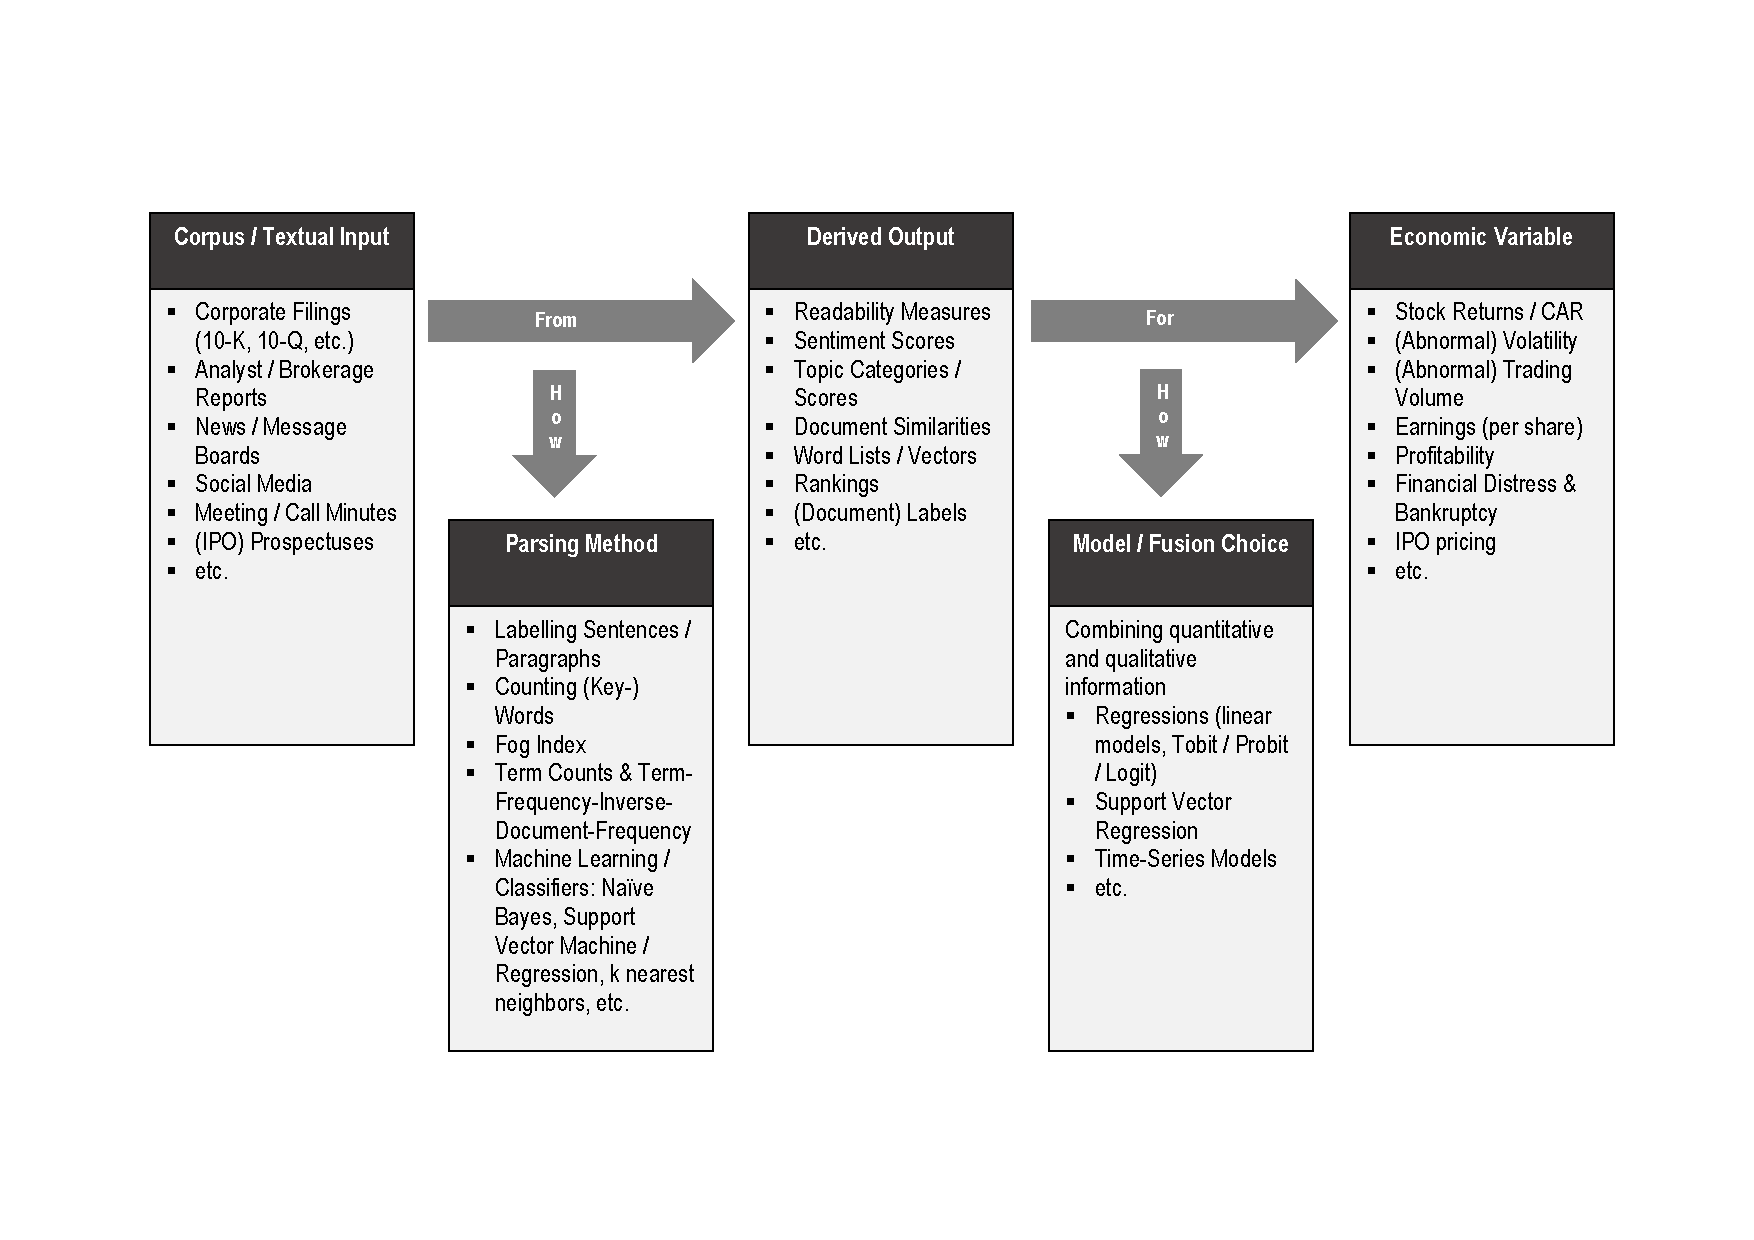
\includegraphics[width=\textwidth]{./Process_graph.pdf}
		\caption{Schematic Representation of a Research Process: Textual Analysis in Finance}
		%\source{Own Representation based on \textcite{LM-meta-2016, Das2014}}
		\label{fig: process_schema}
\end{figure}

\clearpage

% FIGURE
\begin{figure}[H]
	\centering
		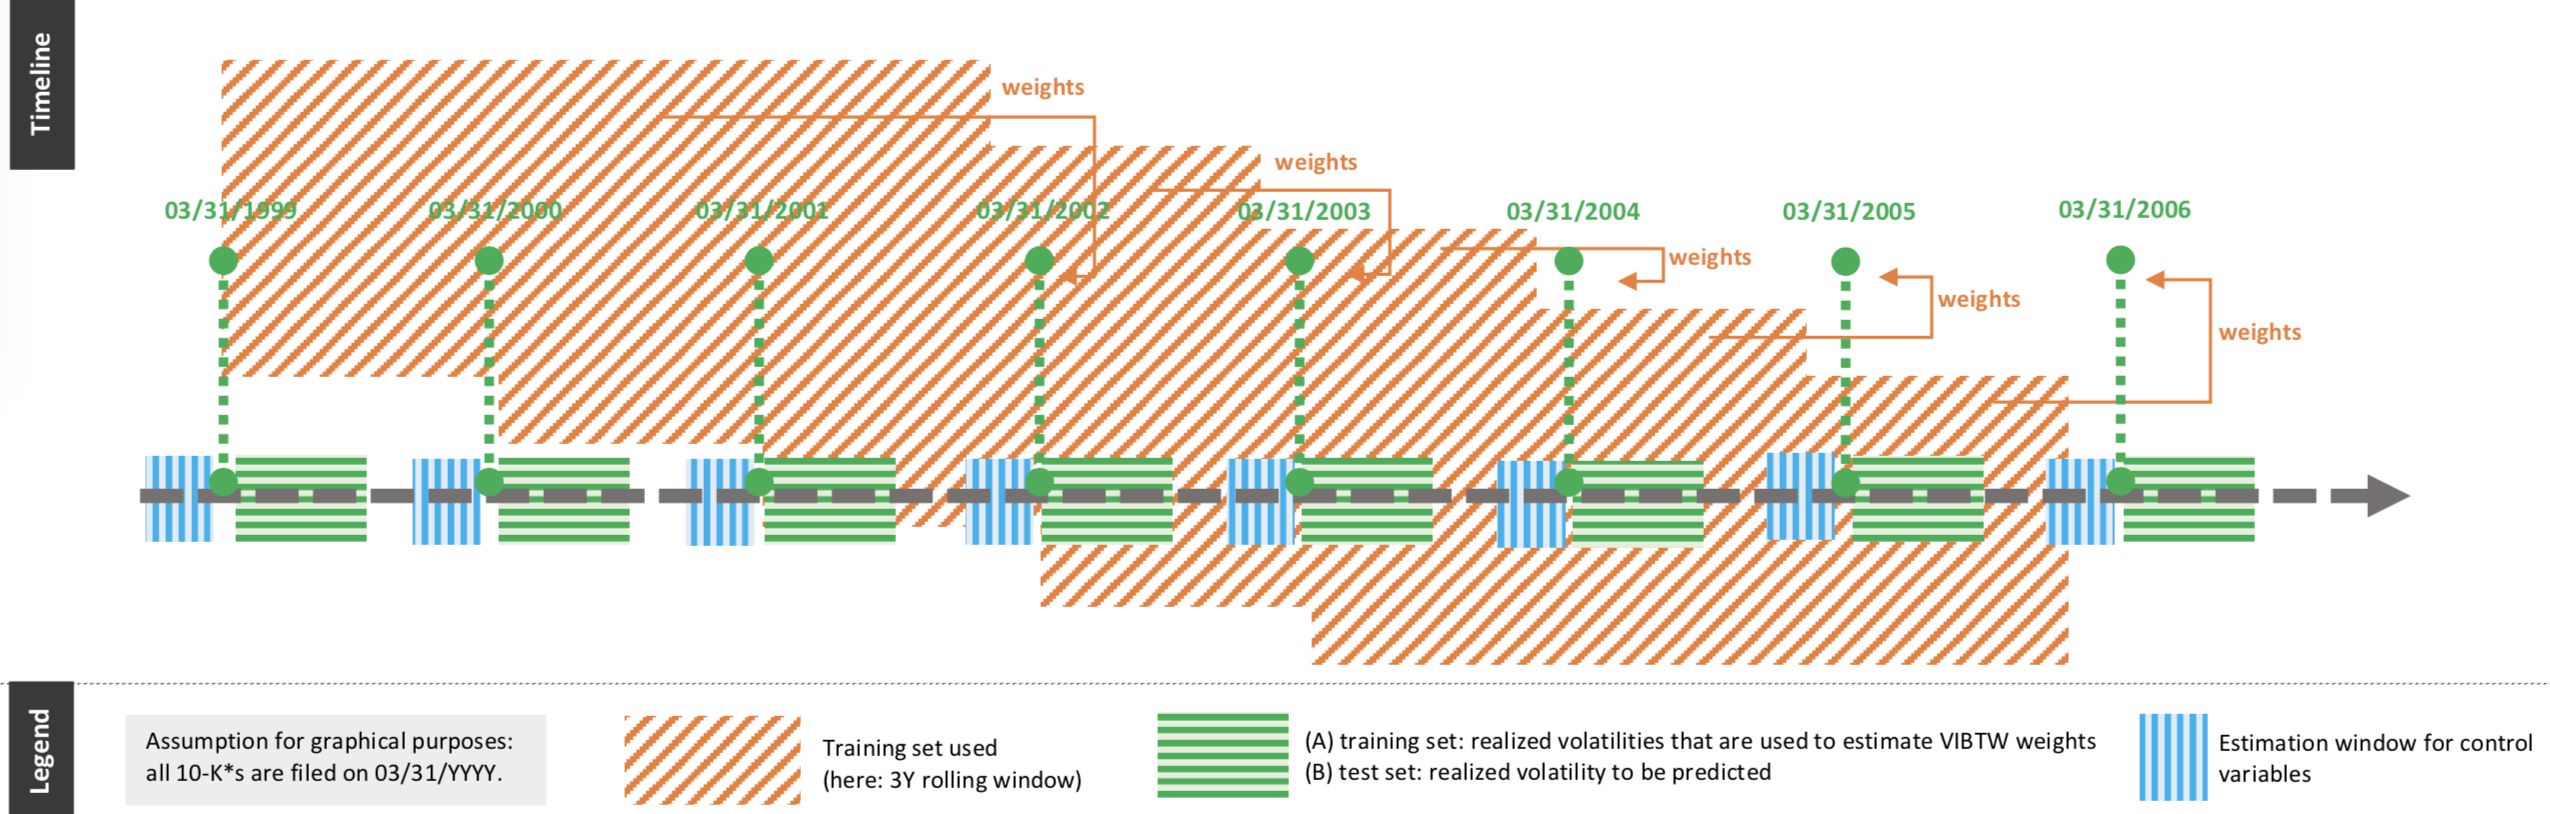
\includegraphics[width=\textwidth]{./timeline_graph}
		\caption{Visualization of the Research Design}
		\label{fig: res_design}
\end{figure}

\clearpage

% FIGURE
\begin{figure}[H]
	\centering
		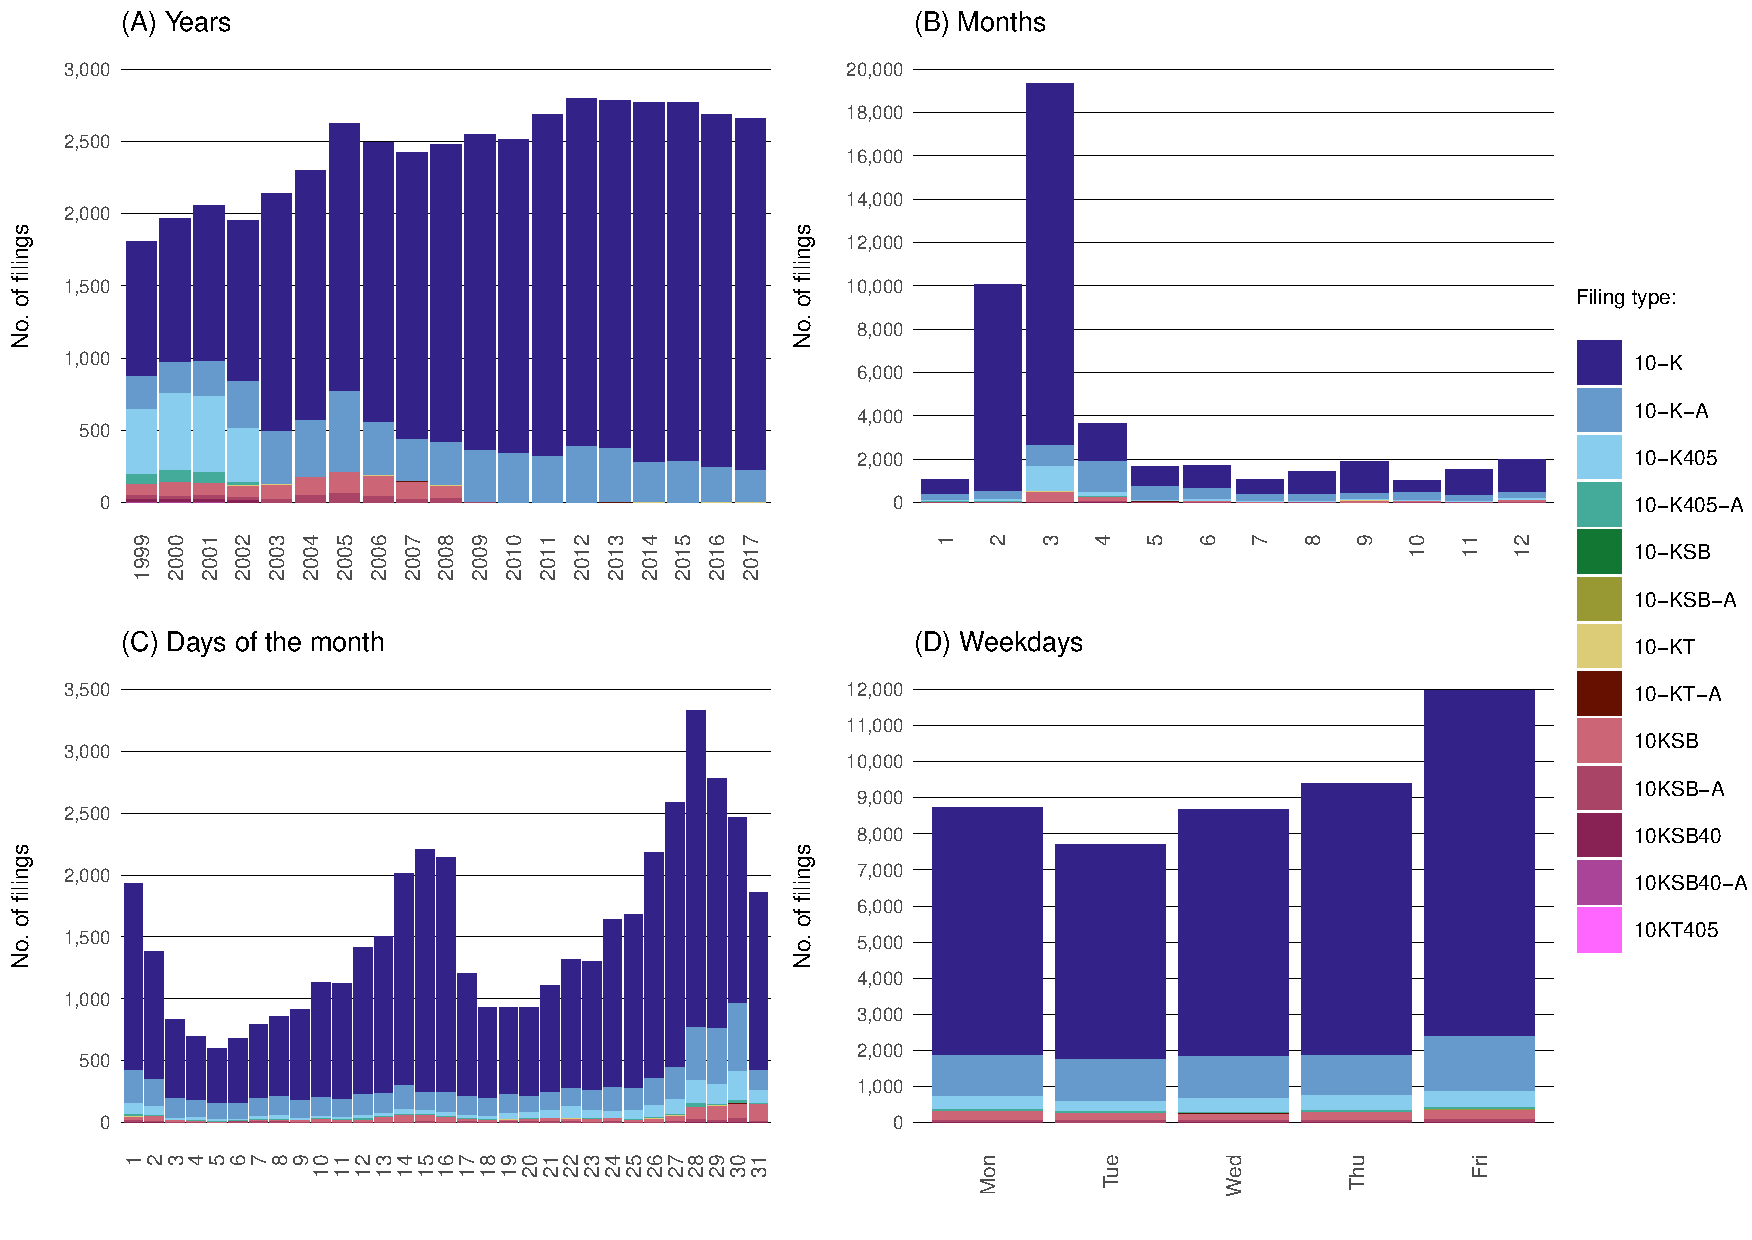
\includegraphics[width=\textwidth]{./no_reports_Y_M_D_type.pdf}
		\caption{Sample Composition by Filing Year, Month, Day, and Type}
		\label{fig: no_reports_ymd_typestacked}
\end{figure}

\clearpage

% FIGURE
\begin{figure}[H]
	\centering
		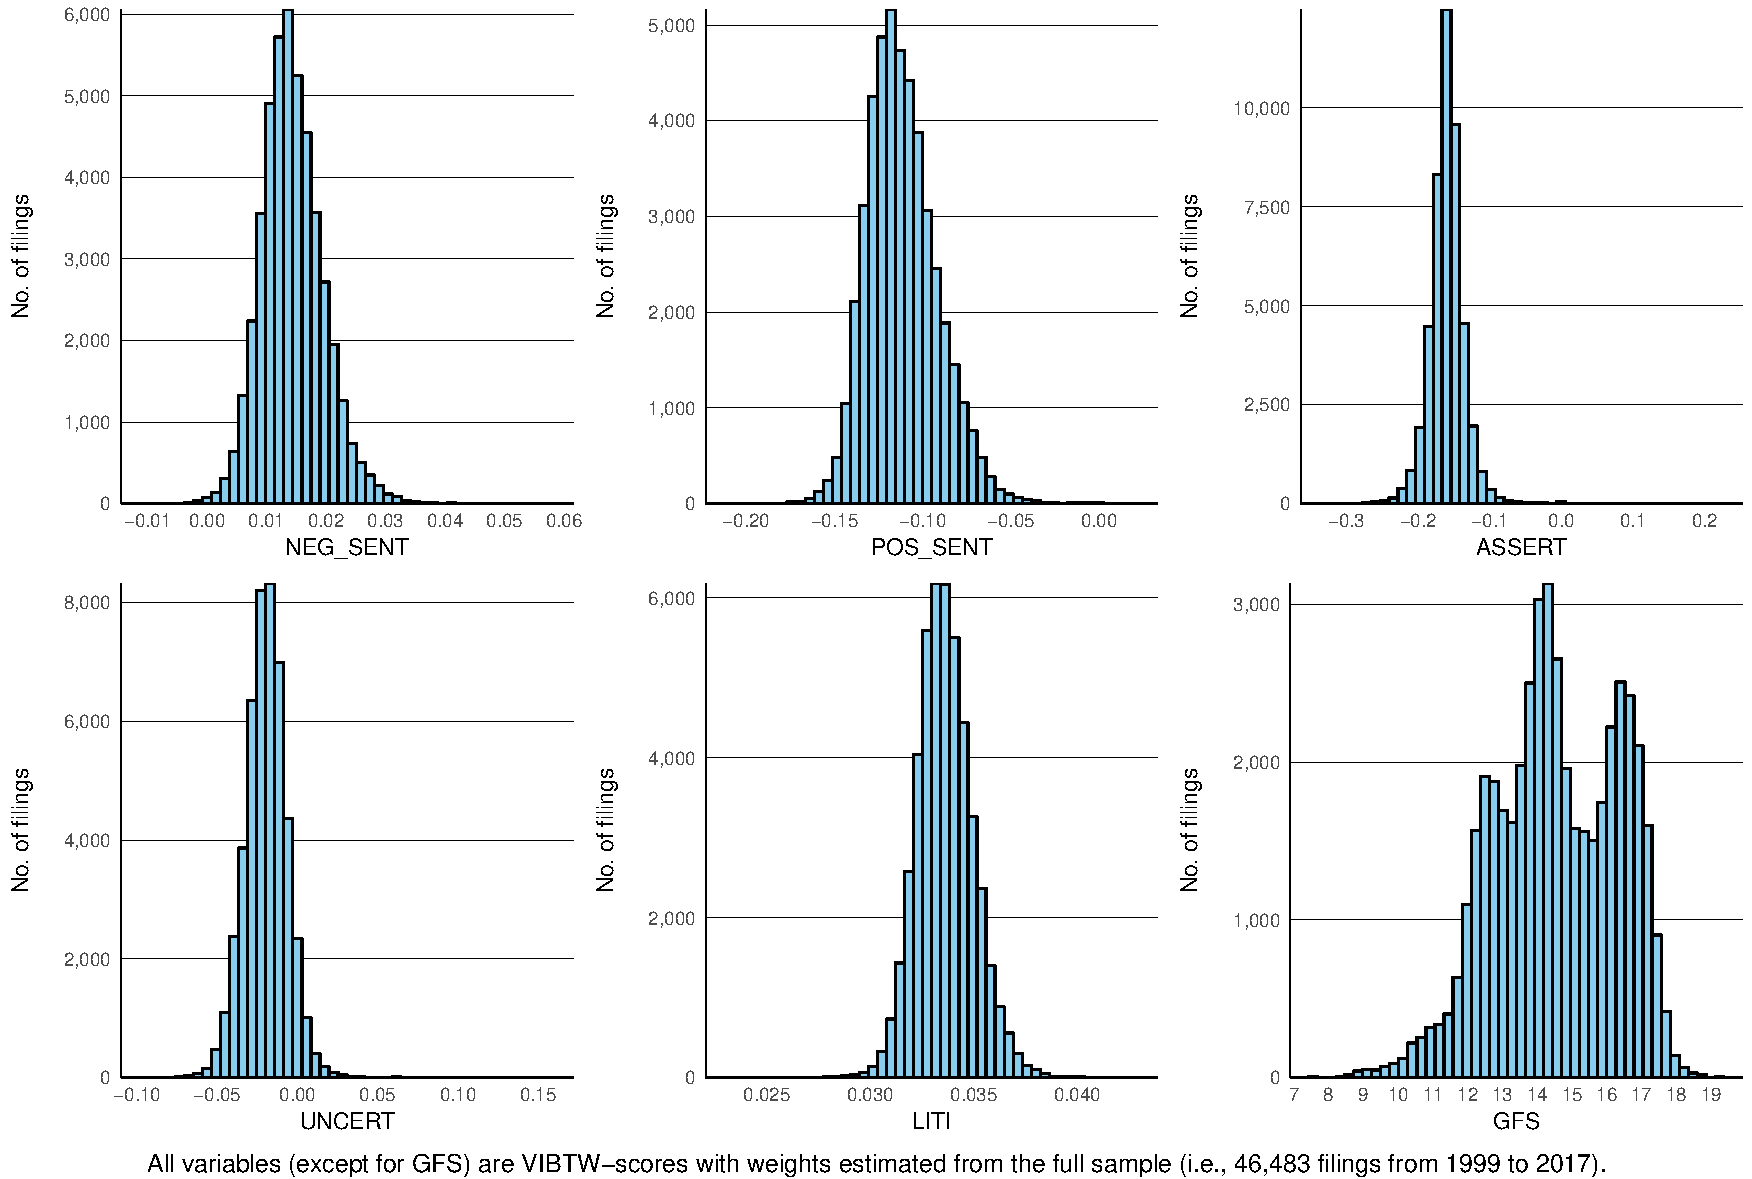
\includegraphics[width=\textwidth]{./histos_LM_scores.pdf}
		\caption{Distribution of Text-Related Variables}
		\label{fig: histos_sentiscores}
\end{figure}

\clearpage

% FIGURE
\begin{figure}[H]
	\centering
		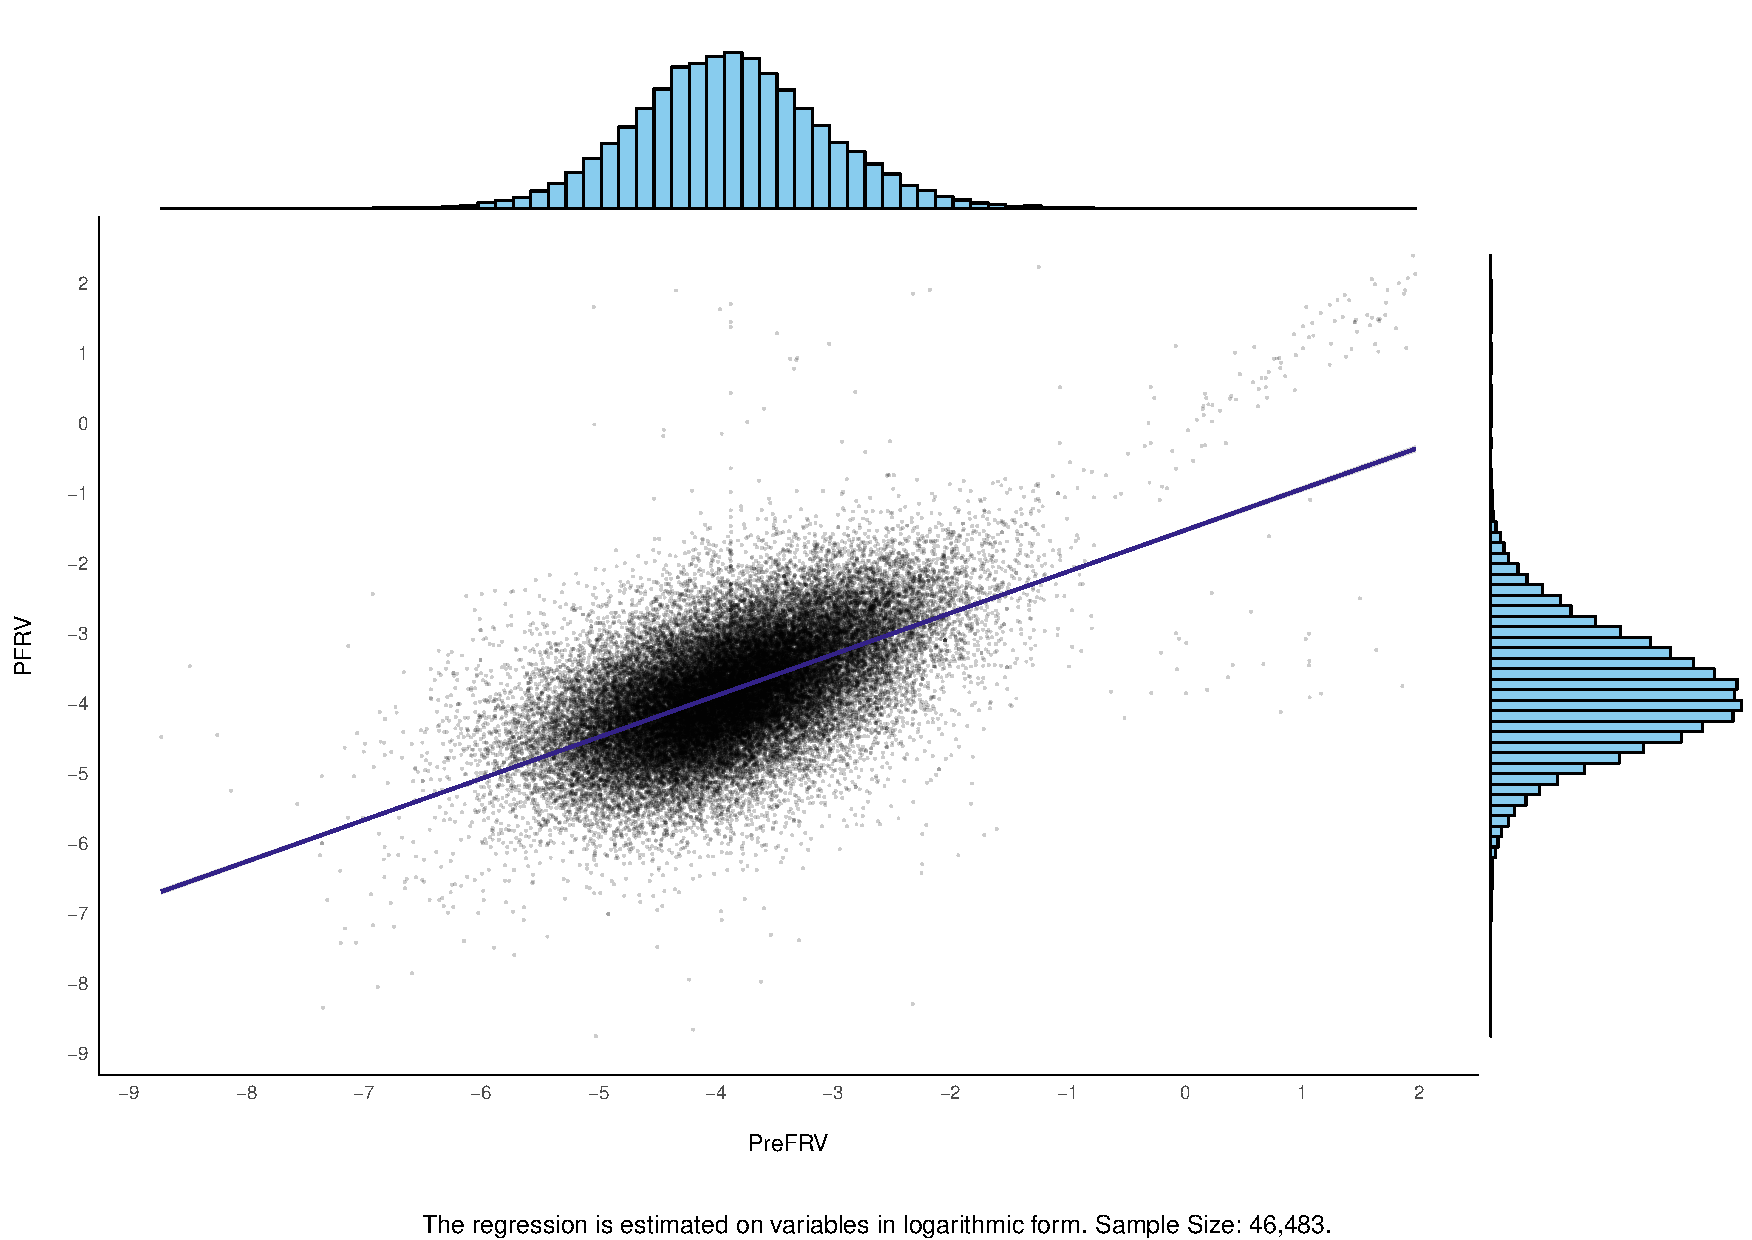
\includegraphics[width=\textwidth]{./MZ_scatter_pre_post.pdf}
		\caption{Post- Versus Pre-Filing Realized Volatility : Scatterplot, Univariate MZ-Regression and Marginal Distributions}
		\label{fig: pfrv_vs_tsfc}
\end{figure}

\clearpage

% FIGURE
\begin{figure}[H]
	\centering
		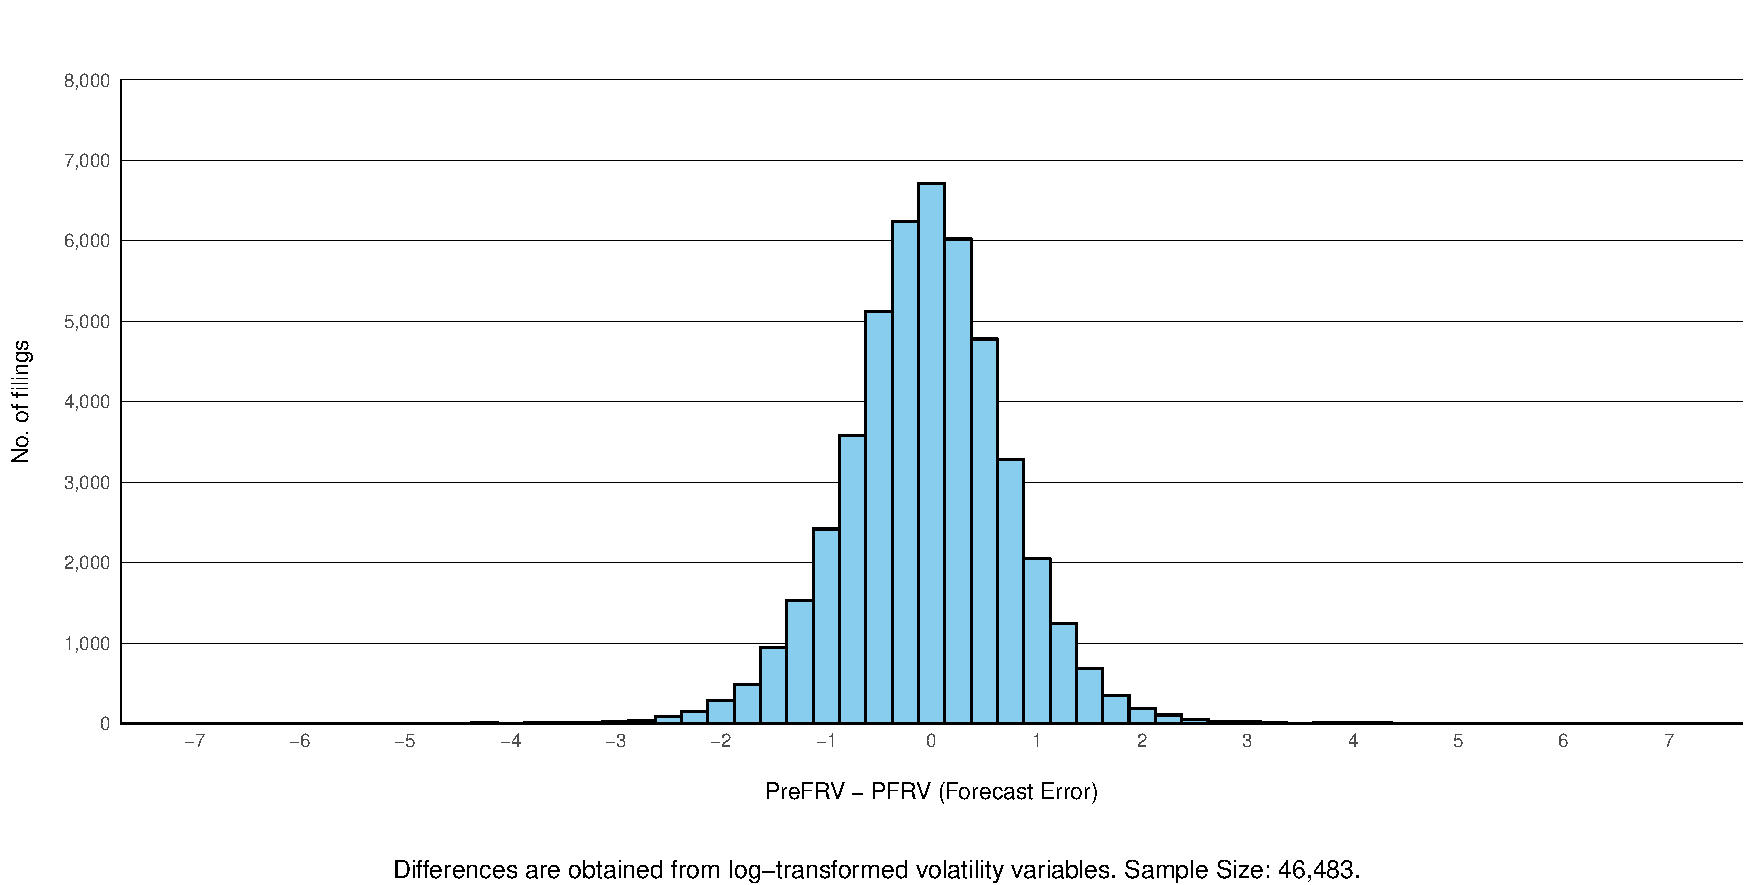
\includegraphics[width=\textwidth]{./delta_pfrv_vs_prefrv.pdf}
		\caption{Post- Versus Pre-Filing Realized Volatility: Forecast Error Distribution}
		\label{fig: delta_histos_pfrv_vs_tsfc}
\end{figure}

\clearpage

%%\processdelayedfloats

%%\makeatletter
%%\efloat@restorefloats
%%\makeatother

\appendix
\section{Appendix}

%%\subsection{Definition of Readability Measures}
%%\label{sec: annex_fogflesch}
%%The following definitions are based on \textcite{Loughran2014}, \textcite{DeFranco2015},  and \textcite{FleschWeb}.
%%
%%The Fog Index is calculated as: 
%%\begin{equation*}
%%0.4 \left[ \dfrac{\text{number of words}}{\text{number of sentences}} + 100 \dfrac{\text{number of complex words}}{\text{number of words}} \right],
%%\end{equation*}
%%where a word is considered complex if it has two or more syllables.
%%
%%The Flesch-Kincaid-Index is calculated as:
%%\begin{equation*}
%%0.39 \left[ \dfrac{\text{number of words}}{\text{number of sentences}} \right] + 11.8 \left[ \dfrac{\text{number of syllables}}{\text{number of words}} \right] - 15.59
%%\end{equation*}
%%
%%The FRES is calculated as:
%%\begin{equation*}
%%206.835 - 1.015 \left[ \dfrac{\text{number of words}}{\text{number of sentences}} \right] + 84.6 \left[ \dfrac{\text{number of syllables}}{\text{number of words}} \right]
%%\end{equation*}
%%
%%Further readability measures, which are less commonly applied in finance and accounting, can be found in \textcite{GuoShiTu2017}. 

\subsection{LM Word Lists}
\label{sec: annex_lm-lists}

The word lists are obtained from \url{https://sraf.nd.edu/textual-analysis/resources/} and are stemmed using the Porter Stemmer, implemented in the \texttt{tm} package in the statistical programming language \texttt{R}. The resulting lexica are composed as follows:

{\scriptsize \textbf{Negative ($J_{N} = 884$):} \textsf{abandon, abdic, aberr, abet, abnorm, abolish, \underline{abrog}, abrupt, absenc, absente, abus, accid, accident, accus, acquiesc, \underline{acquit}, \underline{acquitt}, adulter, adversari, advers, aftermath, against, aggrav, alert, alien, \underline{alleg}, annoy, annul, \underline{anomali}, \underline{anomal}, anticompetit, \underline{antitrust}, argu, argument, \underline{arrearag}, arrear, arrest, artifici, assault, \underline{assert}, attrit, avers, backdat, bad, \underline{bail}, bailout, balk, bankrupt, bankruptci, ban, bar, barrier, bottleneck, boycott, boycot, \underline{breach}, \textit{break}, breakag, breakdown, bribe, briberi, bridg, broken, burden, burdensom, burn, calam, calamit, cancel, careless, catastroph, caution, cautionari, ceas, censur, challeng, chargeoff, circumv, circumvent, \underline{claim}, \underline{clawback}, close, closeout, closur, coerc, coercion, coerciv, collaps, collis, collud, \underline{collus}, \underline{complain}, complaint, complic, \underline{compuls}, conceal, conced, concern, concili, condemn, condon, confess, \underline{confin}, confisc, conflict, confront, confus, conspiraci, conspir, conspiratori, contempt, contend, content, contenti, \underline{contest}, \underline{contract}, contradict, contradictori, contrari, controversi, \underline{convict}, correct, corrupt, cost, counterclaim, counterfeit, countermeasur, \underline{crime}, \underline{crimin}, crise, crisi, critic, crucial, culpabl, cumbersom, curtail, cut, cutback, cyberattack, cyberbulli, cybercrim, cybercrimin, damag, dampen, danger, deadlock, deadweight, debar, deceas, deceit, deceiv, decept, declin, defac, defam, defamatori, default, defeat, \underline{defect}, \underline{defend}, defens, \underline{defer}, defici, deficit, defraud, defunct, degrad, delay, deleteri, deliber, delinqu, delist, demis, demolish, demolit, demot, denial, deni, denigr, deplet, deprec, depress, depriv, derelict, derogatori, \underline{destabil}, destroy, destruct, \underline{detain}, detent, deter, deterior, deterr, detract, detriment, devalu, devast, \underline{deviat}, devolv, difficult, difficulti, diminish, diminut, disadvantag, \underline{disaffili}, disagre, disagr, disallow, disappear, disappoint, disapprov, disassoci, disast, disastr, disavow, disciplinari, disclaim, disclos, discontinu, discourag, discredit, discrep, disfavor, disgorg, disgrac, dishonest, dishonesti, dishonor, disincent, disinterest, disinterested, disloy, disloyalti, dismal, dismiss, disord, disparag, dispar, displac, dispos, \underline{dispossess}, disproport, disproportion, disput, disqualif, disqualifi, disregard, disreput, disrupt, dissatisfact, dissatisfi, dissent, dissid, dissolut, distort, distract, distress, disturb, divers, divert, divest, divestitur, divorc, divulg, \underline{doubt}, downgrad, downsiz, downtim, downturn, downward, drag, drastic, drawback, drop, drought, duress, dysfunct, eas, egregi, embargo, embarrass, embezzl, encroach, \underline{encumb}, \underline{encumbr}, endang, endanger, enjoin, erod, eros, errat, \textit{er}, erron, error, err, escal, evad, evas, evict, exacerb, exagger, excess, \underline{exculp}, \underline{exculpatori}, exoner, exploit, expos, expropri, expuls, extenu, fail, failur, fallout, fals, falsif, falsifi, falsiti, fatal, fault, faulti, fear, \underline{feloni}, fictiti, fine, fire, flaw, \underline{forbid}, \underline{forbidden}, forc, foreclos, foreclosur, forego, foregon, forestal, \underline{forfeit}, forfeitur, forger, forgeri, fraud, fraudul, frivol, frustrat, \underline{fugit}, gratuit, grievanc, grossli, groundless, guilti, halt, hamper, harass, hardship, harm, harsh, harsher, harshest, hazard, hinder, hindranc, hostil, hurt, idl, ignor, ill, illeg, illicit, illiquid, imbal, immatur, immor, \underline{impair}, impass, imped, impedi, impend, imper, imperfect, imperil, impermiss, implic, imposs, impound, impractic, impract, imprison, improp, improprieti, imprud, inabl, inaccess, inaccuraci, inaccur, inact, inactiv, inadequaci, inadequ, inadvert, inadvis, inappropri, inattent, incap, incapacit, \underline{incapac}, \underline{incarcer}, incid, incompat, incompet, \underline{incomplet}, inconclus, inconsist, inconveni, incorrect, indec, indefeas, \underline{indict}, ineffect, ineffici, inelig, inequit, inequ, inevit, inexperi, inexperienc, inferior, inflict, \underline{infract}, \underline{infring}, \underline{inhibit}, inim, injunct, injur, injuri, inordin, inquiri, insecur, insensit, insolv, \underline{instabl}, insubordin, insuffici, insurrect, intent, interfer, interf, intermitt, interrupt, intimid, intrus, invalid, investig, involuntarili, involuntari, irreconcil, irrecover, irregular, irrepar, irrevers, jeopard, justifi, kickback, know, lack, lacklust, lag, laps, late, launder, layoff, lie, \underline{limit}, linger, liquid, \underline{litig}, lockout, lose, loss, lost, malfeas, malfunct, malic, malici, malpractic, manipul, markdown, misappl, misappli, misappropri, misbrand, miscalcul, mischaracter, mischief, misclassif, misclassifi, miscommun, misconduct, misdat, \underline{misdemeanor}, misdirect, mishandl, misinform, misinterpret, misjudg, mislabel, mislead, misl, mismanag, mismatch, misplac, mispric, misrepres, misrepresent, miss, misstat, misstep, mistak, mistaken, \underline{mistrial}, misunderstand, misunderstood, misus, monopolist, monopol, monopoli, moratoria, moratorium, mothbal, negat, neglect, neglig, nonattain, noncompetit, noncompli, nonconform, nondisclosur, nonfunct, nonpay, nonperform, nonproduc, nonproduct, nonrecover, nonrenew, nuisanc, \underline{nullif}, \underline{nullifi}, object, objection, obscen, obsolesc, obsolet, obstacl, obstruct, offenc, offend, omiss, omit, oner, opportunist, oppos, opposit, outag, outdat, outmod, overag, overbuild, overbuilt, overburden, overcapac, overcharg, overcom, overdu, overestim, overload, overlook, overpaid, overpay, overproduc, overproduct, overrun, overshadow, overst, overstat, oversuppli, overt, overturn, overvalu, panic, penal, penalti, peril, \underline{perjuri}, \underline{perpetr}, persist, pervas, petti, picket, \underline{plaintiff}, \underline{plea}, \underline{plead}, pled, poor, pose, postpon, precipit, \underline{preclud}, predatori, prejudic, \underline{prejud}, \underline{prejudici}, prematur, press, \underline{pretrial}, \underline{prevent}, problem, problemat, prolong, prone, \underline{prosecut}, protest, protestor, protract, provok, \underline{punish}, punit, purport, question, quit, racket, ration, \underline{reassess}, reassign, recal, recess, recessionari, reckless, \underline{redact}, redefault, redress, refus, reject, relinquish, reluct, renegoti, renounc, repar, repossess, repudi, resign, restat, restructur, retali, retaliatori, retribut, \underline{revoc}, revok, ridicul, \underline{riskier}, \underline{riskiest}, \underline{riski}, sabotag, sacrific, sacrif, sacrifici, scandal, scrutin, scrutini, secreci, seiz, \underline{sentenc}, serious, setback, \underline{sever}, sharpli, shock, shortag, shortfal, shrinkag, shut, shutdown, slander, slippag, slow, slowdown, slower, slowest, slowli, sluggish, solvenc, spam, spammer, stagger, stagnant, stagnat, standstil, stolen, stoppag, stop, strain, stress, stringent, subject, \underline{subpoena}, substandard, \underline{sue}, \underline{\textit{su}}, suffer, \underline{summon}, \underline{summons}, \underline{suscept}, suspect, suspend, suspens, suspicion, suspici, taint, tamper, tens, \underline{termin}, \underline{testifi}, threat, threaten, tighten, toler, tortuous, tragedi, tragic, traumat, troubl, \underline{turbul}, turmoil, unabl, unaccept, unaccount, unannounc, unanticip, unapprov, unattract, unauthor, \underline{unavail}, unavoid, unawar, uncollect, uncompetit, uncomplet, unconscion, uncontrol, uncorrect, uncov, undeliver, undeliv, undercapit, undercut, underestim, underfund, underinsur, undermin, underpaid, underpay, underperform, underproduc, underproduct, underreport, underst, understat, underutil, undesir, \underline{undetect}, \underline{undetermin}, undisclos, \underline{undocu}, undu, unduli, uneconom, unemploy, uneth, unexcus, \underline{unexpect}, unfair, unfavor, unfavour, unfeas, unfit, unforese, unforeseen, \underline{unforseen}, unfortun, unfound, unfriend, unfulfil, unfund, uninsur, unintend, unintent, unjust, unjustifi, unknow, \underline{unlaw}, unlicens, unliquid, unmarket, unmerchant, unmeritori, unnecessarili, unnecessari, unneed, unobtain, unoccupi, unpaid, unperform, \underline{unplan}, unpopular, \underline{unpredict}, unproduct, unprofit, unqualifi, unrealist, unreason, unrecept, unrecover, unrecov, unreimburs, unreli, \underline{unremedi}, unreport, unresolv, unrest, unsaf, unsal, unsatisfactori, unsatisfi, unsavori, unschedul, unsel, unsold, unsound, unstabil, unstabl, unsubstanti, unsuccess, unsuit, unsur, unsuspect, unsustain, unten, untim, untrust, untruth, unus, unwant, unwarr, unwelcom, unwil, unwilling, upset, urgenc, urgent, \underline{usuri}, \underline{usurp}, vandal, \underline{verdict}, veto, victim, \underline{violat}, violenc, violent, vitiat, \underline{void}, \underline{volatil}, vulner, warn, wast, weak, weaken, weaker, weakest, \underline{will}, worri, wors, worsen, worst, worthless, writedown, writeoff, wrong, wrongdo}

\textbf{Positive ($J_{P} = 145$):} \textsf{abl, abund, acclaim, accomplish, achiev, adequ, advanc, advantag, allianc, assur, attain, attract, beauti, \underline{benefici}, benefit, \underline{best}, better, bolster, boom, boost, breakthrough, brilliant, charit, collabor, compliment, complimentari, conclus, conduc, confid, construct, courteous, creativ, delight, \underline{depend}, desir, despit, destin, dilig, distinct, dream, easier, easili, easi, effect, effici, empow, enabl, encourag, enhanc, enjoy, enthusiasm, enthusiast, excel, except, excit, exclus, exemplari, fantast, favor, favorit, friend, gain, good, great, greater, greatest, happiest, happili, happi, \underline{highest}, honor, ideal, impress, improv, incred, influenti, inform, ingenu, innov, insight, inspir, integr, invent, inventor, leadership, lead, loyal, lucrat, meritori, opportun, optimist, outperform, perfect, pleasant, pleas, pleasur, plenti, popular, posit, preemin, premier, prestig, prestigi, proactiv, profici, profit, progress, prosper, rebound, recept, regain, resolv, revolution, reward, satisfact, satisfactorili, satisfactori, satisfi, smooth, solv, spectacular, stabil, stabl, strength, strengthen, \underline{strong}, stronger, strongest, succeed, success, superior, surpass, transpar, tremend, unmatch, \underline{unparallel}, \underline{unsurpass}, upturn, valuabl, versatil, vibranc, vibrant, win, winner, worthi}

\textbf{Uncertainty ($J_{U} = 129$):} \textsf{abey, \underline{almost}, alter, ambigu, \underline{anomali}, \underline{anomal}, anticip, \underline{appar}, \underline{appear}, approxim, arbitrarili, arbitrari, \underline{assum}, assumpt, believ, cautious, clarif, \underline{conceiv}, condit, \underline{confus}, conting, \underline{could}, crossroad, \underline{depend}, \underline{destabil}, \underline{deviat}, differ, \underline{doubt}, exposur, fluctuat, hidden, hing, imprecis, improb, \underline{incomplet}, indefinit, indetermin, inexact, \underline{instabl}, intang, likelihood, \underline{may}, \underline{mayb}, \underline{might}, \underline{near}, nonassess, \underline{occasion}, ordinarili, pend, \underline{perhap}, \underline{possibl}, precaut, precautionari, predict, predictor, preliminarili, preliminari, presum, presumpt, probabilist, \underline{probabl}, random, \underline{reassess}, recalcul, reconsid, reexamin, reinterpret, revis, risk, \underline{riskier}, \underline{riskiest}, \underline{riski}, rough, rumor, seem, \underline{seldom}, \underline{sometim}, \underline{somewhat}, somewher, specul, sporad, sudden, \underline{suggest}, \underline{suscept}, \underline{tend}, tentat, \underline{turbul}, \underline{uncertain}, uncertainti, unclear, unconfirm, undecid, undefin, undesign, \underline{undetect}, \underline{undetermin}, \underline{undocu}, \underline{unexpect}, unfamiliar, unforecast, unforseen, unguarante, unhedg, unidentifi, unknown, unobserv, \underline{unplan}, \underline{unpredict}, unprov, unproven, unquantifi, unreconcil, unseason, unsettl, unspecif, unspecifi, untest, unusu, unwritten, vagari, vagu, \textit{vaguer}, \textit{vaguest}, variabl, varianc, variant, variat, vari, \underline{volatil}}

\textbf{Litigious ($J_{L} = 451$):} \textsf{abovement, \underline{abrog}, absolv, access, acquire, acquiror, \underline{acquit}, \underline{acquitt}, addendum, adjourn, adjudg, adjud, adjudicatori, admiss, affidavit, affirm, affreight, aforedescrib, aforement, aforesaid, aforest, aggriev, \underline{alleg}, amend, amendatori, anteced, anticorrupt, \underline{antitrust}, anywis, appeal, appel, appelle, appointor, appurten, arbitr, \underline{arrearag}, ascend, \underline{assert}, assign, \underline{assum}, attest, attorn, attorney, \underline{bail}, baile, bailiff, bailment, \underline{benefici}, bona, bonafid, \underline{breach}, cedant, certiorari, cession, chattel, choat, \underline{claim}, claimabl, claimant, claimhold, \underline{clawback}, codefend, codicil, codif, codifi, \underline{collus}, compensatori, \underline{complain}, condemnor, confiscatori, consent, conservatorship, constitut, constru, \underline{contest}, \underline{contract}, contracthold, contractil, contractu, contraven, contravent, controvert, convenien, convey, \underline{convict}, cotermin, counsel, \textit{countersignor}, countersu, countersuit, court, courtroom, \underline{crime}, \underline{crimin}, crossclaim, deced, declar, decre, defalc, defeas, \underline{defect}, \underline{defend}, \underline{defer}, deleg, delegat, delegate, delege, demur, demurr, depos, deposit, derog, design, desist, \underline{detain}, devise, \underline{disaffili}, disaffirm, disposit, \underline{dispossess}, dispossessori, distraint, distribute, docket, done, duli, eject, \underline{encumb}, \underline{encumbr}, encumbranc, endorse, enforc, escheat, \underline{escrow}, estoppel, evidenti, evidentiari, exceed, excis, \underline{exculp}, \underline{exculpatori}, executor, executori, \textit{executric}, executrix, extracontractu, extracorpor, extrajudici, faci, facto, \underline{feloni}, fide, \underline{\textit{forbad}}, forbear, forebear, \underline{forfeit}, forthwith, \textit{forwhich}, \underline{fugit}, further, grantor, henceforth, henceforward, hereaft, herebi, heredita, herefor, herefrom, herein, hereinabov, hereinaft, hereinbefor, hereinbelow, hereof, hereon, hereto, heretofor, hereund, hereunto, hereupon, herewith, herewithin, immateri, implead, inasmuch, \underline{incapac}, \underline{incarcer}, inchoat, incontest, indemnifi, indemnif, indemnite, indemn, indemnitor, \underline{indict}, indorse, inforc, \underline{infract}, \underline{infring}, \underline{injunct}, insofar, interlocutori, interplead, interpos, interposit, interrog, interrogatori, intestaci, intest, \underline{irrevoc}, joinder, judici, judiciari, juri, jurisdict, jurisprud, jurist, juror, \textit{juryman}, justic, law, lawmak, lawsuit, lawyer, legal, legales, legate, legisl, legislatur, libel, licens, lienhold, \underline{litig}, litigi, \textit{majeur}, mandamus, mediat, \underline{misdemeanor}, misfeas, \underline{mistrial}, moreov, motion, mutandi, nolo, nonappeal, nonbreach, nonconting, noncontract, noncontractu, noncontributori, nonfeas, nonfiduciari, nonforfeit, nonforfeitur, nonguarantor, noninfring, nonjudici, nonjurisdict, nonsever, nontermin, nonusuri, notari, notar, notwithstand, novo, \underline{nullif}, \underline{nullifi}, nulliti, oblige, obligor, offens, offere, offeror, optione, overrul, para, pari, passu, patente, pecuniarili, \underline{perjuri}, permitte, \underline{perpetr}, personam, petit, petition, \underline{plaintiff}, \underline{plead}, \underline{plea}, pledge, pledgor, possessori, postclos, postclosur, postcontract, postjudg, preamend, predeceas, prehear, \underline{prejudic}, \underline{prejud}, \underline{prejudici}, prepetit, \underline{presumpt}, \underline{pretrial}, prima, priviti, probat, probationari, \textit{probation}, promulg, prorata, prorat, \underline{prosecut}, prosecutor, prosecutori, proviso, \underline{punish}, quitclaim, rata, ratabl, reargument, rebut, rebutt, record, recoup, recours, rectif, recus, \underline{redact}, referenda, referendum, refil, regul, regulatori, rehear, reheard, release, remand, remedi, remis, repledg, replevin, request, requestor, reregul, rescind, resciss, restitutionari, retend, retroced, retrocessionair, \underline{revoc}, rule, \underline{sentenc}, sequestr, settlement, \underline{sever}, shall, statut, statutorili, statutori, subclaus, subdocket, sublease, subleasehold, sublessor, sublicense, sublicensor, subparagraph, \underline{subpoena}, subrog, subtrust, \underline{sue}, \underline{\textit{su}}, \underline{summon}, \underline{summons}, supersed, supersedea, sureti, tenant, \underline{termin}, terminus, testamentari, \underline{testifi}, testimoni, thenc, thenceforth, \textit{thenceforward}, thereaft, thereat, therefrom, therein, thereinaft, thereof, thereon, thereov, thereto, theretofor, thereund, thereunto, thereupon, therewith, tort, tortious, transferor, unappeal, unapp, unconstitut, uncontract, undefeas, undischarg, unencumb, unenforc, \underline{unlaw}, \underline{unremedi}, unstay, unto, \underline{usuri}, \underline{usurp}, vende, \underline{verdict}, viatic, \underline{violat}, voidabl, \underline{void}, warrante, warrantor, whatev, whatsoev, whensoev, whereabout, wherea, whereat, wherebi, wherefor, wherein, whereof, whereon, whereto, whereund, whereupon, wherewith, whistleblow, whomev, whomsoev, whosoev, wil, \underline{will}, wit, writ}

\textbf{Constraining ($J_{C} = 57$):} \textsf{abid, bound, commit, compel, compli, \underline{compuls}, compulsori, \underline{confin}, constrain, constraint, coven, \underline{depend}, dictat, direct, earmark, \underline{encumb}, \underline{encumbr}, entail, entrench, \underline{escrow}, \underline{\textit{forbad}}, \underline{forbid}, forbidden, \underline{impair}, impos, imposit, indebt, \underline{inhibit}, insist, \underline{irrevoc}, \underline{limit}, mandat, mandatori, manditorili, necessit, noncancel, oblig, obligatori, permiss, permit, pledg, \underline{preclud}, precondit, preset, \underline{prevent}, prohibit, prohibitori, refrain, requir, restrain, restraint, restrict, stipul, strict, stricter, strictest, \underline{unavail}}

\textbf{Strong Modal ($J_{SM} = 17$):} \textsf{alway, \underline{best}, clear, definit, \underline{highest}, lowest, must, never, \underline{strong}, unambigu, uncompromis, undisput, undoubt, unequivoc, \underline{unparallel}, \underline{unsurpass}, \underline{will}}

\textbf{Modest Modal ($J_{MM} = 13$):} \textsf{can, frequent, general, like, often, ought, \underline{probabl}, rare, regular, should, \underline{tend}, usual, would}

\textbf{Weak Modal ($J_{WM} = 18$):} \textsf{\underline{almost}, \underline{appar}, \underline{appear}, \underline{conceiv}, \underline{could}, \underline{depend}, \underline{may}, \underline{mayb}, \underline{might}, \underline{near}, \underline{occasion}, \underline{perhap}, \underline{possibl}, \underline{seldom}, \underline{sometim}, \underline{somewhat}, \underline{suggest}, \underline{uncertain}}}

This gives a total of 1,714 stemmed words; while due to overlapping in the lists, there are 1,574 \textit{unique} words. The 140 words that appear in more than one list are underlined. 15 words (13 unique types) out of this list do not appear in any of the 46,483 10-K* documents of the corpus; they are printed in italic font. Details about the composition of LM lists and their respective size after stemming and searching for them in the corpus are provided in Table \ref{tab: LM_lexicon}. 

\clearpage

% TABLE
\input{./Results_Tables/sumstats_LM_lexicon_final}

%%\subsection{Time-Series Models}
%%\label{sec: annex_garch_gjr}
%%
%%In this thesis, GARCH and GJR-GARCH were used as time-series inputs in MZ-regressions in the robustness checks. This section gives a brief theoretical explanation about these two models.
%%
%%\nomenclature{GARCH}{Generalized Auto-Regressive Conditional Heteroskedasticity}
%%\nomenclature{ARCH}{Auto-Regressive Conditional Heteroskedasticity}
%%\nomenclature{ARMA}{Auto-Regressive Moving-Average (Process)}
%%\nomenclature{GJR-GARCH}{GARCH-model developed by \textcite{GJR1993}}
%%
%%The GARCH model was introduced by \textcite{Bollerslev1986}, who extended the ARCH model developed by \textcite{Engle1982}. This was achieved by modelling volatility in a fashion that corresponds to an \enquote{ARMA-like} specification rather than an \enquote{AR-like}; in this line of thought, ARCH(q) can be interpreted as an AR(q) model of the \textbf{squared innovations} of the return series, whereas the GARCH(p,q) model can be seen as an ARMA(q,p) model of the \textbf{squared innovations}\footnote{This notation actually refers to the \textbf{squared innovations}, as, in contrast, when looking at the conditional variance equation, the \enquote{new part} in GARCH is actually the auto-regressive structure that was achieved by adding lags of $\sigma_t^2$ itself. Conversely, the conditional variance in ARCH itself was a \textbf{moving-average} process - but \textcite{Engle1982} was referring to squared residuals when specifying it as an AR-model. Therefore, the number of auto-regressive terms ($q$) in GARCH usually refers to the lags of $e_t$ included, as was the case for the general ARCH (and which is the reason why it is called \enquote{auto-regressive} or \enquote{ARCH}-part). Thus, $p$ relates to the lags of $\sigma_t^2$ included and is called \enquote{moving-average} or \enquote{GARCH}-part (although the strong focus on the conditional variance equation would possibly give the inclination to think of it vice versa and can lead to some confusion).}.
%%The basic model with one lag for both the auto-regressive and moving-average terms (i.e., $q=p=1$) reads as follows:
%%\begin{align*}
%%\text{GARCH(1,1): }\qquad & r_t = \mu_{t} + e_{t}, \quad e_{t} = \sigma_{t} z_{t},\quad  z_{t} \overset{\text{iid}}{\sim} \mathcal{G}(0,1) \\
%%& \sigma_t^2 = \alpha_0 + \alpha_1 \cdot e_{t-1}^2 + \beta_1 \cdot \sigma_{t-1}^2, \label{eq: GARCH} \numberthis
%%\end{align*}
%%
%%where $r_t$ is the time series of continuously compounded asset returns and $\mu_{t} = \expect{r_t|\mathcal{F}_{t-1}}$ is the conditional mean series\footnote{It is called \emph{conditional} because it depends on the information set available in $t-1$, which is denoted by $\mathcal{F}_{t-1}$.}. Very often one assumes $\mu_{t}$ to be constant over time ($ \mu_{t}=\mu $), or even zero ($ \mu_{t}=\mu=0 $). The latter was also assumed in the thesis in hand. Otherwise, the conditional mean series usually is described by some simple process out of the ARMA family.
%%Furthermore, in terms of notation, the series $e_t$ is referred to as \enquote{innovation process}, whilst also \enquote{shock}, \enquote{error} or \enquote{residual} of the return series (with respect to the mean process $\mu_t$) are often used terminology. It is described as the white noise process $z_t$ scaled by $\sigma_{t}^2 = Var[r_t | \mathcal{F}_{t-1} ]$. The latter is called the (squared) \textbf{volatility} of the return series. Note that $z_t$, as said, is strong white noise, i.e., a zero-centred, unit-variance series that it is \textit{i.i.d.} according to some generic distribution $\mathcal{G}$\footnote{In practice, the most common choices for $\mathcal{G}$ are the standard normal as well as the Student t distribution. In this thesis, the standard normal was the distribution of choice.}. Moreover, one imposes that $z_t$ is independent of $\mathcal{F}_{t-1}$.
%%
%%It shall once more be noted that equation \eqref{eq: GARCH} is concerned with the modelling of \textbf{conditional} variance, which is a random variable depending on the information set of \enquote{past returns}, which was denoted by $\mathcal{F}_{t-1}$. Note that GARCH as a generalization of ARCH also nests the latter model (with the special case of $p = 0$). Moreover, by substituting the lags of $\sigma^2$ recursively, one can show that a simple GARCH(1,1) actually is equivalent to a ARCH($\infty$) making the predictive power similar to higher-order ARCH processes while being much more parsimonious with the number of parameters to be estimated, and, thus, making it computationally more attractive compared to ARCHs with lots of lags. 
%%
%%It is worth mentioning that in the GARCH(p,q) one typically imposes so-called stationarity conditions, so as to ensure the \textit{unconditional} variance to be finite. The stationarity restricts the coefficients as follows: $\sum_{i=1}^q \alpha_i + \sum_{i=1}^p \beta_i  < 1$. This is because the unconditional variance is defined as: 
%%\begin{equation}
%%\label{eq: lt-variance-GARCH}
%%Var[e_t] = \expect{e_t^2} = \dfrac{\alpha_0}{1- \sum_{i=1}^q \alpha_i + \sum_{i=1}^p \beta_i}
%%\end{equation}
%%
%%Using the definition of unconditional variance in equation \eqref{eq: lt-variance-GARCH} and denoting $Var[e_t] \coloneqq \bar{\sigma}^2$ one can find $k$-period ahead forecasts for the GARCH(1,1): $\hat{\sigma}_{h+k}^2 = \alpha_0 + (\alpha_1 + \beta_1) \hat{\sigma}_{h+k-1}^2 = \bar{\sigma}^2 + (\alpha_1 + \beta_1)^k (\sigma_t^2 - \bar{\sigma}^2)$. The last part of the equation clearly undermines the mean-reversion \enquote{towards} the unconditional variance, $\bar{\sigma}^2$, as $(\alpha_1 + \beta_1)^k$ will converge to zero for large $k$ due to the fact that $(\alpha_1 + \beta_1) < 1$, which is guaranteed by imposing the usual stationarity conditions. In this context, \textcite[8]{Engle2001} points out: 
%%\blockquote{Although this model is directly set up to forecast for just one period, it turns out that based on the one period forecast a two period forecast can be made. Ultimately by repeating this step, long horizon forecasts can be constructed. For the GARCH(1,1) the two step forecast is a little closer to the long run average variance than the one step forecast and ultimately, the distant horizon forecast is the same for all time periods as long as $\alpha + \beta < 1$. This is just the unconditional variance. Thus the GARCH models are mean reverting and conditionally heteroskedastic but have a constant unconditional variance.}
%%
%%In the course of time, the basic specification of the GARCH process has been further extended so as to capture further stylized facts about financial return time series. The most prominent developments on the model are designed in order to account for the so-called \enquote{leverage effect}. This empirical property of return series makes a statement about asymmetries in volatility modelling, namely that negative returns increase the conditional volatility by a larger amount than positive counterparts of equal magnitude do. 
%%
%%One model that is able to capture asymmetry in conditional variance is the GARCH extension by \textcite{GJR1993}. By the initial letters of the authors' names this model is called GJR-GARCH. The model is able to capture the leverage effect \enquote{by allowing \textelp{} positive and negative innovations to returns having different impacts on conditional volatility} \parencite[1779]{GJR1993}. The model can be written as follows:
%%\begin{align*}
%%\text{GJR-GARCH(1,1): }\qquad &  r_t = \mu_{t} + e_{t}, \quad e_{t} = \sigma_{t} z_{t},\quad  z_{t} \overset{\text{iid}}{\sim} \mathcal{G}(0,1) \\
%%& \sigma_t^2 = \alpha_0 + \alpha_1 \cdot e_{t-1}^2 + \xi_1 \cdot e_{t-1}^2 \cdot I_{[e_{t-1}<0]} + \beta_1 \cdot \sigma_{t-1}^2, \numberthis
%%\end{align*} 
%%where $I_{[e_{t-1}<0]}$ follows the usual definition; it is an indicator variable that equals one whenever $e_{t-1}<0$ and zero otherwise. Using that simple yet powerful trick to differentiate negative residuals from positive ones, the \enquote{combined} coefficient becomes $(\alpha_1 + \xi_1)$ for negative shocks, whereas for $e_{t-1}>0$ it remains \enquote{solely} $\alpha_1$ and thereby appropriately captures the leverage effect for $\xi_1 > 0$.


%\newpage
%\addchaptertocentry{} % Add the declaration to the table of contents
\thispagestyle{empty}

\section*{Declaration of Authorship}
\label{sec: Authorship}
\addcontentsline{toc}{section}{\nameref{sec: Authorship}}

%\noindent I, Kevin Tikvic, herewith declare that this thesis and the work presented in it are my own. I confirm that:
%
%\begin{itemize}
%\item This work was done wholly or mainly while in candidature for a research degree at this University.
%\item Where any part of this thesis has previously been submitted for a degree or any other qualification at this University or any other institution, this has been clearly stated.
%\item Where I have consulted the published work of others, this is always clearly attributed.
%\item Where I have quoted from the work of others, the source is always given. With the exception of such quotations, this thesis is entirely my own work.
%\item I have acknowledged all main sources of help.
%\item Where the thesis is based on work done by myself jointly with others, I have made clear exactly what was done by others and what I have contributed myself.\\
%\end{itemize}
% 
%\noindent Signed:\\
%\rule[0.5em]{25em}{0.5pt} % This prints a line for the signature
% 
%\noindent Date:\\
%\rule[0.5em]{25em}{0.5pt} % This prints a line to write the date
%
%%%

\noindent I hereby declare
\begin{itemize}
\item that I have written this thesis without any help from others and without the use of documents and aids other than those stated above;
\item that I have mentioned all the sources used and that I have cited them correctly according to established academic citation rules;
\item that I have acquired any immaterial rights to materials I may have used such as images or graphs, or that I have produced such materials myself;
\item that the topic or parts of it are not already the object of any work or examination of another course unless this has been explicitly agreed on with the faculty member in advance and is referred to in the thesis;
\item that I will not pass on copies of this work to third parties or publish them without the University’s written consent if a direct connection can be established with the University of St.Gallen or its faculty members;
\item that I am aware that my work can be electronically checked for plagiarism and that I hereby grant the University of St.Gallen copyright in accordance with the Examination Regulations in so far as this is required for administrative action;
\item that I am aware that the University will prosecute any infringement of this declaration of authorship and, in particular, the employment of a ghostwriter, and that any such infringement may result in disciplinary and criminal consequences which may result in my expulsion from the University or my being stripped of my degree.
\end{itemize}

Date and signature: \\
\rule[0.75em]{30em}{0.35pt}

By submitting this academic term paper, I confirm through my conclusive action that I am submitting the Declaration of Authorship, that I have read and understood it, and that it is true.





\clearpage

\end{document}